% !Mode:: "TeX:UTF-8"
\documentclass[newgeometry=true,type=doctor]{hithesis}

\usepackage{ltablex}
\usepackage{tikz}
\usepackage{verbatim}
\usetikzlibrary{%
   decorations.fractals%
  ,decorations.pathmorphing%
  ,shadows%
}
\pdfstringdefDisableCommands{%
  \def\heiti{}%
  \def\,{}%
  \def\\{}%
  \def\hspace{}
  \def\ccwd{}
  \def\quad{}
  \def\hskip{}
}
\graphicspath{{figures/}}
\renewcommand{\contentsname}{目 \quad 录}
\renewcommand\bibname{参考文献}

\usepackage{tikz}
\usetikzlibrary{calc}
\usetikzlibrary{shapes,arrows}
\usepackage{amsmath} % nice math symbols
\usepackage{bm} % bold math
\usepackage{color} % change text color
%%%<
\usepackage{verbatim}
%\usepackage[active,tightpage]{preview}
%\PreviewEnvironment{tikzpicture}
%\setlength\PreviewBorder{5pt}%
\usepackage{listings}
%设置代码风格
\definecolor{codegreen}{rgb}{0,0.6,0}
\definecolor{codegray}{rgb}{0.5,0.5,0.5}
\definecolor{codepurple}{rgb}{0.58,0,0.82}
\definecolor{backcolour}{rgb}{0.95,0.95,0.92}

\lstdefinestyle{mystyle}{
    backgroundcolor=\color{backcolour},
    commentstyle=\color{codegreen},
    keywordstyle=\color{magenta},
    numberstyle=\tiny\color{codegray},
    stringstyle=\color{codepurple},
    basicstyle=\footnotesize,
    breakatwhitespace=false,
    breaklines=true,
    captionpos=b,
    keepspaces=true,
    numbers=left,
    numbersep=5pt,
    showspaces=false,
    showstringspaces=false,
    showtabs=false,
    tabsize=2
}
\usepackage{threeparttable}
\usepackage{lstcustom}
\begin{document}

\parindent0pt
\null
\thispagestyle{empty}
%\vskip3cm
\vfill
\hfil
%: définition des couleurs et des styles
% fond Gauche et Droite bleu marron
\definecolor{couleurGauche}{rgb}{.25,1,1}
\definecolor{couleurDroite}{rgb}{.75,.5,0.25}
% Post-It jaune
\definecolor{couleurPostIt}{rgb}{.9,.9,.35}
% logo TikZ dégradé blanc gris Top et Bottom
\definecolor{couleurTop}{rgb}{1,1,1}
\definecolor{couleurBottom}{rgb}{.5,.5,.5}



\tikzset{fondA/.style={ball color=couleurGauche}}
\tikzset{fondB/.style={ball color=couleurDroite}}
\tikzset{fondPostit/.style={color= couleurPostIt}}
\tikzset{ombrePunaise/.style={color={blue!10!gray}}}
\tikzset{ombrePostit/.style={color={black},opacity=.5}}
\tikzset{punaise/.style={ball color=red}}

% ============ utilitaires de construction ============
%: \ruban{angle}{point}
\newcommand{\ruban}[2]{\shadedraw[rotate=#1] #2
  ++(0:0.57735*\arete-0.57735*\epaisseur+2*\rayon)
  ++(-30:\epaisseur-1.73205*\rayon)
  arc (60:0:\rayon)   -- ++(90:\epaisseur)
  arc (0:60:\rayon)   -- ++(150:\arete)
  arc (60:120:\rayon) -- ++(210:\epaisseur)
  arc (120:60:\rayon) -- cycle;}

%: \logoTikZ{(point)}{angle}{TikZ}{pour}{L'impatient}
\newcommand{\logoTikZ}[5]
{\def\arete{3}   \def\epaisseur{5}   \def\rayon{2}
\begin{scope} [very thick,top color= couleurTop,bottom color= couleurBottom,rotate=#2]
	\coordinate (a) at ($#1+(0,-6)$);
	\coordinate (b) at ($#1+(6,-6)$);
	\coordinate (c) at ($#1+(6,6)$);
	\coordinate (d) at ($#1+(0,6)$);
	\ruban{0}{#1};
	\ruban{120}{#1};
	\ruban{-120}{#1};
	\draw #1 ++(-60:3.5) node[scale=5,rotate={#2+30}]{#3};
	\draw #1 ++(180:3.5) node[scale=3,rotate={#2-90}]{#5};
	\clip (a) -- (b) -- (c) -- (d) -- cycle; % pour croiser
	\ruban{0} {#1};
	\draw #1 ++(60:3.5) node [gray,xscale=-3,yscale=3,rotate={360-#2+30}]{#4};
\end{scope}}

% un trait épais et trois ovales empilés
%: \epingle{point}{angle}{échelle}
\newcommand{\epingle}[3]{
\coordinate[rotate=#2,yshift={#3*0.375cm}] (e) at #1;
\coordinate[shift={++(60:0.75)}] (g) at (e);
\begin{scope} [scale=1.5]
 \begin{scope}[rotate=-30]
   \coordinate[shift={++(30:0.75)}] (h) at (e);
   \draw[ombrePunaise,line cap=round,line width=4pt] (e) -- ++(60:0.75);
   \fill [ombrePunaise,rotate=-30,scale=0.5] (h) ellipse (.65 and .3) ;
   \fill [ombrePunaise,rotate=60,scale=0.5] (h) ++(0.4,0) ellipse (.4 and .3);
   \fill [ombrePunaise,rotate=60,scale=0.5] (h) ++(0.8,0) ellipse (.2 and .4);
 \end{scope}
 \draw[line cap=round,line width=4pt] (e) -- ++(60:0.75);
 \fill [punaise,rotate=-30,scale=0.5] (g) ellipse (.65cm and .3cm) ;
 \fill [punaise,rotate=60,scale=0.5] (g) ++(0.4,0) ellipse (.4 and .3);
 \fill [punaise,rotate=60,scale=0.5] (g) ++(0.8,0) ellipse (.2 and .4);
\end{scope}}


%: \postIt{(point)}{angle}{échelle}{ligne 1}{ligne 2}{ligne 3}}
\newcommand{\postIt}[6]
{\begin{scope} [rotate=#2]
\fill [red,ombrePostit] #1 ++ ($#3*(-1.45,0.72)$) -- ++ ($#3*(2.86,0)$)
 .. controls+(0,0)and+($#3*(-0.25,0.05)$).. ++ ($#3*(0.25,-2.4)$)
 .. controls+($#3*(-0.1,-0.1)$)and+(0,0).. ++ ($#3*(-2.95,0.1)$)
 -- cycle;
\fill [ombrePostit] #1 ++ ($#3*(-1.45,0.72)$) -- ++ ($#3*(2.86,0)$)
 .. controls+(0,0)and+($#3*(-0.25,0.05)$).. ++ ($#3*(0.2,-2.35)$)
 .. controls+($#3*(-0.1,-0.1)$)and+(0,0).. ++ ($#3*(-2.95,0.1)$)
 -- cycle;
\fill [ombrePostit] #1 ++ ($#3*(-1.45,0.72)$) -- ++ ($#3*(2.86,0)$)
 .. controls+(0,0)and+($#3*(-0.25,0.05)$).. ++ ($#3*(0.15,-2.3)$)
 .. controls+($#3*(-0.1,-0.1)$)and+(0,0).. ++ ($#3*(-2.95,0.1)$)
 -- cycle;
\fill [fondPostit] #1 ++ ($#3*(-1.45,0.72)$) -- ++ ($#3*(2.86,0)$)
 .. controls+(0,0)and+($#3*(-0.2,0.1)$).. ++($#3*(0.1,-2.25)$)
 .. controls+($#3*(-0.1,-0.1)$)and+(0,0).. ++ ($#3*(-2.95,0.1)$)
 -- cycle;
\end{scope}
\epingle{#1}{#2}{#3}
% texte
\draw #1 node [scale=#3,rotate=#2] {#4};
\draw #1 node [scale=#3,rotate=#2,below={#3*0.05cm}] {#5};
\draw #1 node [scale=#3,rotate=#2,below={#3*0.2cm}] {#6};}

% pour un placement précis des divers éléments
\tikzset{ajustage/.style={yshift=0.cm}}

%: ===== PAGE

%: XeLaTeX \font\fantaisie pour sous-titre et texte du Post-It
\font\fantaisie="Lucida Handwriting" at 10pt

\thispagestyle{empty}
%===========================================================================
\begin{tikzpicture}[remember picture,overlay]
% fond bicolore gauche droite
\coordinate [ajustage] (cp) at (current page);
\coordinate [ajustage] (cpe) at (current page.east);
\coordinate [ajustage] (cpne) at (current page.north east);
\coordinate [ajustage] (cpn) at (current page.north);
\coordinate [ajustage] (cpnw) at (current page.north west);
\coordinate [ajustage] (cpw) at (current page.west);
\coordinate [ajustage] (cpsw) at (current page.south west);
\coordinate [ajustage] (cps) at (current page.south);
\coordinate [ajustage] (cpse) at (current page.south east);
\fill[fondA] (cps) .. controls (cpw) and (cpe) .. (cpn) -- (cpnw)  -- (cpsw) -- cycle;
\fill[fondB] (cps) .. controls (cpw) and (cpe) .. (cpn) -- (cpne)  -- (cpse) -- cycle;
\draw[white,line width=4pt] (cps) .. controls (cpw) and (cpe) .. (cpn);
\draw[white,line width=8pt] (cpnw)--(cpne)--(cpse)--(cpsw)--cycle;


% Logo à peu en dessous du centre (bord interne aligné avec la courbe)
\logoTikZ{(cp)}{25}{\scriptsize Notebook}{p{\color{orange}oo}{\color{gray}f}{\color{orange}ee}}{\Large FEM}

% TikZ pour l'impatient en haut à gauche
\draw (cp)  node [xshift=-9.5cm,yshift=12cm,scale=6.5,right] {有{\color{orange}\textit{限元}}};
\draw (cp)  node [xshift=-9cm,yshift=9.1cm,scale=6,right] {\fantaisie 从};
\draw (cp)  node [xshift=-6cm,yshift=9.8cm,scale=3,right] {\fantaisie 入门};
\draw (cp)  node [xshift=-3.8cm,yshift=9.1cm,scale=6,right] {\fantaisie 到};
\draw (cp)  node [xshift=-6cm,yshift=8.6cm,scale=3,right] {\fantaisie 入土};

% Auteurs au centre sous le titre
\draw (cp)  node [xshift=-10cm,yshift=-10cm,scale=4,right,color={red},align=left] {十三飞};
%\draw (cp)  node [xshift=-8.7cm,yshift=6.95cm,scale=2,right,color={purple},align=left] {豆};
%\draw (cp)  node [xshift=-8.23cm,yshift=7.3cm,scale=3,right,color={blue},align=left] {三};
%\draw (cp)  node [xshift=-8.1cm,yshift=7.3cm,scale=4,right,color={violet},align=left] {飞};

% post'it en bas à droite avec les auteurs
\coordinate[xshift=4.5cm,yshift=-9.5cm] (postit) at (cp);
\postIt{(postit)}{17}{1.75} {\fantaisie
stay hungry}{}{\fantaisie stay foolish}
%L\raisebox{0.25\height}{A}T\raisebox{-0.25\height}{E}X et TikZ}


\end{tikzpicture}

\vfill
\parindent4pt

\frontmatter

\pagenumbering{Roman}
\pagestyle{hit@headings}
\setcounter{page}{0}
\tableofcontents    % 中文目录
\newpage

\vspace{9em}

{\songti \yihao \textbf{前\,\,\,\,言}}

\vspace{8em}


本文档为软件开发过程当中的记录参考。

软件FEEM的下载地址为\url{https://github.com/poofee/FEEM}。



\mainmatter
\chapter{软件介绍及使用说明}

\section{整体介绍}

\section{操作说明}

\section{如何获得本软件?}
\chapter{软件编译}
本软件按照如下方式进行编译。
\section{编译所需要工具}
编译之前需要安装的模块有:
\begin{enumerate}
	\item Qtribbon
	\item Qtdock
\end{enumerate}
\subsection{Qt}
需要注意的是,必须是MSVC版本的Qt,因为目前某些库对该编译器有依赖,5.0版本以上理论上都可以编译通过。
\section{编译过程}
使用Qtcreator或者Visual Studio打开feem.pro文件,全部构建即可。
\section{插件式开发}
目前项目的开发,已经逐渐从前期的混乱式的编写,转向插件模块式的开发,希望能够获得更好的代码分离。编写的基础是qt的插件系统,
\subsection{action的管理}
对于一个大型的软件,操作动作多到数不胜数,如果还是那种零零散散的进行action的创建,那么对于后期的开发和扩展没有一点好处,也不方便别的开发人员进行调用和维护。所以就需要对action进行很好的管理,比如,需要一个东西来保存所有的action,能够实现基本的添加、删除、查找等基本的操作。重要的是,现在的软件都分为很多不同的模块,而不同的模块有时针对相同的快捷键都有反馈,因此,还需要判断程序当前的状态来确定调用哪一个action。

在这方面,有一些比较好的代码编写习惯。比如,对于一些固定的名称,定义为常变量。
\subsection{菜单的创建}
action只是指定了操作的动作,而菜单是一种控件。所以二者具有本质区别,不可直接的转化。但是可以构造。编写的思路是对actioncontainer进行继承。不管是菜单还是菜单栏,都是可以看作是由和多action组成的,那么可以定义一个子类,这个子类利用所拥有的actions创建出菜单。外部想要菜单的时候,只需要访问某个函数即可。
\subsection{ribbon类型的菜单创建}
ribbon改写的思路基本上跟菜单创建的原理一致。但是ribbon可能稍微复杂一点。因为ribbon的包含不是菜单,它是由不同的page组成的,不同的page又包含不同的group。有一点比较难处理。菜单可以有子菜单,但是group不能再分了。还有就是ribbon是可以放控件的,这样的话能放widget吗?还需要考虑动作的状态,是隐藏还是不可用还是可用?
\subsection{插件项目的创建}
1.如果想要添加一个新的插件,首先是找到plugins目录,然后在该目录下新建一个代表你的插件名称PluginName的文件夹;

2.创建项目文件:名称.pro(插件的项目文件),这个文件名应当与项目文件夹名相同。文件的内容大概都一样。首先定义一个宏,用来导出函数。然后就是添加插件处理的pri文件。
\begin{lstlisting}
DEFINES += %PluginName%_LIBRARY
QT += \
    printsupport \

include(../../feemplugin.pri)

msvc: QMAKE_CXXFLAGS += -wd4251 -wd4290 -wd4250

HEADERS += \

SOURCES += \

\end{lstlisting}

3.添加插件依赖的文件:文件夹名\_dependencies.pri(描述插件依赖项的文件,参考别的插件的写法),这里也应该是文件夹名。一般的写法如下:
\begin{lstlisting}
FEEM_PLUGIN_NAME = %PluginName%
FEEM_LIB_DEPENDS += \
    extensionsystem \
    utils \
    qtribbon \

FEEM_PLUGIN_DEPENDS += \
    coreplugin    
\end{lstlisting}
主要就是写上需要依赖的插件即可,不需要考虑头文件的位置,链接库的位置等等。

4.添加插件信息描述文件:插件名.json.in(描述插件信息的文件),这个文件的具体名称要跟插件类的h文件中定义的一样,不然会报错。例如:
\begin{lstlisting}
class MeshPlugin : public ExtensionSystem::IPlugin
{
    Q_OBJECT
    Q_PLUGIN_METADATA(IID "org.hit.feem.feemPlugin" FILE "Mesh.json")
\end{lstlisting}
其中的Mesh.json就是指定的文件名,但是,实际上你需要创建一个Mesh.json.in的文件,内容如下:
\begin{lstlisting}
{
    \"Name\" : \"%PluginName%\",
    \"Version\" : \"$$FEEM_VERSION\",
    \"CompatVersion\" : \"$$FEEM_COMPAT_VERSION\",
    \"Required\" : true,
    \"HiddenByDefault\" : true,
    \"Vendor\" : \"The FEEM Company Ltd\",
    \"Copyright\" : \"(C) $$FEEM_COPYRIGHT_YEAR The FEEM Company Ltd\",
    \"License\" : [ \"Commercial Usage\",
                  \"\",
                  \"Licensees holding valid FEEM Commercial licenses mayuse this plugin in accordance with the FEEM CommercialLicense Agreement provided with the Software or,alternatively, in accordance with the terms contained ina written agreement between you and The FEEM Company.\",
                  \"\",
                  \"GNU General Public License Usage\",
                  \"\",
                  \"Alternatively, this plugin may be used under the termsof the GNU General Public License version 3 as publishedby the Free Software Foundation with exceptions asappearing in the file LICENSE.GPL3-EXCEPT included in thepackaging of this plugin. Please review the followinginformation to ensure the GNU General Public Licenserequirements will be met: https://www.gnu.org/licensesgpl-3.0.html.\"
    ],
    \"Category\" : \"%PluginName%\",
    \"Description\" : \"The %PluginName% plugin for the FEEM IDE.\",
    \"Url\" : \"http://feem.org\",
    $$dependencyList
}    
\end{lstlisting}
需要把其中的PluginName的内容替换为插件名。

5.添加导出宏声明文件:插件名\_global.h(定义导出宏),内容如下:
\begin{lstlisting}
#pragma once

#include <qglobal.h>

#if defined(%PluginName%_LIBRARY)
#  define %PluginName%_EXPORT Q_DECL_EXPORT
#elif defined(%PluginName%_STATIC_LIBRARY)
#  define %PluginName%_EXPORT
#else
#  define %PluginName%_EXPORT Q_DECL_IMPORT
#endif   
\end{lstlisting}
需要把PluginName部分替换为你的插件名的全大写。

6.然后需要修改上一个目录当中的plugins.pro文件,也就是将本项目添加到SUBDIRS的列表当中;

7.接下来就是开始创建插件的C++源代码了。所有的插件类都继承于iplugin类。具体的写法参考一些已经写好的插件。有一些函数是必须要实现的,例如初始化函数。

大概完成以上步骤就可以开始编写你的插件了,按照上述方法一般情况下你无需再进行别的操作,比如要不要考虑头文件,想要用某个链接库怎么办?只要设置好相关的依赖,qmake就已经自动地添加了相关的东西来保证你能够正常的调用相关的模块。注意,你编译成功的插件一般要于主程序的版本一致,主程序的代码如果发生了改变,一般插件的代码也要重新编译。插件的信息非常重要,如果与主程序定义的不一致,则不能被成功的读取。

\begin{lstlisting}
%PluginName%Plugin::%PluginName%Plugin()
{
    // Create your members
}

%PluginName%Plugin::~%PluginName%Plugin()
{
    // Unregister objects from the plugin manager's object pool
    // Delete members
}

bool %PluginName%Plugin::initialize(const QStringList &arguments, QString*errorString)
{
    // Register objects in the plugin manager's object pool
    // Load settings
    // Add actions to menus
    // Connect to other plugins' signals
    // In the initialize function, a plugin can be sure that the plugins it
    // depends on have initialized their members.

    Q_UNUSED(arguments)
    Q_UNUSED(errorString)

    auto action = new QAction(tr("%PluginName% Action"), this);
    Core::Command *cmd = Core::ActionManager::registerAction(action,Constants::ACTION_ID,
                         Core::Context(Core::Constants::C_GLOBAL));
    cmd->setDefaultKeySequence(QKeySequence(tr("Ctrl+Alt+Meta+A")));
    connect(action, &QAction::triggered, this, %PluginName%Plugin::triggerAction);

    Core::ActionContainer *menu = Core::ActionManager::createMen(Constants::MENU_ID);
    menu->menu()->setTitle(tr("%PluginName%"));
    menu->addAction(cmd);
    Core::ActionManager::actionContainer(Core::Constants::M_TOOLS)->addMen(menu);

    return true;
}
    
void %PluginName%Plugin::extensionsInitialized()
{
    // Retrieve objects from the plugin manager's object pool
    // In the extensionsInitialized function, a plugin can be sure that all
    // plugins that depend on it are completely initialized.
}

ExtensionSystem::IPlugin::ShutdownFlag %PluginName%Plugin::aboutToShutdown()
{
    // Save settings
    // Disconnect from signals that are not needed during shutdown
    // Hide UI (if you add UI that is not in the main window directly)
    return SynchronousShutdown;
}

void %PluginName%Plugin::triggerAction()
{
    QMessageBox::information(Core::ICore::mainWindow(),
                             tr("Action Triggered"),
                             tr("This is an action from %PluginName%."));
}   
\end{lstlisting}

下面是两个插件的时候,各个函数的调用过程。首先是载入插件dll链接库。主插件是coreplugin,CAD插件依赖coreplugin插件。调用构造函数说明插件的dll链接库被载入了。顺序是先载入被依赖的插件coreplugin,然后载入CAD。需要注意的是,载入插件的时候需要读入metadata,如果又一点错误,就会失败。接下来是执行初始化,最先被初始化的是被依赖的,别的插件依赖的东西,必须在这里面实现,也就是先初始化coreplugin,然后初始化CAD。接下来是执行extensionsInitialized。也就是插件所需要的其他插件都完成初始化了,可以进一步执行,这个是按照依赖的顺序反着来的。最后是delayedInitialize。
\begin{lstlisting}
__cdecl Core::CorePlugin::CorePlugin(void)
__cdecl CAD::CADPlugin::CADPlugin(void)
bool __cdecl Core::CorePlugin::initialize(const class QStringList &,class QString *)
bool __cdecl CAD::CADPlugin::initialize(const class QStringList &,class QString *)
void __cdecl CAD::CADPlugin::extensionsInitialized(void)
void __cdecl Core::CorePlugin::extensionsInitialized(void)
bool __cdecl CAD::CADPlugin::delayedInitialize(void)
bool __cdecl Core::CorePlugin::delayedInitialize(void)    
enum ExtensionSystem::IPlugin::ShutdownFlag __cdecl CAD::CADPlugin::aboutToShutdown(void)
__cdecl CAD::CADPlugin::~CADPlugin(void)
__cdecl Core::CorePlugin::~CorePlugin(void)
\end{lstlisting}
\subsection{库文件的创建}
链接库的创建步骤与插件类似,只是放置在libs文件夹下。库文件也没有什么固定的写法,只需要设置好导出宏,最后就可以生成dll文件。在pro文件当中需要添加宏定义,这样编译的时候才会生成dll。
\begin{lstlisting}
#pragma once
#include <qglobal.h>

#if defined(%YOURLIBNAME%_LIBRARY)
#  define %YOURLIBNAME%_EXPORT Q_DECL_EXPORT
#elif defined(%YOURLIBNAME%_STATIC_LIBRARY)
#  define %YOURLIBNAME%_EXPORT
#else
#  define %YOURLIBNAME%_EXPORT Q_DECL_IMPORT
#endif
\end{lstlisting}
\chapter{模块介绍}
这一章节主要介绍软件的开发过程,将软件按照功能逐步地进行细致划分,从而完成软件的设计任务。
\section{软件框图}
如 \figurename{} \ref{fig:softarch} 为软件整体的关系图。
\begin{figure}[h]
	\centering
	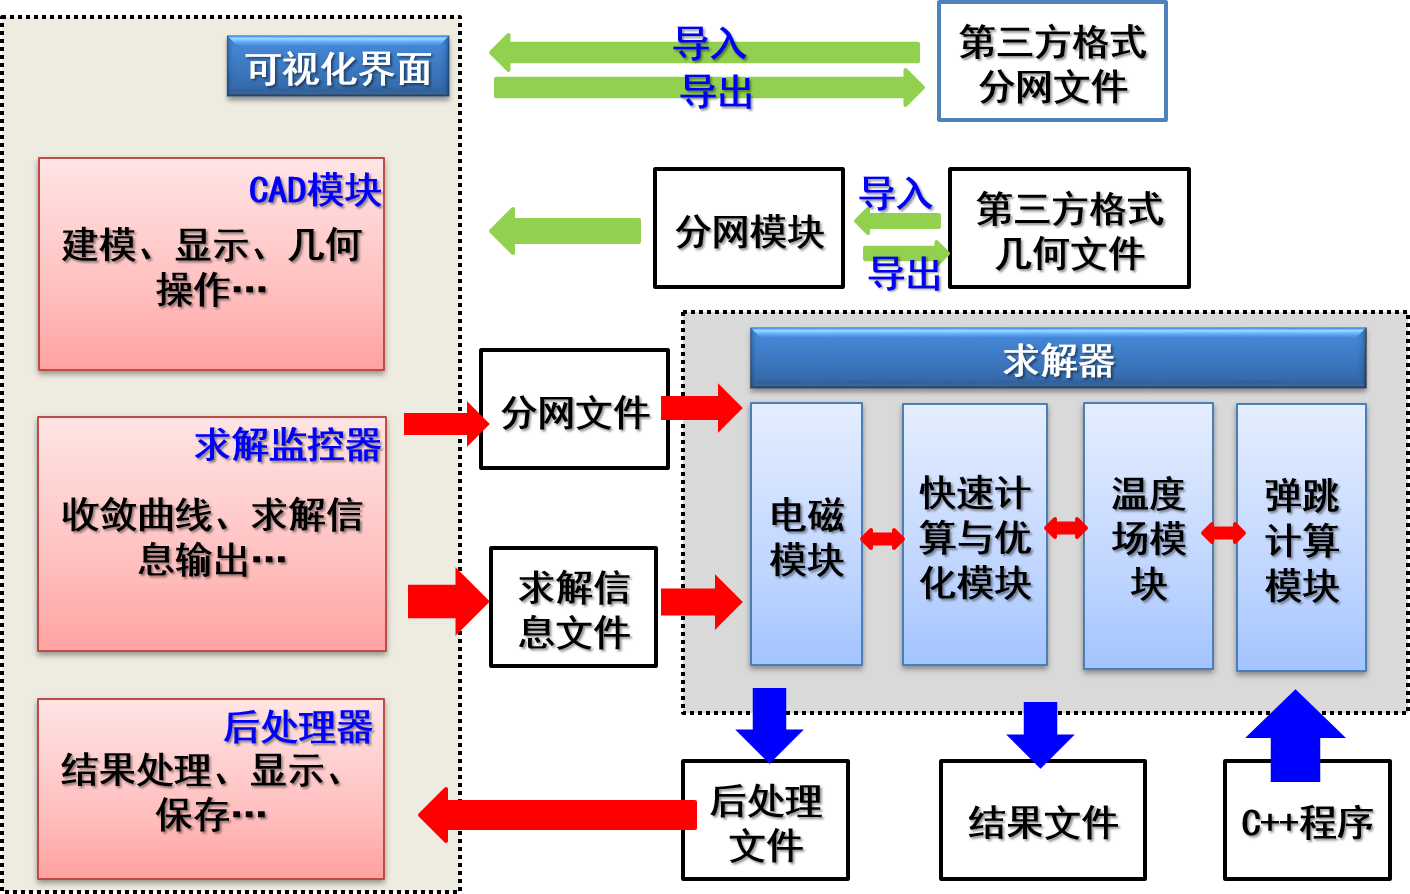
\includegraphics[width=0.7\linewidth]{figures/softarch}
	\caption{软件FEEM整体设计框架}
	\label{fig:softarch}
\end{figure}

\subsection{磁场问题的有限元求解}

\subsubsection{静磁场}

\subsubsection{瞬态磁场}
在电器当中的瞬态问题,主要还是考虑到可动部件的运动。

静态特性

在静态特性计算当中,可运动部件并没有真的在运动。只不过相对固定部分发生一定的位移之后,计算出电磁场的分布。求解的是一组静磁场问题。也没有考虑任何的动态方程,等同于针对位移的参数求解。

动态特性

实际的仿真过程需要考虑运动的耦合。电磁-运动的耦合是一种电磁问题和运动学问题的弱耦合。在每一个时间步的计算当中,先求解电磁场问题,然后再求解运动学问题,求解过程如下:

1.求解麦克斯韦方程组,计算发生一定位移后,施加在运动部件上的电磁力或电磁力矩;

2.求解运动部件的动态方程,计算出运动部件在时间步内的加速度值和速度,并且计算出下一时间步时运动部件新的位移位置;

3.将运动部件移动到新的位置,并且进行重分网操作;

4.返回步骤1。

\subsection{电磁力的计算}

Arkkio’s method


各种方法的优缺点对比

stress tensor方法的缺点

在数学上,这种方法是完全正确的,能够得到准确的力矩值,前提是B的计算值是准确的。然而,通常情况下不是这样的。需要注意的是,有限元求解是一种数值计算方法,因此,我们大多数情况下处理的都是近似值。特别地,我们实际求解得到的是磁势向量A,而磁感应强度B是通过计算A的旋度来得到的。这实际上是一个微分过程,如果我们对某些不准确的变量进行了微分操作,那么最后得到的计算结果必然也是有误差的。也就是说,我们计算得到的B的误差将会比A的误差更大。如果能够取消这个微分计算的过程,那么将有可能提高计算精度。
\subsection{优化问题}

\section{界面设计}

\subsection{Ribbon模块}
Ribbon模块是一个能够提供类似Office界面风格的组件。同时,COMSOL采用的也是类似界面。

1.如何自定义Ribbon的主题?
\subsection{QtFLEX模块}
该模块实现类似Visual studio当中的可停靠用户界面的组件。窗口内部的子部件可以根据用户随意的进行位置放置。可以设置自动隐藏停靠,可以与其他窗口进行分割,合并。
\begin{figure}
	\centering
	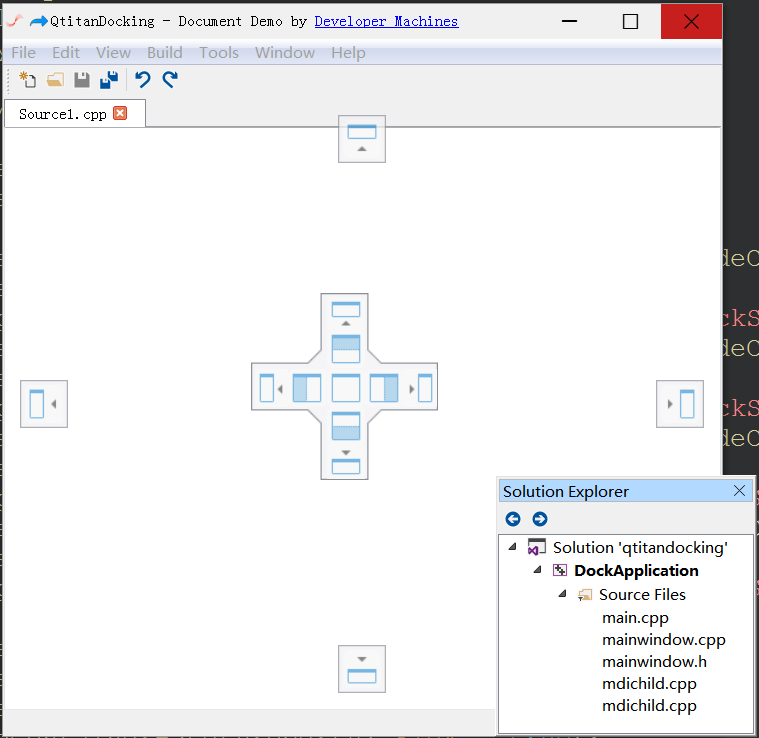
\includegraphics[width=0.7\linewidth]{figures/dock}
	\caption{Dock演示}
	\label{fig:dock}
\end{figure}

\subsection{界面布局}

\section{定义}
为了对数据进行存储,需要定义合理的格式和存储方式。
\subsection{工程文件格式及存储}
工程文件,即是软件会打开的文件,通过读取这个文件,软件可以获得该项目当中的几何模型、物理设置参数、分网信息、求解信息等。目前,最普遍的方式就是采用标记式语言进行存储,首选XML语言。
\subsection{几何文件格式及存储}
几何图形是用户在操作软件过程当中一直会使用到的东西,所以这部分数据肯定是常驻内存。在软件的核心,需要定义几何存储的格式来代表各种图形,这些图形可以是用户自己创建的,也可以是不同格式的几何文件转换过来的。
\subsection{分网文件格式及存储}
跟几何文件类似,也需要在工程内部自定义分网数据格式,来保存从各种格式的分网文件读取并转换而来的数据。
\subsection{结果数据文件及存储}
在求解结束后,需要一个数据结构来存储计算得到的各种数据结果。
\subsection{编程代码规范}
为了使软件开发尽量的规范,开发小组成员应当遵守以下操作:
\section{CAD绘图}
几何绘图是软件可视化最重要的一个部分。
\subsection{绘图原理}
在显示屏上你所看到的有趣的东西,都是程序员尽力地让一切看起来都跟真的似的,实际上,它依旧还是冷冰冰的机器,只是用的时间长了可能会发热而已。

\begin{enumerate}
	\item 图形的显示
	
\hspace*{2em} 图形在显示器上的显示效果,是我们通过程序进行渲染的结果。
	\item 图形的选中
	
\hspace*{2em} 图形的选中效果也是一种修饰,让用户感觉鼠标所单击的实体被选择了。实现方式就是绘制一个选中的效果,虚线框或者其他示意形状。那么如何方便的添加这个功能效果呢?简单的思路就是在每一个实体当作添加一个选中判断的函数,如果选中了,那么就返回一个相应的实体添加到选中实体的列表当中,然后调用重绘命令就可以了。
\end{enumerate}
\subsection{基本几何形状}
需要实现的基本几何形状有:点、线、圆弧、(长)方形、多边形、(椭)圆等。
\subsection{坐标网络的绘制}
绘制几何图形之前,需要建立一个绘制的画布,也就是具有横纵坐标的网格区域。需要注意的是,坐标轴上显示的数值跟屏幕上像素点的位置不是一样的,需要进行一下转化。

大多数的有限元仿真软件似乎不提供数学上的那种坐标轴网络,只有COMSOL是这样做的。我觉得提供一个坐标轴的显示还是比一个空白的背景要好很多。其实,flux2d也是有的,在你刚新建一个项目的时候会出现。
\begin{figure}
	\centering
	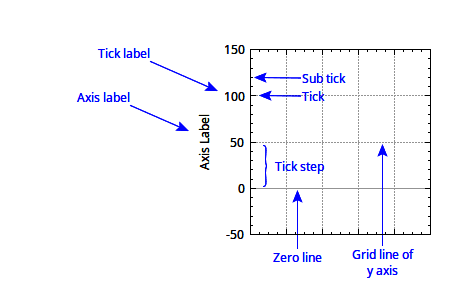
\includegraphics[width=0.7\linewidth]{figures/AxisNamesOverview}
	\caption{}
	\label{fig:axisnamesoverview}
\end{figure}
\begin{figure}
	\centering
	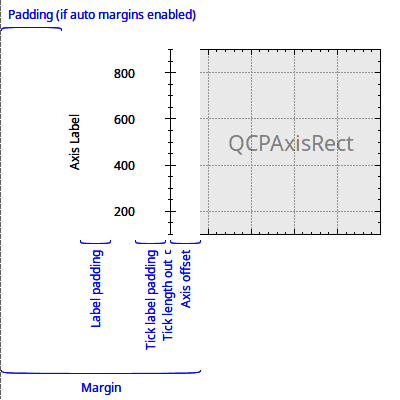
\includegraphics[width=0.7\linewidth]{figures/AxisRectSpacingOverview}
	\caption{}
	\label{fig:axisrectspacingoverview}
\end{figure}

接下来记录一下如何开发一个比较不错的简单坐标轴系统。

\begin{enumerate}
	\item 首先,需要建立一块画布,QWidget或者其子类,需要在上面进行绘图。这个画布类当中包含有各种画图需用的数据。
	\item 为了显示实际绘制的图形坐标而不是像素,需要一个基本的坐标轴,初始化的时候有一个默认的坐标轴大小区域。由于坐标轴的刻度与像素是一一对应的,所以,在绘制每一个图形之前,都需要调用坐标轴的转换函数来转换坐标,然后再绘制在画布上。需要注意的是,绘制的区域是有限制的,是被坐标轴所限制的,不能绘制在坐标轴之外。对于图形的缩放,似乎不需要特别处理,只需要更新一下坐标轴的范围,然后进行重画就可以了。
	\item 那么重头戏就是坐标轴了。
\end{enumerate}

主要功能:
\begin{enumerate}
	\item 状态栏显示鼠标指针所指的坐标轴内的坐标;
	\item 缩放功能;
	
\hspace*{2em} 可以在各种软件当作体验一下。以缩小为例,不断滚动鼠标滚轮,坐标轴网格会以鼠标指针所在的位置为中心缩小,缩小到一定程度子刻度网格不再显示,然后重新开始下一轮网格的缩放。坐标轴上的可以也会随缩放不断改变。
	\item 坐标轴外部不能绘图;

\hspace*{2em} 可以考虑clipRect函数。
\end{enumerate}

为了绘制一个长方形的坐标轴区域,在编程之前可以进行模块分解以及数据抽象。该长方形区域包含四个轴,因此可以抽象出“轴”这个类;然后对轴进行分解,可以包含轴线、刻度、刻度标签文本、网格等等,可以分别建立相应的类。
\subsection{形状操作}
所谓的用户能够对显示的几何形状进行控制,实际上是程序针对用户的鼠标操作与实际几何形状的位置进行了比较计算之后,进行了一些算法。每一次改变都会导致显示内容的刷新,只不过肉眼无法辨别出来。
\subsubsection{形状选中、调整大小、删除、隐藏显示}
每一个形状需要接受鼠标事件,单击可以被选中,绘制出被选中的效果,或者绘制外边框,或者改变形状的填充效果。

形状被选中后,可以进一步的调整形状的尺寸大小。外边框上会显示调控点。可以进一步地进行拖拽操作。

形状选中后,可以被移动到新的位置。
\subsubsection{自动吸附}
点坐标的自动捕捉,用来帮助我们快速地选择已有的一些点的坐标,方便进行图形的快速绘制。实现原理就是根据当前的鼠标坐标点,从几何实体列表当中去寻找,哪一个实体的哪一个点离该点最近,在捕捉精度范围内,那么该点就可以被捕捉到。如果是自由模式,就只捕捉当前的鼠标指针位置即可。
\subsubsection{布尔操作}

\subsubsection{缩放、变形}

\subsection{与分网显示、后处理的接口}

\subsection{参数绘图}

\section{材料库}
为了对模型当中的结构添加相应的材料属性,需要提供一个材料管理器的功能,能够存储一些常见的材料,并且能够实现新建、修改、删除等操作。
\subsection{已有材料库}

\subsection{新建、删除材料}

\subsection{导入、导出材料}

\section{分网生成}
分网无疑是有限元器求解最为关键的步骤之一。
\subsection{分网读取、导出}

\subsection{有限元分网形状}

\subsection{读取几何模型并分网}

\subsection{分网控制}

\subsection{删除分网}

\subsection{分网可视化}

\section{求解器}

\subsection{求解器设置}

\subsection{优化模块}
当所有的求解信息都设置好后,不仅可以实现磁场的求解,还能够实现对某些参数的优化设计。

\subsection{收敛曲线显示}

\section{后处理}
求解器计算得到的结果无疑要使用最好的方式展现给用户。
\subsection{结果曲线}

\subsection{结果云图}

\subsection{结果矢量图}

\subsection{数据导出}
\chapter{测试模型}
\chapter{自动化}
这一部分是规划中的未完成项目。
\section{使用CMake编译Qt程序}
Qt官方的关于CMake的使用:\href{https://doc.qt.io/qt-5/cmake-manual.html}{CMake手册}
\chapter{求解器}
有限元软件通常以求解单场或者多场为目的,因此,需要在求解之前建立对应的单场或者多场的求解数据模型,以便完成目标物理现象的求解任务。这些求解模型一般会是静态的或者变化的,通常会包含常见的非线性问题。一般的求解步骤是,将所要求解的偏微分方程组转化为弱形式,然后进行有限元近似,得到待求解的方程组,最后,采用不同的方法进行求解,得到计算结果。
\section{求解所需要素}
\begin{enumerate}
    \item 分网文件
\end{enumerate}
\section{单场的求解过程}

\section{多场的求解过程}

\section{线性系统的求解}



\chapter{求解模型}
每一种物理场都有对应的偏微分方程(组),为了得到模型的结果,需要对方程进行离散求解。
\section{三维电磁场}
               
\section{二维电磁场}

\section{有限元模型}
设计有限元的类,需要保存什么?还需要考虑的是怎样保存的问题?进一步地就需要实现怎样去获取这些东西?用户应该如何输入操作来生成这样的数据。
\begin{enumerate}
	\item 求解模型的纬度,坐标系
	\item 单元数,节点数,边界条件数
	\item 单元列表
	\item 节点列表
	\item 初始条件
	\item 边界条件
	\item 材料列表
	\item 求解域内的方程
	\item 求解区域的列表,每一个求解区域应当包含材料,初始条件,边界条件和方程等
	\item 求解器接口
\end{enumerate}
\section{求解过程}
主要描述一下基本的有限元求解过程,主要指的是数值实现方面。
\chapter{研究}
研究一些基本的数据,建立基本的概念,合理地设置数据模型。倾向于如何更好地设计一个软件方面的思想。市场上有那么多的技术,到底哪个好啊,用哪个比较不错啊。A这样写感觉非常的简洁,B那样写好像更好一点,采用哪个就成了难题。
\url{https://blog.csdn.net/sinat_20265495/article/details/52004082}
\url{https://blog.csdn.net/hzm8341/article/details/70941698}
\url{https://blog.csdn.net/jonathan321/article/details/78106101}

\section{如何高效、优雅的地设计C++的类?}
\subsection{类的需求}
1、设计该类的目的

清晰的概念远比模棱两口的理解,更能帮助我们深入分析问题。有时候我们觉得我就是需要实现这个功能罢了,只要能用就好了。然而,多和产品经理或技术经理沟通,有可能出现意想不到的结果:

该功能没有我们想到那么复杂,并不需要自己设计;

该功能比我们想到的更加复杂,我们需要考虑更多正确性、高效性、扩展性、维护性等方面的额问题。

2、使用该类的场景

不同的使用场景,相同功能类的设计需求是不一样的。譬如,设计一个视频解码类,如果使用场景为视频播放器,那我们设计的类必须要考虑不同的编码格式;但如果使用场景为视频会议,我们设计的类就不需要考虑太多编码格式的问题,反而需要针对某种格式进行效率优化。

3、潜在的扩展方向

程序不是一成不变的,外界事物不停的变化,催生不同的需求。如果我们的程序不可扩展,那每次需求变更,之前的工作都白费了。类的设计一定要考虑到,未来潜在的扩展方向。如果我们无法确定潜在的扩展方向,至少留下可扩展的接口,不要把一切行为、属性都写死。
\subsection{构造函数、析构函数、拷贝赋值}
C++类的构造析构和拷贝赋值是设计C++类时最基本的要点,有不少细节部分需要考虑:

构造函数:合成的默认构造函数、默认构造函数、default关键词、explicit关键字、类型转换、延迟初始化、单例模式

析构函数:默认析构函数、虚析构函数

拷贝构造函数:深拷贝/浅拷贝、禁止拷贝

赋值构造函数:深拷贝/浅拷贝、禁止拷贝

除了上面的细节部分,我们需要明确几个准则:

除非默认操作非你所需,否则请用=default来定义构造析构函数;

除非编译器合成为你所需,否则请用=delete来定义赋值拷贝函数;

除非类不可能成为基类,否则请将析构函数定义为virtual;

构造与析构过程中,不调用virtual函数、析构函数不能抛出异常。

拷贝构造复制需要处理深拷贝和浅拷贝,赋值操作需要额外考虑自我赋值。【浅拷贝】只是增加了一个指针,指向已存在对象的内存。【深拷贝】是增加了一个指针,并新开辟了一块空间,让指针指向这块新开辟的空间。【浅拷贝】在多个对象指向一块空间的时候,释放一个空间会导致其他对象所使用的空间也被释放了,再次释放便会出现错误。

\subsection{如何设计接口?}
\section{如何实现一款有限元软件?}

\section{工程结构}
一个良好的工程目录结构,不仅能够帮助你整理思路,而且能够让源代码的阅读者更加容易的理解你的工程内容。看了太多的源代码,发现不同的团队,开发的风格真的是迥异。

\subsubsection{Qbs}
Qbs是一种构建自动化工具,旨在方便地管理跨多个平台的软件项目的构建过程。


\subsection{如何进行插件式的开发?}
其实,也没有完全必要进行这种开发,只是觉得这种写法真的是非常的优雅,有用。逻辑清晰,模块之间相对独立,便于调试。

主要的思路就是每一个模块都是生成独立的链接库或者可执行程序。但是,这样的东西其实看这个模块跟主模块有没有耦合关系。我觉得有关系的才能叫做插件吧?比如,模块需要访问主程序当中的某一个接口,要创建自己的菜单或者界面,真正的成为一个主界面的一部分。如果就只是独立的程序话,就相当于单纯的函数调用而已。不,插件的意思应该是主程序在编写的时候不知道有什么具体功能的插件。所以说,并不是所有的链接库都能称之为插件。qtcreator的方式应该是那种自动的在插件目录寻找符合插件要求的,然后作为插件载入。而Salome应该是手动载入的调用的,每一个功能作为单独的模块来写,然后在主程序当中进行调用。研究了一下,发现qtcreator的源代码里,两者都是包含的,一个是称作library,一个是称作plugin。其中,library是放在exe的路径下的,而plugin是放在特定的目录下去动态载入的。

那是不是可以把这个问题归结为主程序应当如何读取插件信息?哪些东西要作为插件?哪些没有必要?我认为,那些被动调用的类库需要作为单纯的库来写,而那些需要访问主插件信息的,可以考虑作为插件来写,前提是,自己具有一个插件的扩展系统。如果软件只是内部开发的话,不大的规模可以不考虑这种情况,毕竟对扩展性没有那么大的要求。

如果要开发动态链接库,需要注意:1.链接库需要放在exe程序能够找到的路径,一般跟exe在相同的路径,或者将路径加入到PATH当中;2.链接库项目有固定的写法,需要在头文件当中定义一个export的宏,然后如果是链接库项目,需要在pro文件添加DEFINE定义,使得类库是导出的,而在调用的时候,由于没有这个定义,类就是要导入的了。如果不写成链接库这种形式的话,那么你的所有的代码都要编译进你最终的exe程序,非常的不合理。

那么链接库怎么使用呢?使用的时候,需要头文件和链接库的路径。需要的头文件应该还是要单独的写到app的pro文件当中去的,不知道会不会自动添加。
\section{链接库的原理及使用}
\subsection{动态链接库}
Linux 采用 ELF 格式,源头我不大清楚,似乎是个相当标准化的格式,很多操作系统都用。似乎 ELF 没有按索引号导出的功能,装载器负责给可执行程序填好引入表。很规范,没什么好说的。

DLL 是PE格式,它允许导出表中没有名字表。这个就是区别所在了。没有名字就无法根据名字链接,这种情况下需要 .lib 来协助。不用名字表链接时麻烦一些,但是运行时还是有好处的,载入速度会快一些,也省一点内存。另外,windows下静态库也是 .lib 。微软给这两个不同用途的文件都用 .lib 后缀真是心大。

用 dumpbin 看 dll,用 nm 看 so,其实它们的信息基本上差不多的,但是有的DLL导出项没有名字或者有名字的项特别少,so 就不会这样,它的导出项都有名字的。看可执行程序也一样:Windows 的可执行程序引入表是可以简略名字直接用序号的,对有些 DLL 的导入项根本没有名称(根据优化参数而异),只有序号。而Linux 的可执行程序的引入表总是有完整的名称。

总的说,在 DLL 没有做名字表优化的情况下(大多如此),.lib 其实并不是必须的,也有工具可以从 DLL 直接生成一个 .lib。但是……我也不知道没有 .lib 情况下如何 implicit link。
\subsection{静态链接库}
\subsection{如何识别lib文件为静态链接库还是导入库?}
\section{Python脚本与C++程序的结合}

\section{Qt}
\subsection{Q\_DECLARE\_METATYPE}
这个宏是为了让QMetaType知道Type这个数据类型,并提供一个默认的拷贝构造函数和析构函数。QVariant需要使用Q\_DECLARE\_METATYPE这个宏来定制类型。

当使用这个宏的时候要求Type是一个完整的数据类型。可以使用Q\_DECLARE\_OPAQUE\_POINTER()来注册一个指针用于转发声明类型。

一般都把这个宏放到结构体或类的末尾【注意:这是官方说的】,如果不放到末尾也是阔以的,就放到头文件中,当你用 QVariant就要包含那个.h,个人觉得这非常不适合面向对象以及模块化编程。

通过添加Q\_DECLARE\_METATYPE()这个宏让QOject及其子类知道这个类型。这里要注意的是如果要在队列信号(关于connect函数队列信号请看这篇博文:https://blog.csdn.net/qq78442761/article/details/81937837)中使用或者用用槽连接,要先调用这个函数qRegisterMetaType()【这里是在运行的时候,对他进行注册】

\subsubsection{Qt 常用命令,宏,pro文件格式}
\begin{lstlisting}
qmake 常用命令:
qmake -project //生成pro文件,自动检查c/c++程序文件
qmake -t lib     //生产把源码编译成库的pro工程文件
qmake -tp vc //根据pro文件生成vc的工程文件,qt commericial有一个绑定到vs的具,可以在菜单栏直接打开
qmake -r xxx.pro "CONFIG+=debug" //递归生成makefile
moc //包含Q_OBJECT文件转换器
rcc //Qt resource compiler
uic //Qt ui file translator,to .h file.
Qt 常用宏:
平台相关
Q_WS_WIN //window系统
Q_WS_X11 //xwindow系统
Q_WS_MAC //苹果mac系统
Q_WS_SOL //sun的solaris系统
其它
QT_OPENGL_SUPPORT //是否支援opengl
QT_VERSION    //qt的版本,如 if QT_VERSION > 0x040601(qt > 4.6.1)
QT_VERSION_STR //qt版本的字符串
QT_POINTER_SIZE //指针的字节宽度 32bit=4,64bit=8
QT_REQUIRE_VERSION //用在代码中,比如QT_REQUIRE_VERSION(argc, argv,"4.0.2");
global常用函数
T qAbs(const T & value) //返回绝对值
void	qCritical(const char * msg, ...) //
void qDebug(const char * msg, ... ) //
void	qFatal(const char * msg, ... ) //输出错误信息
qMax(const T & value1,const T & value2 )//
qMin(const T & value1,const T & value2 ) //
  
pro 文件格式
#: 表示到行尾均为注视,被忽略
include: 可以包含别的文本文件,一般为*pri 例如 #include "../global.pri"
scope{;;}: 预定义 ,如win32{} 表示在win32平台下的定义,其它忽略
win32/unix/linux-g++/linux-g++-64: 平台宏
DESTDIR: 产生目标文件路径
MOC_DIR: moc转换文件路径
RCC_DIR: 资源文件路径
UI_DIR:ui文件转换的路径
LIBEXT: 产生lib的后缀
QMAKE_CFLAGS_DEBUG:
QMAKE_CXXFLAGS_DEBUG:
QMAKE_CFLAGS_RELEASE:
QMAKE_CXXFLAGS_RELEASE:
TEMPLATE: 决定生成makefile采用的模板,
 =lib 表示库文件
 =app 表示生成可执行文件
 =subdirs 表示处理子目录(在下面用SUBDIRS += **来指定那些子目录)
TARGET: 指定目标文件名
Qt+=: 添加额外的模块支持,例如Qt -= QtCore;Qt += network,phonon,xml,thread
DEFINES: 添加额外的宏定义,如win下需要的export等
DEPENDPATH: 添加以来的路径
INCLUDEPATH: 添加头文件包含路径
HEADERS: 需要包含的头文件
SOURCES: 需要包含的源文件
FORMS: 需要包含的ui文件
RESOURCES:需要包含的资源文件
LIBS:依赖库的路径和名称 -L{xxdirxx} -l{xxnamexx}
CONFIG: 添加配置,如warn_on debug_and_release plugin
TRANSLATIONS: 多国语言支持文件
INSTALLS: 要安装的文件
target.path: 安装的路径
#在pro文件支持environment variables和自定义变量
#如sources.file += $$SOURCES $$HEADERS
#sources.path = $$DESTIN_DIR
#INSTALLS += target source
defineReplace(xxx): xxx为变量 ,此函数可以返回一个变量值如:$$xxx()
exists(file1,file2){error()}:检查文件是否存在   
\end{lstlisting}
\section{C++}
\subsection{左值、左值引用、右值、右值引用}
\subsubsection{左值和右值的概念}

左值是可以放在赋值号左边可以被赋值的值;

左值必须要在内存中有实体;

右值当在赋值号右边取出值赋给其他变量的值;

右值可以在内存也可以在CPU寄存器。

一个对象被用作右值时,使用的是它的内容(值),被当作左值时,使用的是它的地址。

\subsubsection{引用}

引用是C++语法做的优化,引用的本质还是靠指针来实现的。引用相当于变量的别名。

引用可以改变指针的指向,还可以改变指针所指向的值。

引用的基本规则:

声明引用的时候必须初始化,且一旦绑定,不可把引用绑定到其他对象;即引用必须初始化,不能对引用重定义;
对引用的一切操作,就相当于对原对象的操作。

\subsubsection{左值引用和右值引用}

1 左值引用

左值引用的基本语法:type \&引用名 = 左值表达式;

2 右值引用

右值引用的基本语法type \&\&引用名 = 右值表达式;

右值引用在企业开发人员在代码优化方面会经常用到。

右值引用的“\&\&”中间不可以有空格。

\subsection{虚函数}

虚函数放在一张表里(非标准,只是编译器实现虚函数的一般手段)。表中放类型信息和虚函数地址。带虚函数的类与普通的类不同之处在于多了一个虚表指针,并且由于可以通过虚表指针找到自己的动态类型,所以可以进行dynamic\_cast。

扩展:构造函数是否为虚函数(不知道为什么都喜欢问这种无聊的问题)、析构函数什么时候需要是虚函数、虚继承的类内布局(MSVC有单独的指向虚基类表的指针)、虚基类中有虚函数的类内布局(这样子类如果要有新的虚函数的话,有可能会有两个虚函数表)、多重继承的类内布局(多个虚函数表,指向第二个及以后的基类指针会有隐式指针的转换,析构会转换回来)、Itanium C++ ABI(两个delete函数)、MSVC C++ ABI、使用cl filename /d1 reportSingleClassLayoutClassName查看类内布局。

\subsection{多态}

模板(参数多态)、模板特化和函数重载(特设多态)、模板偏特化和sfinae和concept(限定多态)、继承(子类型多态)、CRTP(静态多态)、动态类型绑定(动态多态)。

\subsection{堆内存}

堆内存由malloc分配,小于128k由brk分配连续的堆内存(第一次会分配33页出来),大于128k由mmap分配离散(按页对齐)的堆内存。malloc(size\_t n)分配的内存会比n大一些,多出来的是一些记录管理需要使用的内存。

扩展:operator new的22种重载格式、placement new(可不可以用作栈空间,std::variant的实现)、std::vector使用1.5倍扩容比使用2倍扩容会有什么优势、mmap为什么离brk指针那么远、glibc管理堆内存的方式。

\subsection{inline和static的语义}
inline的意思是linker去检查函数或变量的时候只保留一份副本,而不会报重定义的错误。和函数体是否inline展开没有任何关系。

static的意思分为两种。非类内的static是指当前的变量放在数据段而不是栈段,并且拉黑linker,使得linker看不到它。类内的static则是没有this指针的隐含参数,是类拥有这个static变量或函数,而不是对象。

\subsection{lambda}
lambda就是函数对象的语法糖。没有捕获的lambda可以转化成函数指针(使用取正+操作符隐式转换)、引用捕获和值捕获、lambda可以被内联优化、lambda使用auto参数列表实现泛型。

扩展:C++20中对lambda的改进、使用lambda(或者函数指针)可以把数据包起来放在模板参数中、继承lambda实现std::visit。

\subsection{智能指针}
std::shared\_ptr的control block(为什么有weak count,delete的类型擦除,引用计数的线程安全)、std::make\_shared的control block和对象连在一起、std::enable\_shared\_from\_this实现原理(CRTP)、std::unique\_ptr对T[]类型的偏特化,std::unique\_ptr的实现(RAII)。

扩展:如何设计std::make\_shared的内存对齐、如何设计std::shared\_ptr使得其支持T[]、std::experimental::observer\_ptr和裸指针的区别。

\subsection{模板实参推导}
三种模板参数如何推导的(T,T\&,T\&\&)、auto如何推导的(auto,auto\&,auto\&\&)、decltype(auto)如何推导的、引用折叠(为什么const T\& with [T = int\&]会折叠成int\&而不是const int\&)、为什么类模板的参数包必须放在模板参数的最后而函数模板不用。
\section{Qt 中的二进制兼容策略}

本文翻译自
\href{https://link.jianshu.com?t=https://community.kde.org/Policies/Binary\_Compatibility\_Issues\_With\_C\%2B\%2B}{Policies/Binary
Compatibility Issues With C++}

\subsection{二进制兼容的定义}\label{ux4e8cux8fdbux5236ux517cux5bb9ux7684ux5b9aux4e49}

如果程序从一个以前版本的库动态链接到新版本的库之后,能够继续正常运行,而不需要重新编译,那么我们就说这个库是二进制兼容的。

如果一个程序需要重新编译来运行一个新版本的库,但是不需要对程序的源代码进一步的修改,这个库就是源代码兼容的。

二进制兼容性可以节省很多麻烦。这使得为特定平台分发软件变得更加容易。如果不确保版本之间的二进制兼容性,人们将被迫提供静态链接的二进制文件。静态二进制文件不好,因为它们

\begin{itemize}

\item
  浪费资源(尤其是内存)
\item
  不能让程序从库中错误修正或扩展中受益
\end{itemize}

\subsection{如何确保二进制兼容}\label{ux5982ux4f55ux786eux4fddux4e8cux8fdbux5236ux517cux5bb9}

\subparagraph{在确保二进制兼容的情况下,我们能做的操作:}\label{ux5728ux786eux4fddux4e8cux8fdbux5236ux517cux5bb9ux7684ux60c5ux51b5ux4e0bux6211ux4eecux80fdux505aux7684ux64cdux4f5c}

\begin{itemize}

\item
  增加非虚函数、signal/slots、构造函数
\item
  增加枚举到类中
\item
  在已经存在的枚举的最后添加枚举值

  \begin{itemize}
  
  \item
    例外:如果这会导致编译器为枚举选择更大的底层类型,那么更改会导致二进制不兼容。需要注意的是,编译器有选择基础类型的余地,所以从
    API 设计的角度来看,建议添加一个 Max
    枚举,其中包含一个明确的最大值(=255 或 =1 \textless{}\textless{} 15
    等)来创建一个数字枚举数值的区间,使其无论如何能够保证适合所选择的底层类型。
  \end{itemize}
\item
  重新实现在父非虚基类
  (从当前类回溯第一个非虚基类)里定义的虚函数,但是这个不完全确保二进制兼容,所以尽量不要这么做

  \begin{itemize}
  
  \item
    例外: C++
    有时候允许重写的虚函数改变返回类型,在这种情况下无法保证二进制兼容。
  \end{itemize}
\item
  修改内联函数,或者把内联函数改成非内联的。这个不完全确保二进制兼容,所以尽量不要这么做
\item
  去掉类里一个 private 的非虚函数,并且这个函数没有被任何 inline
  函数调用过
\item
  去掉类里一个 private 的静态变量,并且这个变量没有被任何 inline
  函数调用过
\item
  增加一个静态成员变量
\item
  增加新类
\item
  导出以前未导出的类
\item
  增加或者减少类的友元声明
\item
  重命名原有成员变量
\item
  原有的成员位宽扩大或缩小,但扩展后不得越过边界(char 和 bool 不能过 8
  位,short 不能过 16 位,int 不过 32 位,等等)
\item
  为原本继承自 QObject 的类添加 Q\_OBJECT 宏
\item
  添加 Q\_PROPERTY、Q\_ENUMS 或 Q\_FLAGS 宏,因为它们只是修改由 moc
  生成的元对象而不是类本身
\end{itemize}

\subparagraph{在确保二进制兼容的情况下,严格禁止的操作:}\label{ux5728ux786eux4fddux4e8cux8fdbux5236ux517cux5bb9ux7684ux60c5ux51b5ux4e0bux4e25ux683cux7981ux6b62ux7684ux64cdux4f5c}

\begin{itemize}
\item
  对已经存在的类进行:

  \begin{itemize}
 
  \item
    把原本已经导出的类,进行取消或删除导出操作
  \item
    以任何方式更改类层次结构(添加,删除或重新排序基类)的操作
  \end{itemize}
\item
  对于类模板进行:

  \begin{itemize}
  
  \item
    以任何方式更改模板参数(添加,删除或重新排序)的操作
  \end{itemize}
\item
  对于已经存在的函数进行:

  \begin{itemize}
  
  \item
    取消对外开放(共有改为私有)的操作
  \item
    删除函数的操作

    \begin{itemize}
    
    \item
      删除现有声明函数的实现的操作
    \end{itemize}
  \item
    改成内联的(把代码从类外实现移到头文件的类内实现也算是内联的)操作
  \item
    增加重载操作,向已经重载的函数添加重载是可以的
  \item
    改变函数特征,这包括:

    \begin{itemize}
    
    \item
      修改参数列表中任何参数的类型,包括改变现有参数的 const 或者
      volatile
      限定符。如果必需要这么做,可以通过增加一个新函数的方法来实现
    \item
      改变函数的 const 或者 volatile 限定符
    \item
      把 private 改成 protected 或者
      public。如果必需要这么做,可以通过增加一个新函数的方法来实现
    \item
      更改成员函数的 CV 限定符:应用于函数本身的 const 和/或 volatile
    \item
      用另一个参数扩展一个函数,即使这个参数有一个默认值
    \item
      以任何方式改变返回类型
    \item
      例外:用 extern``C''
      声明的非成员函数可以改变参数类型,但是尽量不要这么做
    \end{itemize}
  \end{itemize}
\item
  对于虚成员函数进行:

  \begin{itemize}
  
  \item
    将虚函数添加到没有任何虚函数或虚基类的类
  \item
    将虚函数添加到被别的类继承的类
  \item
    在 Windows
    上,出于任何原因添加新的虚函数,即使是在无任何子类的类中。这样做可能会重新排序现有的虚拟功能并破坏二进制兼容性
  \item
    改变类声明中虚函数的顺序
  \item
    如果一个函数不是在父非虚基类
    (从当前类回溯第一个非虚基类)中声明的,覆盖它会造成二进制不兼容
  \item
    如果虚函数被覆盖时改变了返回类型,不要修改它
  \item
    删除一个虚函数,即使它是从基类重新实现一个虚函数
  \end{itemize}
\item
  对于静态非私有成员或非静态非成员公共数据进行:

  \begin{itemize}
  
  \item
    改成不对外开放的或者删除
  \item
    改变其类型
  \item
    改变其 const 和/或 volatile 限定符
  \end{itemize}
\item
  对于非静态成员:

  \begin{itemize}
  
  \item
    将新的数据成员添加到现有的类
  \item
    改变一个类中的非静态数据成员的顺序
  \item
    修改成员的类型,修改符号例外 (例如:signed/unsigned
    改来改去,不影响字节长度)
  \item
    从现有的类中删除现有的非静态数据成员
  \end{itemize}
\end{itemize}

如果需要添加扩展/修改现有函数的参数列表,则需要添加新的函数,而不是新的参数。
在这种情况下,我们可能需要添加一个简短的提示,即在更高版本的库中,这两个函数应与默认参数合并:

\begin{lstlisting}
void functionname( int a );
void functionname( int a, int b ); //BCI: merge with int b = 0
\end{lstlisting}

为了使我们的类在未来能够有序的扩展,我们应该遵循这些规则:

\begin{itemize}

\item
  为类添加 d 指针
\item
  添加非内联虚析构函数,即使在析构函数的实现中我们什么也不做,那就让它为空好了
\item
  QObject
  派生类中的重新实现事件,即使函数的主体只是调用基类的实现,也要将其实现
\item
  使所有构造函数非内联
\item
  编写拷贝构造函数和赋值运算符的非内联实现,除非该类不能被值拷贝(例如,从
  QObject 继承的类不能)
\end{itemize}

\subsection{类库开发技巧}\label{ux7c7bux5e93ux5f00ux53d1ux6280ux5de7}

编写类库时最大的问题是,不能安全地添加数据成员,因为这可能会改变包含该类型对象(包括子类)的每个类、结构或数组的大小和布局。

\subparagraph{位标志}\label{ux4f4dux6807ux5fd7}

一个解决办法就是利用位标志。比如你原来设计了一个类,里面有如下的几个
enum 或者 bool 类型:

\begin{lstlisting}
uint m1 : 1;
uint m2 : 3;
uint m3 : 1;
\end{lstlisting}

如下的修改不会破坏二进制兼容:

\begin{lstlisting}
uint m1 : 1;
uint m2 : 3;
uint m3 : 1;
uint m4 : 2; // new member
\end{lstlisting}

究其原因,是本来已经占用了足够的位数,增加一个位标志并没有让数据字节长度增加。注意:请舍入到最多
7 位(如果位域已经大于 8,则为
15)。使用最后一位可能会导致一些编译器出现问题

\subparagraph{使用 d 指针}\label{ux4f7fux7528-d-ux6307ux9488}

位标志和预定义的保留变量很好,但远远不够。这是 d
指针技术发挥作用的地方。``d-pointer'' 这个名字源于 Trolltech 公司的 Arnt
Gulbrandsen,他首先将这项技术引入到 Qt
中,使其成为第一个在大版本之间保持二进制兼容性的 C ++ GUI 库之一。
所有看过它的人都很快将这种技术作为 KDE
库的一般编程模式。这是能够在不破坏二进制兼容性的情况下将新的私有数据成员添加到类中是一个很好的技巧。

备注:在计算机科学的历史中,d
指针模式已经被通过多种名称被实现了很多次,例如, 作为 pimpl,作为
handle/body 或者 cheshire cat。 Google
可以帮助我们找到任何这些内容的介绍,只需将 C++
一起添加到搜索作为关键词即可。

在类 Foo 的类定义中,定义一个前向声明

\begin{lstlisting}
class FooPrivate;
\end{lstlisting}

和私有成员中的 d 指针:

\begin{lstlisting}
private:
    FooPrivate* d;
\end{lstlisting}

FooPrivate 类本身完全是在类实现文件(通常是* .cpp)中定义的,例如:

\begin{lstlisting}
class FooPrivate {
public:
    FooPrivate()
        : m1(0), m2(0)
    {}
    int m1;
    int m2;
    QString s;
};
\end{lstlisting}

现在我们要做的事情就是在我们的构造函数或 init 函数中创建私有数据

\begin{lstlisting}
d = new FooPrivate;
\end{lstlisting}

并在我们的析构函数中删除它

\begin{lstlisting}
if (d) {
    delete d;
    d = 0;
}
\end{lstlisting}

在大多数情况下,我们会希望使 d
指针避免不慎被修改或复制的情况,以免丢失私有对象的所有权并造成内存泄漏:

\begin{lstlisting}
private:
    FooPrivate* const d;
\end{lstlisting}

这允许我们修改 d 指向的对象,但是在初始化之后不能修改指针的值。

不过,我们可能不希望所有成员变量都存在于私有数据对象中。对于经常使用的成员,将它们直接放在类中会更快,因为内联函数不能访问
d 指针数据。还要注意,在 d 指针本身中声明了 d
指针所涵盖的所有数据都是``私有的''。
对于公共或受保护的访问,可以提供一个 set 和一个 get 函数。 例如:

\begin{lstlisting}
QString Foo::string() const
{
    return d->s;
}

void Foo::setString( const QString& s )
{
    if (d->s != s;) {
        d->s = s;
    }
}
\end{lstlisting}

也可以将 d
指针的私有类声明为嵌套的私有类。如果使用这种技术,请记住嵌套的私有类将继承包含导出的类的公共符号可见性。
这将导致私有类的功能在动态库的符号表中被命名。 我们可以使用
Q\_DECL\_HIDDEN 执行嵌套的私有类来手动重新隐藏符号。这在技术上是一个 ABI
的变化,但是不会影响到 KDE 开发者所支持的公众
ABI,所以被误认为是私密的符号可能会被重新隐藏而不会被警告。

\subsection{常见问题处理方法}\label{ux5e38ux89c1ux95eeux9898ux5904ux7406ux65b9ux6cd5}

\subparagraph{如何将新的数据成员添加到没有 d
指针的类?}\label{ux5982ux4f55ux5c06ux65b0ux7684ux6570ux636eux6210ux5458ux6dfbux52a0ux5230ux6ca1ux6709-d-ux6307ux9488ux7684ux7c7b}

如果你没有空闲的位标志,保留的变量,也没有 d
指针,但是你必须添加一个新的私有成员变量,还有一些可能性的。如果我们的类继承了
QObject,那么我们可以将其他数据放在一个特殊的子元素中,并通过遍历子元素来找到它。我们可以使用
QObject :: children()
来访问子元素的列表。然而,一个更加奇特而且通常更快的方法是使用散列表来存储对象和额外数据之间的映射。为此,Qt
提供了一个名为 QHash 的基于指针的字典。

此时在类 Foo 的类实现中的基本技巧是:

\begin{itemize}

\item
  创建一个私有数据类 FooPrivate
\item
  创建静态的哈西表 static QHash\textless{}Foo *, FooPrivate
  *\textgreater{}
\item
  请注意,几乎所有编译器/连接器都不能在共享库中创建静态对象。他们只是忘记调用构造函数。因此,我们应该使用
  Q\_GLOBAL\_STATIC 宏来创建和访问该对象:
\end{itemize}

\begin{lstlisting}
// BCI: Add a real d-pointer
typedef QHash<Foo *, FooPrivate *> FooPrivateHash;
Q_GLOBAL_STATIC(FooPrivateHash, d_func)
static FooPrivate *d(const Foo *foo)
{
    FooPrivate *ret = d_func()->value(foo);
    if ( ! ret ) {
        ret = new FooPrivate;
        d_func()->insert(foo, ret);
    }
    return ret;
}
static void delete_d(const Foo *foo)
{
    FooPrivate *ret = d_func()->value(foo);
    delete ret;
    d_func()->remove(foo);
}
\end{lstlisting}

\begin{itemize}

\item
  现在,我们可以像在代码中一样简单地使用类中的 d 指针,只需调用 d(this)
  即可。 例如:
\end{itemize}

\begin{lstlisting}
d(this)->m1 = 5;
\end{lstlisting}

\begin{itemize}

\item
  添加一行到我们的析构函数:
\end{itemize}

\begin{lstlisting}
delete_d(this);
\end{lstlisting}

\begin{itemize}

\item
  记得加入二进制兼容 (BCI)的标志,下次大版本发布的时候赶紧修改过来
\item
  下次设计类的时候,别再忘记加入 d 指针了
\end{itemize}

\subparagraph{如何覆盖已实现过的虚函数?}\label{ux5982ux4f55ux8986ux76d6ux5df2ux5b9eux73b0ux8fc7ux7684ux865aux51fdux6570}

如前所述,如果父类已经实现过虚函数,我们的覆盖是安全的:老的程序仍然会调用父类的实现。假如你有如下类函数:

\begin{lstlisting}
void C::foo()
{
    B::foo();
}
\end{lstlisting}

B::foo() 被直接调用。如果 B 继承了 A,A 中有 foo() 的实现,B 中却没有
foo() 的实现,则 C::foo() 会直接调用 A::foo()。如果你加入了一个新的
B::foo() 实现,只有在重新编译以后,C::foo() 才会转为调用B::foo()

如果你不能保证没有重新编译就可以继续工作,把函数从 A :: foo()
移到一个新的保护函数 A :: foo2() 并使用下面的代码:

\begin{lstlisting}
void A::foo()
{
    if( B* b = dynamic_cast< B* >( this ))
        b->B::foo(); // B:: is important
    else
        foo2();
}
void B::foo()
{
    // added functionality
    A::foo2(); // call base function with real functionality
}
\end{lstlisting}

所有调用 B 类型的函数 foo() 都会被转到 B::foo(),只有在明确指出调用
A::foo() 的时候才会调用 A::foo()。

\subparagraph{如何添加新类?}\label{ux5982ux4f55ux6dfbux52a0ux65b0ux7c7b}

拓展类功能的简单方法是在类上增加新功能的同时保留老功能。但是这样也限制了使用旧版链接库的类进行升级。对于那些小的要求高性能的类来说,要升级的时候,重新写一个类完全代替原来的才是更好的办法。

\subparagraph{如何给非基类增加虚函数?}\label{ux5982ux4f55ux7ed9ux975eux57faux7c7bux589eux52a0ux865aux51fdux6570}

对于那些没有其他类继承的类,在这种情况下,可以添加一个从原始类继承的新类,实现新的功能,使用新功能的应用程序当然必须修改才能使用新类。

\begin{lstlisting}
class A {
public:
    virtual void foo();
};
class B : public A { // newly added class
public:
    virtual void bar(); // newly added virtual function
};
void A::foo()
{
    // here it's needed to call a new virtual function
    if( B* this2 = dynamic_cast< B* >( this ))
        this2->bar();
}
\end{lstlisting}

如果有其他类继承这个类,就不能这么做了。

\subparagraph{如何使用 signal
代替虚函数?}\label{ux5982ux4f55ux4f7fux7528-signal-ux4ee3ux66ffux865aux51fdux6570}

Qt 的信号和槽使用由 Q\_OBJECT
宏创建的特殊的虚拟方法来调用,它存在于每个从 QObject
继承的类中。因此添加新的信号和槽不会影响二进制兼容性,信号/槽机制可以用来模拟虚函数功能。

\begin{lstlisting}
class A : public QObject {
Q_OBJECT
public:
    A();
    virtual void foo();
signals:
    void bar( int* ); // added new "virtual" function
protected slots:
    // implementation of the virtual function in A
    void barslot( int* );
};

A::A()
{
    connect(this, SIGNAL( bar(int*)), this, SLOT( barslot(int*)));
}

void A::foo()
{
    int ret;
    emit bar( &ret );
}

void A::barslot( int* ret )
{
    *ret = 10;
}
\end{lstlisting}

函数 bar() 将像虚函数一样工作,barslot()
槽实现它的实际功能。由于信号具有无效返回值,因此必须使用为信号添加参数的方式来返回数据。由于只有一个槽连接到从槽返回数据的信号,这种方式将毫无问题地工作。请注意,在
Qt4 中,连接类型必须是 Qt :: DirectConnection。

如果一个继承类将要重新实现 bar() 的功能,它将不得不提供它自己的槽:

\begin{lstlisting}
class B : public A {
Q\_OBJECT
public:
    B();
protected slots: // necessary to specify as a slot again
    void barslot( int* ); // reimplemented functionality of bar()
};

B::B()
{
    disconnect(this, SIGNAL(bar(int*)), this, SLOT(barslot(int*)));
    connect(this, SIGNAL(bar(int*)), this, SLOT(barslot(int*)));
}

void B::barslot( int* ret )
{
    *ret = 20;
}
\end{lstlisting}

现在 B::barslot() 将像虚函数重新实现 A::bar() 一样。注意有必要再次指定
barslot() 作为 B
中的一个槽,并且在构造函数中需要先断开然后重新连接,这将断开原有的
A::barslot() 槽并连接新的 B::barslot() 槽。

注意:通过实现一个虚拟槽可以实现相同的功能。


\section{Qt qmake 高级应用}\label{qt-qmake-ux9ad8ux7ea7ux5e94ux7528-1}

大多数的 qmake
工程文件是用来简单的描述被用在项目中的资源文件和头文件信息的,它们被定义成

\begin{verbatim}
name = value
\end{verbatim}

或者

\begin{verbatim}
name += value
\end{verbatim}

的形式。qmake
也提供其它的一些操作符、函数和作用域,用于在处理变量声明时提供必要的信息。这些高级功能使得在多个平台从一个单一的项目文件生成
makefile 文件变得轻而易举。

\subparagraph{操作符}\label{ux64cdux4f5cux7b26}

在大多数工程文件中,分配操作符(=)和添加操作符(+=)可被用来引入(include)有关于项目的几乎全部信息。典型的使用方式是分配给一个变量的值列表,并且我们可以依据各种测试的结果来添加更多的值。由于
qmake 有时候会使用默认值来初始化某些变量,因此此时使用删除(-
=)操作符来过滤掉不需要的值就是相当必要的了。以下内容将会讲解用操作符来修改变量的内容的方法。

\begin{enumerate}

\item
  我们使用 = 操作符将值指定给一个变量:
\end{enumerate}

\begin{verbatim}
TARGET = myapp
\end{verbatim}

在上一行中,设定 TARGET 变量的值为 myapp,这样我们就可以使用一个
``myapp'' 值来覆盖任何以前设置给 TARGET 的值了。

\begin{enumerate}
\setcounter{enumi}{1}

\item
  += 操作符将在一个变量的值列表添加一个新值:
\end{enumerate}

\begin{verbatim}
DEFINES += USE_MY_STUFF
\end{verbatim}

在上面一行语句中我们附加 USE\_MY\_STUFF 到预定义列表,这样我们就可以在
Makefile 中使用 USE\_MY\_STUFF 这个预定义了。

\begin{enumerate}
\setcounter{enumi}{2}

\item
  -= 操作符用于在一个变量的值列表中删除一个值:
\end{enumerate}

\begin{verbatim}
DEFINES -= USE_MY_STUFF
\end{verbatim}

在上面一行语句中我们从预定义列表中移除 USE\_MY\_STUFF 的预定义,这样在
Makefile 中的有关 USE\_MY\_STUFF 的预定义将会失效。

\begin{enumerate}
\setcounter{enumi}{3}

\item
  *=
  操作符用于在一个变量的值列表中添加一个值,但只有当它不是已存在的时候才有效。这可以防止值被多次的包含在一个变量中。例如:
\end{enumerate}

\begin{verbatim}
DEFINES *= USE_MY_STUFF
\end{verbatim}

上面的语句中,USE\_MY\_STUFF
将只有在预定义列表中不存在该定义时才会被添加,友情提示,unique()
函数也可以用来确保一个变量的每个值只包含一个实例。

\begin{enumerate}
\setcounter{enumi}{4}

\item
  ~= 操作符用于用指定的值替换任何一个相匹配的正则表达式的值:
\end{enumerate}

\begin{verbatim}
DEFINES ~= s/QT_[DT].+/QT
\end{verbatim}

上面一行语句中,在预定义列表中的任何以 QT\_D 或者 QT\_T
开头的预定义都将被替换为 QT。

\begin{enumerate}
\setcounter{enumi}{5}

\item
  \$\$
  操作符被用于提取变量的内容,并且也能被用作在变量之间传值,或者传递这些值给函数
\end{enumerate}

\begin{verbatim}
EVERYTHING = $$SOURCES $$HEADERS
message("The project contains the following files:")
message($$EVERYTHING)
\end{verbatim}

变量可以用来存储环境变量的内容。这些可以在运行 qmake
时使用,或者在生成项目时生成的 Makefile 中使用。

要在运行 qmake 时获取环境值的内容,请使用 \$\$(\ldots{}) 运算符:

\begin{verbatim}
DESTDIR = $$(PWD)
message(The project will be installed in $$DESTDIR)
\end{verbatim}

在上面的分配中,当处理项目文件时读取 PWD 环境变量的值。

要在生成的 Makefile 处理时获取环境值的内容,请使用 \$(\ldots{}) 运算符:

\begin{verbatim}
DESTDIR = $$(PWD)
message(The project will be installed in $$DESTDIR)

DESTDIR = $(PWD)
message(The project will be installed in the value of PWD)
message(when the Makefile is processed.)
\end{verbatim}

在上面的分配中,处理项目文件时会立即读取 PWD 的值,但在生成的 Makefile
中将 \$(PWD) 分配给 DESTDIR。这使得构建过程更加灵活,只要在处理 Makefile
时正确设置环境变量即可。

\begin{enumerate}
\setcounter{enumi}{6}

\item
  访问 qmake 属性
\end{enumerate}

特殊的 \$\${[}\ldots{}{]} 操作符可用于访问 qmake 属性:

\begin{verbatim}
message(Qt version: $$[QT_VERSION])
message(Qt is installed in $$[QT_INSTALL_PREFIX])
message(Qt resources can be found in the following locations:)
message(Documentation: $$[QT_INSTALL_DOCS])
message(Header files: $$[QT_INSTALL_HEADERS])
message(Libraries: $$[QT_INSTALL_LIBS])
message(Binary files (executables): $$[QT_INSTALL_BINS])
message(Plugins: $$[QT_INSTALL_PLUGINS])
message(Data files: $$[QT_INSTALL_DATA])
message(Translation files: $$[QT_INSTALL_TRANSLATIONS])
message(Settings: $$[QT_INSTALL_CONFIGURATION])
message(Examples: $$[QT_INSTALL_EXAMPLES])
\end{verbatim}

更多内容,大家可以查阅
\href{https://link.jianshu.com?t=https://doc.qt.io/qt-5/qmake-environment-reference.html}{Configuring
qmake} 文档

这个操作符可以访问的属性通常用于使第三方插件和组件集成到 Qt 中。
例如,如果在其项目文件中进行了以下声明,则可以将 Qt Designer 插件与 Qt
Designer 的内置插件一起安装:

\begin{verbatim}
target.path = $$[QT_INSTALL_PLUGINS]/designer
INSTALLS += target
\end{verbatim}

\subparagraph{条件域}\label{ux6761ux4ef6ux57df}

条件域类似于编程语言中的if语句。如果一个特定的条件是真的,在条件域内的声明将会被处理。

条件域的语法

条件域包含一个条件后跟一个在同一行的左花括号,然后是一系列的命令和定义,最后是在新的一行的一个右花括号。就像下面这样:

\begin{verbatim}
<condition> {
     <command or definition>
     ...
}
\end{verbatim}

左花括号必须要和条件写在同一行。条件域可以包扩不止一个条件;可以看一些例子:

条件域和条件的例子

一个条件域被写成一个条件后跟一系列声明包含在一对大括号中,例如:

\begin{verbatim}
win32 {
     SOURCES += paintwidget_win.cpp
}
\end{verbatim}

如果 qmake 用于 Windows 平台,上面的代码将添加 paintwidget\_win.cpp
文件到 Makefile 的资源列表。如果 qmake 用于其他的平台,定义将被忽略。

当然我们也可以逆向思维,达到同样的目的,例如我们使用下面的语句:

\begin{verbatim}
!win32 {
     SOURCES -= paintwidget_win.cpp
}
\end{verbatim}

也可以达到一样的目的。

条件域可嵌套组合多个条件。例如,如果您想要为一个特定的平台中,在满足了调试的被启用后,包含(include)一个特定的文件,然后你就可以写如下代码:

\begin{verbatim}
macx {
     debug {
         HEADERS += debugging.h
     }
}
\end{verbatim}

来满足你的需求。

为了简化嵌套条件域,我们可以使用 :
操作符,对于上一个例子中的功能,我们可以用如下代码来简化:

\begin{verbatim}
macx:debug {
     HEADERS += debugging.h
}
\end{verbatim}

我们也可以使用 : 操作符来执行单一线条件的操作,例如:

\begin{verbatim}
win32:DEFINES += USE_MY_STUFF
\end{verbatim}

上面一行的作用是,仅在 windows 平台上添加 USE\_MY\_STUFF
定义到预定义列表。通常,:
操作符很像是逻辑与(\&\&)操作符,它会拼接一些条件,并且要求它们都为真。

我们也有 \textbar{}
操作符,用来实现像逻辑或操作符(\textbar{})一样的功能,它用来连接一些条件,并且仅要求其中至少一个为真。例如:

\begin{verbatim}
win32|macx {
     HEADERS += debugging.h
}
\end{verbatim}

我们也可以编写复杂的测试语句,对条件进行逐一的测试,这主要依靠 ``else''
来完成,例如我们可以像下面这样写我们的代码:

\begin{verbatim}
win32:xml {
     message(Building for Windows)
     SOURCES += xmlhandler_win.cpp
} else:xml {
     SOURCES += xmlhandler.cpp
} else {
     message("Unknown configuration")
}
\end{verbatim}

配置和条件域

在 CONFIG 变量中存储的值是由 qmake
特别处理的。每一个可能的值都可以用作条件域的条件。例如,CONFIG
保存的列表的值可以使用 opengl 来扩展:

\begin{verbatim}
CONFIG += opengl
\end{verbatim}

如果我们像上面那样做的话,任何测试 opengl
的条件域都将是有效的,并且会被处理,我们可以使用这个功能给最后的可执行文件一个适当的名称:

\begin{verbatim}
opengl {
     TARGET = application-gl
} else {
     TARGET = application
}
\end{verbatim}

这
个特性使得它很容易为一个项目改变配置,而不失去所有的自定义设置,而我们所要做的,可能只是一个特定的配置。在上面的代码中,在第一个条件域中声明的代
码将会被处理,因此最终的可执行文件将会被命名为
``application-gl''。然而,如果 opengl
没有被指定,声明在第二个条件域内的代码会被
处理,最终的可执行文件会被称为 ``application''。

正因为我们可以把自定义的值附加给
CONFIG,我们就可以很方便的定制项目文件和调整 Makefile 文件。

平台条件域值

除了 win32,macx 和 unix
这样的常用于条件域条件的值,还有其他各种内置平台和编译器具体值也可以在条件域中用于测试。这些基于平台规范在
Qt 的 mkspecs
目录中被提供。例如,下面的代码用于显示当前使用的规范并且测试 linux-g++
规范。

\begin{verbatim}
message($$QMAKESPEC) 

linux-g++ {
     message(Linux)
}
\end{verbatim}

我们可以测试任何其它平台的编译器组合,只要它的规范在 mkspecs
目录中存在。

\subparagraph{变量处理功能}\label{ux53d8ux91cfux5904ux7406ux529fux80fd}

qmake
提供了一个可供选择的内置函数,允许变量的内容被处理。这些函数处理提供给它们的参数,返回一个值或者值的列表作为结果。为了指定一个结果给一个变量,有必要使用
\$\$
操作符应用于这种用于以同样的方式分配一个变量的内容到另一个类型的函数,例如:

\begin{verbatim}
HEADERS = model.h

HEADERS += $$OTHER_HEADERS

HEADERS = $$unique(HEADERS)
\end{verbatim}

这种类型的函数应该用在右侧赋值(例如,作为操作数)。
可以定义自己的函数来处理变量的内容。这些函数可以像下面这样定义:

\begin{verbatim}
defineReplace(functionName){
     #function code
}
\end{verbatim}

下面的示例函数接受一个变量名称作为其唯一的参数,使用 eval()
内置函数从变量中提取值的列表,并且编制一个文件列表。

\begin{verbatim}
defineReplace(headersAndSources) {

     variable = $$1

     names = $$eval($$variable)

     headers =

     sources =

      for(name, names) {

         header = $${name}.h

         exists($$header) {

             headers += $$header

         }

         source = $${name}.cpp

         exists($$source) {

             sources += $$source

         }

     }

     return($$headers $$sources)

}
\end{verbatim}

\subparagraph{条件函数}\label{ux6761ux4ef6ux51fdux6570}

qmake
提供的内置函数,在写条件域的时候可以作为条件。这些函数不返回值,而是返回
``成功'' 或者 ``失败'' 的提示:

\begin{verbatim}
count(options, 2) {

     message(Both release and debug specified.)

}
\end{verbatim}

这种类型的函数应该只用于条件表达式。

可以定义自己的函数来提供条件给条件域。下面的示例测试列表中的每个文件是否存在,返回true,如果他们都存在,或
false 如果不存在:

\begin{verbatim}
defineTest(allFiles) {

     files = $$ARGS

      for(file, files) {

         !exists($$file) {

             return(false)

         }

     }

     return(true)
}
\end{verbatim}

添加新配置 Features

qmake 允许您创建自己的
Features,它们可以被包含在项目文件,我们只需要增加他们的名字到 CONFIG
变量的列表。Features 是自定义函数和定义的集合,这些被写在 .prf
文件中,它可以放在任意的标准目录之中。这些目录的位置被定义在许多地方,并且当
qmake 查找 .prf 文件的时候,它会使用 下面的顺序检查每一个目录:

\begin{enumerate}

\item
  进入一个目录中列出的QMAKEFEATURES环境变量;这包含在一个以冒号分隔的目录列表中。
\item
  进入一个目录列出的QMAKEFEATURES属性变量;这包含一个以冒号分隔的目录列表中。
\item
  进入一个存在于一个mkspecs目录中特性目录。mkspecs目录可以位于列出在QMAKEPATH环境变量(以冒号分隔的目录列表)中的任何目录。(\$QMAKEPATH/mkspecs/\textless{}features\textgreater{})
\item
  进入特性目录驻留在QMAKESPEC环境变量提供的目录。
  (\$QMAKESPEC/\textless{}features\textgreater{})
\item
  进入特性目录驻留在data\_install/mkspecs目录。(data\_install/mkspecs/\textless{}features\textgreater{})
\item
  进入特性目录驻留在QMAKESPEC环境变量指定的兄弟姐妹的目录。(\$QMAKESPEC/../\textless{}features\textgreater{})
\end{enumerate}

下面的特性目录被用于搜寻属性文件:

\begin{enumerate}

\item
  features/unix,features/win32,或者features/macx,根据不同的平台使用不同的目录
\item
  features/
\end{enumerate}

例如,考虑下面在一个项目文件的赋值语句:

\begin{verbatim}
CONFIG += myfeatures
\end{verbatim}

有了这个附加的配置变量,qmake 将会搜索 myfeatures.prf
文件上面列出的位置,完成这项搜索后,qmake 才会开始解析项目文件。在 UNIX
系统中,他可能像下面这样工作:

\begin{enumerate}
\item
  \$QMAKEFEATURES/myfeatures.prf(QMAKEFEATURES环境变量中的每一个目录)
\item
  \$\$QMAKEFEATURES/myfeatures.prf(QMAKEFEATURES属性变量中的每一个目录)
\item
  myfeatures.prf(项目的根目录)
\item
  \$QMAKEPATH/mkspecs/features/unix/myfeatures.prf和\$QMAKEPATH/mkspecs/features/myfeatures.prf(QMAKEPATH环境变量中列出的每一个目录)
\item
  \$QMAKESPEC/features/unix/myfeatures.prf和
  \$QMAKESPEC/features/myfeatures.prf
\item
  data\_install/mkspecs/features/unix/myfeatures.prf
  和data\_install/mkspecs/features/myfeatures.prf
\item
  \$QMAKESPEC/../features/unix/myfeatures.prf以及\$QMAKESPEC/../features/myfeatures.prf
\end{enumerate}

注意: .prf 文件必须以小写字母来命名。

PWD的值指的就是那个文件所在的路径,不管是不是被别的给include了。

\chapter{致\,\,\,\,谢}

\section{参与本项目的开发人员}

感谢以下人员为本项目提供支持:
\begin{enumerate}
	\item \href{https://github.com/Poofee}{彭飞}
	\item  \href{https://github.com/QzLancer}{邱子澜}
\end{enumerate}

\section{第三方库}

在本项目的开发过程当中,参考了以下第三方库程序:

\begin{enumerate}
	\item \href{https://www.qt.io/}{Qt}
	\item \href{https://github.com/JackyDing/QtFlex5}{QtFlex5}
	\item \href{https://www.devmachines.com/qtitanribbon-overview.html}{QtitanRibbon}
	\item \href{https://github.com/LibreCAD/LibreCAD}{LibreCAD}
	\item \href{https://www.qcustomplot.com/}{QCustomPlot}
	\item \href{https://www.qt.io/qt-features-libraries-apis-tools-and-ide/}{Qt Creator IDE}
\end{enumerate}

特此致谢。

\backmatter

%\bibliographystyle{GBT7714-2005NLang-HIT} %如果没有参考文献时候
%\bibliographystyle{hithesis}
%\bibliography{reference}

\begin{appendix}%附录
\chapter{编码规范}
本编码规范参考自Qt,目的是为了让开发者在开发FEEM的过程当中,能写出更容易让人理解和可维护的代码,减小阅读者的困惑。在编写代码的过程当中,请尽量遵守。本文档也是让新的程序员开发者对软件开发有一个基本的概念。

为了向FEEM贡献您自己的源代码,请务必遵守以下准则:

\begin{enumerate}
	\item KISS。保持简短,保持简洁。永远选择一个更简单的实现方案,而不是更复杂的实现。
	\item 写出好的C++代码。也就是,必要的注释,面向对象。
	\item 不重复造轮子。
	\item 遵循“代码结构”,“格式”等的准则。
	\item 定义好接口文档。
\end{enumerate}


\section{二进制兼容和源代码兼容}
以下内容描述了如何对版本进行编号,并在版本之间定义“二进制兼容性”和“源代码兼容性”

\begin{enumerate}
	\item 主要版本,次要版本以及补丁版本:'QC 3.0.0'指的是主要版本(major release),'QC 3.1.0'指的是次要版本(minor release),'QC 3.1.3'指的是补丁版本(patch release)。
	\item “向后二进制兼容性(Backward binary compatibility)”指的是链接到早期版本的库库的代码仍然有效。
	\item “向前二进制兼容性(Forward binary compatibility)”指的是链接到较新版本库的代码适用于较旧的库。
	\item “源代码兼容性(Source code compatibility)”指的是代码编译无需修改。
\end{enumerate}

我们目前不保证主要版本和次要版本的二进制或源代码兼容性,然而我们要尽量保证同一次要版本的补丁版本之间的后向二进制兼容性和后向源代码兼容性。

\begin{enumerate}
	\item 软API冻结(Soft API Freeze):在次要版本的测试版发布后不久,我们开始在该次要版本中保持向后的源代码兼容性,包括其补丁版本。这意味着从那时起,使用 QC API的代码将针对此次要版本的所有即将发布的版本的API进行编译,包括其补丁版本。此规则可能偶尔会有例外。
	\item 硬API冻结(Hard API Freeze):从次要版本的候选版本开始,我们在该次要版本中保留了向后的源代码兼容性,包括其补丁版本。我们也开始保持向后二进制兼容性但这不会反映在插件的compatVersion设置中。因此,针对候选版本的QC插件实际上不会在最终版本或更高版本中加载,即使理论上允许库的二进制兼容性。请参阅下面有关插件规范的部分。
	\item 硬ABI冻结(Hard ABI Freeze):从次要版本的最终版本开始,我们为此版本及其所有补丁版本保留了向后的源代码和二进制兼容性。
\end{enumerate}

为了保留向后兼容性:

\begin{enumerate}
	\item 不要添加或移除任何公共的API.
	\item 不要重新实现函数(包括内联,也包括保护和私有函数)。
	\item 参阅\url{https://wiki.qt.io/Binary_Compatibility_Workarounds} 二进制兼容性解决办法(Binary Compatibility Workarounds)。
\end{enumerate}

想要得到更多有关二进制兼容性的信息,参阅\url{http://techbase.kde.org/Policies/Binary_Compatibility_Issues_With_C++}, C++中的二进制兼容性(Binary Compatibility Issues With C++)部分。

从“插件规格(Plugin Specifications)”的角度来看,这意味着:

\begin{enumerate}
	\item 补丁版本中的QC插件将具有 compatVersion 的次要版本。 例如,版本3.1.2中的插件将具有compatVersion =“3.1.0”.
	\item 次要版本的预发布版本(包括候选版本)仍将自己作为 compatVersion,这意味着针对最终版本编译的插件将不会在预发行版中加载。
	\item QC插件开发人员可以决定他们的插件是否需要某个补丁版本(或更高版本)的其他QC插件,或者它们是否适用于此次要版本的所有补丁版本,通过在声明依赖关系时设置相应的version在另一个插件上。Qt工程提供的QC插件的默认值是要求最新的补丁版本。
\end{enumerate}

举个栗子,QC 3.1 beta版本(内部版本号(3.0.82)中的'Find'插件包含如下代码:

\begin{lstlisting}
<plugin name="Find" version="3.0.82" compatVersion="3.0.82">
 <dependencyList>
  <dependency name="Core" version="3.0.82"/>
   ....
\end{lstlisting}

QC 3.1.0最终版本的'Find'插件包含:

\begin{lstlisting}
<plugin name="Find" version="3.1.0" compatVersion="3.1.0">
 <dependencyList>
  <dependency name="Core" version="3.1.0"/>
   ....
\end{lstlisting}

QC3.1.1补丁版本中的'Find'插件版本为3.1.1,向后二进制兼容'Find'插件版本3.1.0(compatVersion="3.1.0"),并且需要一个与‘Core’插件版本3.1.1二进制向后兼容的‘Core’插件:

\begin{lstlisting}
<plugin name="Find" version="3.1.1" compatVersion="3.1.0">
 <dependencyList>
  <dependency name="Core" version="3.1.1"/>
   ....
\end{lstlisting}

\section{代码结构}
遵循如下的准则来使得代码更快、更清晰。此外该指南允许您利用C++中的强类型检查。

\begin{enumerate}
	\item 尽量使用前自增(减)。即:
	\begin{lstlisting}
	++T;
	-U;
	\end{lstlisting}
	\item 尽量减小对相同代码的重复执行,主要是用在循环里面。
	\begin{lstlisting}
    Container::iterator end = large.end();
	for (Container::iterator it = large.begin(); it != end; ++it) {
	...;
	}
	\end{lstlisting}
\end{enumerate}

\section{代码格式}
\subsection{首字母}
标识符使用驼峰命名法。\url{http://en.wikipedia.org/wiki/CamelCase},camel case部分。

标识符的第一个字母是否大写遵循:
\begin{enumerate}
	\item 类名的首字母大写
	\item 函数名首字母小写
	\item 变量名首字母小写
	\item 枚举类型和值首字母大写 
\end{enumerate}

\subsection{空白}
\begin{enumerate}
	\item 使用四个空格来进行缩进,而不是Tab键
	\item 使用空白行来组织代码块
	\item 永远只使用一个空行
\end{enumerate}

\subsubsection{指针和引用}
对于指针或者引用类型,永远在*或者\&符号之前添加空格,而不是之后添加空格。

尽可能避免C风格的类型转换:
\begin{lstlisting}
    char *blockOfMemory = (char *)malloc(data.size());
	char *blockOfMemory = reinterpret_cast<char *>(malloc(data.size()));

-NOT-

	char* blockOfMemory = (char* ) malloc(data.size());
\end{lstlisting}

\subsubsection{操作符名字和括弧}
在操作符和括弧之间不要打空格,否则看起来像一个表达式:
\begin{lstlisting}
	operator==(type)

-NOT-

	operator == (type)
\end{lstlisting}

\subsubsection{函数名和括弧}
函数名和括弧之间不要打空格:
\begin{lstlisting}
    void mangle()

-NOT-

	void mangle ()
\end{lstlisting}

\subsubsection{关键字}
始终在关键字后面和花括号之前使用单个空格:
\begin{lstlisting}
    if (foo) {
	}

-NOT-

	if(foo){
	}
\end{lstlisting}

\subsubsection{备注}
通常,在“//”之后放一个空格。 要在多行注释中对齐文本,可以插入多个空格。

\subsection{花括号}
作为基本规则,将左花括号放在与语句开头相同的行上
\begin{lstlisting}
    if (codec) {
	}

-NOT-

	if (codec)
	{
	}
\end{lstlisting}

例外:函数实现和类声明总是在行的开头有左括号

当条件语句的主体包含多行时,以及单行语句有点复杂时,请使用花括号。否则,请省略它们:
\begin{lstlisting}
    if (address.isEmpty())
	return false;

-NOT-

	if (address.isEmpty()) {
	return false;
	}

\end{lstlisting}

例外1:如果父语句包含多行,使用花括号:
\begin{lstlisting}
    if (address.isEmpty()
	|| !isValid()
	|| !codec) {
	return false;
	}
\end{lstlisting}

例外2:如果if-then-else中if部分或者else部分其中一部分需要用到花括号,另一部分也要加上。

当条件语句的主体为空时使用花括号:
\begin{lstlisting}
    while (a) {}

-NOT-

	while (a);
\end{lstlisting}

\subsection{括弧}
通过括弧来组织表达式:
\begin{lstlisting}
    if ((a && b) || c)

-NOT-

	if (a && b || c)
\end{lstlisting}

\subsection{换行符}
\begin{enumerate}
	\item 每行小于100个字符。
	\item 如有必要,插入换行符。
	\item 逗号放在每一行的最后
	\item 运算符放在每一行的最前面
	\begin{lstlisting}
		if (longExpression
		|| otherLongExpression
		|| otherOtherLongExpression) {
		}
	
	-NOT-
	
		if (longExpression ||
		otherLongExpression ||
		otherOtherLongExpression) {
		}
	\end{lstlisting}
\end{enumerate}

\subsection{声明}
\begin{enumerate}
	\item 按照public, protected, private的顺序声明类的成员。
	\item 避免在类的声明文件中声明全局对象。 如果对所有对象使用相同的变量,请使用静态成员。
	\item 使用class而不是用struct声明一个类。
\end{enumerate}

\subsubsection{声明变量}
\begin{enumerate}
	\item 避免使用类类型的全局变量来排除初始化顺序问题。
	\item 将全局字符串文字声明为:
	\begin{lstlisting}
	 const char aString[] = "Hello";
	\end{lstlisting}
	\item 尽可能避免使用短名称(例如,a,rbarr,nughdeget)。 仅对计数器和临时值使用单字符变量名称。
	\item 每个变量都在不同的行中定义:
	\begin{lstlisting}
    QString a = "Joe";
	QString b = "Foo";
	\end{lstlisting}
	
	\item 避免缩写
	\item Wait with declaring a variable until it is needed. This is especially important when initialization is done at the same time.(什么意思)
\end{enumerate}

\subsection{命名空间}
\begin{enumerate}
	\item 将左花括号和namespace放在同一行。
	\item 声明或定义不要缩进。
	\item 建议:如果命名空间跨越多行:在右花括号重复命名空间后添加注释:
	\begin{lstlisting}
	void someFunction() { ... }
	
	}  // namespace MyPlugin
	\end{lstlisting}
	
	\item 如果命名空间里面只声明一个类,将所有代码放在同一行:
	\begin{lstlisting}
	namespace MyPlugin { class MyClass; }
	\end{lstlisting}
	
	\item 不要在头文件中使用using指令。
	\item 定义类和函数的时候不要依赖using指令,而是在正确命名的声明区域中定义它。
	\item 访问全局函数时不要依赖using指令。
	\item 在其他情况下建议使用using指令,这能避免代码混乱。将using指令放在所有的include之后。
	\begin{lstlisting}
	[in foo.cpp]
	...
	#include "foos.h"
	...
	#include <utils/filename.h>
	...
	using namespace Utils;
	
	namespace Foo {
	namespace Internal {
	
	void SomeThing::bar()
	{
		FileName f;              // or Utils::FileName f
		...
	}
	...
	} // namespace Internal      // or only // Internal
	} // namespace Foo           // or only // Foo
	\end{lstlisting}
	
\end{enumerate}
\section{模式和实践}
\subsection{命名空间}
FEEM的命名空间策略如下:
\begin{enumerate}
	\item Classes/Symbols of a library or plugin that are exported for use of other libraries or plugins are in a namespace specific to that library/plugin, e.g. \c{MyPlugin}.
	\item Classes/Symbols of a library or plugin that are not exported are in an additional \c{Internal} namespace, e.g. \c{MyPlugin::Internal}.
\end{enumerate}

\subsection{传递文件名}
\subsection{插件拓展点}
插件扩展点是由一个插件提供的接口,由其他人实现。然后,插件检索接口的所有实现并使用它们。也就是说,他们扩展了插件的功能。通常,在插件初始化期间,接口的实现被放入全局对象池中,并且插件在初始化结束时从对象池中检索它们。
\subsection{使用全局对象池}
\subsection{C++特点}
\begin{enumerate}
	\item 首选 \#pragma once作为头文件保护符。
	\item 不要使用exceptions。
	\item 不要使用RTTI(运行时类型信息。包含typeinfo结构,dynamic\_cast或typeid运算符,抛出exceptions)。
	\item 不要使用虚拟继承。
	\item 明智地使用模板(Template)。
	\item 所有的代码仅为ASCII。
	\item 尽可能使用静态关键字而不是而不是匿名命名空间。
\end{enumerate}
\subsubsection{空指针}
将nullptr用于空指针常量。作为例外,导入的第三方代码以及连接本机API(src / support / os\_ *)的代码可以使用NULL或0。
\subsection{C++11和C++14特点}
代码需要通过Microsoft Visual Studio 2013, g++ 4.7, and Clang 3.1来编译。
\subsubsection{Lambda表达式}
使用lambda表达式时要注意:
\begin{enumerate}
	\item 您不必显式指定返回类型。 如果您没有使用前面提到的编译器之一,请注意这是一个C++ 14功能,您可能需要在编译器中启用C++ 14支持。
	\begin{lstlisting}
		[]() {
			Foo *foo = activeFoo();
			return foo ? foo->displayName() : QString();
		});
	\end{lstlisting}
	\item 如果您使用lambda所在类中的静态函数,则必须显式捕获this。 否则它不能用g++ 4.7及更早版本编译。
	\begin{lstlisting}
		void Foo::something()
		{
			...
			[this]() { Foo::someStaticFunction(); }
			...
		}
	\end{lstlisting}
\end{enumerate}
根据以下规则格式化lambda表达式:
\begin{enumerate}
	\item 将捕获列表,参数列表,返回类型和左花括号放在第一行,主体在以下行上缩进,并在新行上放置右花括号。
	\begin{lstlisting}
		[]() -> bool {
			something();
			return isSomethingElse();
		}
	\end{lstlisting}
	
	\item 将封闭函数调用的右括号和分号放在与lambda的右括号相同的行上。
	\begin{lstlisting}
		foo([]() {
			something();
		});
	\end{lstlisting}
	
	\item 如果在'if'语句中使用lambda,则在新行上开始lambda,以避免lambda的左括号和'if'语句的左括号之间的混淆。
	\begin{lstlisting}
        if (anyOf(fooList,
			[](Foo foo) {
				return foo.isGreat();
			}) {
			return;
		}
	\end{lstlisting}
	
	\item 可选:将lambda表达式放在一行中
	\begin{lstlisting}
		foo([] { return true; });
		
		if (foo([] { return true; })) {
			...
		}
	\end{lstlisting}
	
\end{enumerate}
\subsubsection{auto关键字}
通常在下列情况可以使用auto关键字。如果使用auto关键字使得代码的可读性变差,不要使用。
\begin{enumerate}
	\item 当它避免在同一语句中重复某种类型时。
	\begin{lstlisting}
		auto something = new MyCustomType;
		auto keyEvent = static_cast<QKeyEvent *>(event);
		auto myList = QStringList({ "FooThing",  "BarThing" });
	\end{lstlisting}
	
	\item 声明迭代器种类时
	\begin{lstlisting}
		auto it = myList.const_iterator();
	\end{lstlisting}
\end{enumerate}
\subsubsection{有作用域的枚举}
在无作用域的枚举隐式转换成int是不必要的,或者是其它作用域有用的情况下可以使用有作用域的枚举。
\subsubsection{委托构造函数}
如果多个构造函数使用基本相同的代码,请使用委托构造函数。
\subsubsection{初始化列表}
使用初始化列表来初始化容器:
\begin{lstlisting}
	const QVector<int> values = {1, 2, 3, 4, 5};
\end{lstlisting}
\subsubsection{使用花括号初始化}
如果使用花括号进行初始化,遵循与使用括弧初始化相同的规则。但是不要过量使用:
\begin{lstlisting}
    class Values // the following code is quite useful for test fixtures
	{
		float floatValue = 4; // prefer that for simple types
		QVector<int> values = {1, 2, 3, 4, integerValue}; // prefer that syntax for initializer lists
		SomeValues someValues{"One", 2, 3.4}; // not an initializer_list
		SomeValues &someValuesReference = someValues;
		ComplexType complexType{values, otherValues} // constructor call
	}

	object.setEntry({"SectionA", value, doubleValue}); // calls a 	constructor
	object.setEntry({}); // calls default constructor
\end{lstlisting}
\subsubsection{非静态成员初始化}
除了公共导出的类之外,使用非静态数据成员初始化来进行简单的初始化。
\subsubsection{默认和删除功能}
考虑使用 =default 和 =delete来控制特别的函数。
\subsubsection{重载}
在重载虚函数时建议使用override关键字,不要在重载的函数上使用virtual。
\subsubsection{空指针}
所有编译器都支持使用nullptr关键字。
\subsubsection{基于范围的for-Loop}
您可以使用基于范围的for循环,但要注意虚假的脱离问题。如果for循环只读取容器并且容器是const还是非共享不明显,请使用std::cref()以确保容器不会被不必要地分离。
\subsection{使用QObject}
\begin{enumerate}
	\item 记得在QObject的子类中添加Q\_OBJECT宏。
	\item 首选Qt5风格的connect()调用。
	\item 规范化connect语句中信号和槽的参数。可以使用 QTDIR/util/normalize来规范化已经写好的代码. 
\end{enumerate}
\subsection{文件头}
如果您创建一个新文件,该文件的顶部应包含一个标题注释,该注释等于在Qt Creator的其他源文件中找到的标题注释。
\subsection{include头文件}
\begin{enumerate}
	\item 使用以下的格式来包含Qt头文件:
	\#include <QWhatEver>
	\item include的顺序应该从具体到通用,以确保头文件是自包含的:
	\begin{lstlisting}
		#include "myclass.h"
		#include "otherclassinplugin.h"
		#include <otherplugin/someclass.h>
		#include <QtClass>
		#include <stdthing>
		#include <system.h>
	\end{lstlisting}
	
	\item 将来自其它插件中的头文件用方括号<>包含而不是双引号"",以便更容易发现源中的外部依赖项。
	\item 在很长的头文件块之间插入空行,并且尽量在头文件块内按照字母顺序排列头文件。
\end{enumerate}
\subsection{类型转换}
\begin{enumerate}
	\item 避免C风格的类型转换,使用C++风格的类型转换。
	\item 不要使用dynamic\_cast,使用qobject\_cast来转换QObjects对象,或者重构你的设计。
\end{enumerate}
\subsection{编译器和具体平台的问题}
\begin{enumerate}
	\item 使用问号运算符时要格外小心。 如果返回的类型不相同,则某些编译器会生成在运行时崩溃的代码(您甚至不会收到编译器警告)。
	\item 要特别注意对齐。 Whenever a pointer is cast such that the required alignment of the target is increased, the resulting code might crash at runtime on some architectures. For example, if a const char * is cast to a const int *, it will crash on machines where integers have to be aligned at two-byte or four-byte boundaries.
	
	Use a union to force the compiler to align variables correctly.
	In the example below, you can be sure that all instances of
	AlignHelper are aligned at integer-boundaries.(不会)
	\item 坚持使用整数类型,整数类型的数组及其结构,以便在标题中进行静态声明。
	\item 任何具有构造函数或需要运行代码来进行初始化的对象都不能用作库代码中的全局对象,因为在运行该构造函数或代码时它是未定义的。
	\item char的类型是是signed还是unsigned是由体系结构决定的。如果明确需要使用signed char或unsigned char,使用signed char或uchar。
	\item 避免使用64位枚举值。
	\item 不要混合const和非const迭代器。
	\item 不要在导出的类中内联虚析构函数
\end{enumerate}
\subsection{美观}
\begin{enumerate}
	\item 首选无范围的枚举来定义const,而不是static const int或者define。枚举值将在编译时被编译器替换,从而产生更快的代码。定义不是名称空间安全的。
	\item 首选头文件中冗长的参数名称。
\end{enumerate}
\subsection{继承自模板或工具类}
继承模板或工具类存在如下问题:
\begin{enumerate}
	\item 析构函数不是虚拟的,可能导致内存泄漏。
	\item 符号不会被导出(主要是内联),这可能导致符号冲突。
\end{enumerate}
\subsection{继承与聚合}
\begin{enumerate}
	\item 如果存在明确的is-a关系,请使用继承。
	\item 使用聚合来重用正交的构建块。
	\item 如果有选择,则优先选择继承聚合。
\end{enumerate}
\subsection{公共头文件的约定}
所有头文件都应该遵循如下规则:
\begin{enumerate}
	\item 没有c风格的类型转换,使用static\_cast,const\_cast或者reinterpret\_cast。对于基本类型,使用构造函数形式int(a)。
	\item 没有浮点比较。使用qFuzzyCompare来比较某个值和delta,使用qIsNull来检查某个浮点数是否为二进制0,而不是将其与0.0进行比较。更好的方法是将此类代码放到实现文件中。
	\item 不要在子类中隐藏虚函数。
	\item 不要隐藏变量。
	\item 避免出现像 this->x = x 这样的代码
	\item 不要为变量赋予与类中声明的函数相同的名称。
	\item 为了提高代码的可读性,始终在探测预处理器变量的值之前检查其是否在被定义。
	\item 使用defined运算符检查预处理器定义时,始终在括号中包含变量名称。
\end{enumerate}
\section{类成员命名}
我们使用“m\_”前缀约定,除了公共struct成员(通常在* Private类和非常罕见的真正公共结构的情况下)。d和q指针不受“m\_”规则的约束。

d指针("Pimpls")被命名为"d",而不是"m\_d"。Foo类中d指针的类型是FooPrivate *,其中FooPrivate在与Foo相同的命名空间中被声明,或者如果Foo被导出,在相应的Internal命名空间中。

如果有需要,FooPrivate可以作为Foo的friend成员

如果私有类需要对实际类进行反向引用,则指针名为q,其类型为Foo *。 与Qt中的约定相同:“q”看起来像倒“d”)。

不要使用智能指针来保护d指针,因为它会增加编译和链接时间。
\chapter{开发问题记录}
\section{C++语法} 
\subsection{default构造函数}
在C++当中,类里面的数据大部分都是私有的,外部无法访问的,所以需要定义一些函数来进行赋值或者初始化的操作,这些函数可以称为接口。C++的类通过构造函数来对数据进行初始化操作,一个类当中可以有多个构造函数,这些函数的名称跟类名一致。当在类中没有定义任何构造函数时,C++会给你提供一个无参数的默认构造函数。但是,当你定义了一个含有参数的构造函数时,编译器就不再提供这个构造函数,如果你需要使用这个函数,就需要自己自已一个,否则,编译器就会报错。为了减轻程序员的负担,在C++的类声明时,使用"=default"来表示让编译器生成一个默认的构造函数,这样就不需要自己再去实现了。这个构造函数是在类的内部实现的,所以是一个内联函数。但是,vs2013之前的编译器都不支持这种语法,会报错。

需要注意的是,在vs2013当中遇到了这个错误:multiple versions of a defaulted special member functions are not allowed。原因可能是,使用default定义了一个默认构造函数,同时定义了一个含有参数的构造参数,但是这个参数的默认值被设为了null,编译器就认为出现了两个默认构造函数,所以会报错。  
\subsection{构造函数}
1.父类没有声明构造函数

(1)子类也没有声明构造函数,则父类和子类均由编译器生成默认的构造函数;

(2)子类中声明了构造函数(无参或者带参),则子类的构造函数可以写成任何形式,不用顾忌父类的构造函数。在创建子类对象时,需要先调用父类的默认构造函数(编译器自动生成),然后再调用子类的构造函数。

2.父类只声明了无参数构造函数

如果子类的构造函数没有明显地调用父类的构造函数,则将会调用父类的无参构造函数。

3.父类只声明了带参数的构造函数

子类的构造函数必须显式得调用父类的构造函数。

4.父类同时声明了无参和有参构造函数

子类的构造函数调用其中一个即可。如果没有显式调用的话,会默认调用父类无参构造函数。
\subsubsection{类的私有private构造函数 ,为什么要这样做?}
通常我们都将构造函数的声明置于public区段,假如我们将其放入private区段中会发生什么样的后果?没错,我也知道这将会使构造函数成为私有的,这意味着什么?

我们知道,当我们在程序中声明一个对象时,编译器为调用构造函数(如果有的话),而这个调用将通常是外部的,也就是说它不属于class对象本身的调用,假如构造函数是私有的,由于在class外部不允许访问私有成员,所以这将导致编译出错。

你于是说:“哈哈。”我们制造了一个似乎无法产生对象的class.哦,当然,对于class本身,我们还可以利用它的static公有成员,因为它们独立于class对象之外,我们不必产生对象也可以使用它们。嗯,看来我们还是为带有私有构造函数的类找到了一个存在的理由。不过我们不应当满足于此,因为看上去应当还有发掘的余地。

首先我们来认真看一下是不是真的无法创建出一个具有私有构造函数的类对象。“呃,可能未必。”你现在也许会这样说。这很好,让我们再来看看为什么,没错,因为构造函数被class私有化了,所以我们要创建出对象,就必须能够访问到class的私有域;但这一点“我们”是做不到的,那么,谁能做得到呢?class的成员可以做得到;但在我们建构出其对象之前,怎么能利用它的成员呢?噢,刚才我们刚刚提到了static公有成员,它是独立于class对象而存在的,当然,它也是公有的,“我们”可以访问得到。假如在某个static函数中创建了该class的对象,并以引用或者指针的形式将其返回(不可以以值的形式返回,想想为什么),我们就获得了这个对象的使用权。下面是例子:

\begin{lstlisting}
class WonderfulClass
{
public:
    static WonderfulClass* makeAnObject()
    {
        // 创建一个WonderfulClass对象并返回其指针
        return (new WonderfulClass);
    }
private:
    WonderfulClass() { }
};

int main()
{
    WonderfulClass *p = WonderfulClass::makeAnObject();

    ... // 使用*p

    delete p;  // Not neccesary here, but it's a good habit.

    return 0;
}
\end{lstlisting}
嗯,这个例子使用了私有构造函数,但它运行得很好:makeAnObject()作为WonderfulClass的静态成员函数,尽心尽责地为我们创建对象:由于要跨函数传递并且不能使用值传递方式,所以我们选择在堆上创建对象,这样即使makeAnObject()退出,对象也不会随之蒸发掉,当然,使用完之后你可不要忘了手工将它清除。

回到前面的思路:除了公有的static成员可以帮助我们访问私有域外,还有没有其它可以利用的“东西”?

噢,你一定想到了使用友元,完全正确。可以使用该类的友元函数或者友元类创建其对象,这里就不举例了。

我们知道没有人会无聊到无缘无故把一个class设为私有,然后再写一个和上面一模一样的makeAnObject()来让它的用户体验一下奇特的感觉。我们也不太相信这只是由于C++的设计原因而导致的一个“顺便的”“特殊的”“无用的”边角功能。它应当是有实际用途的。提醒一下,到了JAVA中你会更容易明白很多静态方法创建对象的原理!!!

嗯,例如,我们想实现这样一个class:它至多只能存在一个,或者指定数量个的对象(还记得标准输入输出流库中那个独一无二的cout吗?),我们可以在class的私有域中添加一个static类型的计数器,它的初值置为0,然后再对makeAnObject()做点手脚:每次调用它时先检查计数器的值是否已经达到对象个数的上限值,如果是则产生错误,否则才new出新的对象,同时将计数器的值增1.最后,为了避免值复制时产生新的对象副本,除了将构造函数置为私有外,复制构造函数也要特别声明并置为私有。


后记:

上面的仁兄评论堪称经典,总结一下就是为了避免创建对象时调用类的构造函数,而是想将生成对象的方式以其它的方式实现,则可将所有的构造函数声明为非public的,这样并不意味着该类无意义,不能实例化生成对象。

生成对象可以两种方式:

1. 通过同时为该类声明Public的static成员函数,在该static成员函数中调用该类私有的构造函数,生成实例,static成员函数是属于任何一个对象,而是属于类的,故可以在没有该类的对象的情况下,通过<类名>::<static 公有成员函数名>(参数)的方式来实现。

2. 调用该类的私有构造函数并生成类对象实例还可以通过该类的友元函数,或该类的友元类的成员函数调用此私有构造函数来实现。
\subsection{堆内存,栈内存}
move函数能够利用已经分配好但是很快就要被释放的空间,如果是临时变量的话,肯定会建立在栈当中,那如果该部分空间不释放,岂不是会一直占用栈空间。或者说,变量应该保存在栈内存中,而new动态分配的内存应当保存在堆内存中。这样的话,使用std::move()右值引用来将变量“移动”到动态内存中应当没有意义。

可以写一个测试函数验证一下移动前后指针地址是不是一致。栈内存的东西应当是被移动了。这个确实是这样的,move有它特有的功能,也就代表着这样测试会实现一样的效果。

作为\texttt{C++11}的新特性,\texttt{move语义}(\texttt{move\ semantics})和\texttt{右值引用}(\texttt{rvalue\ reference})经常被放在一起讨论,在网络上也能看见不少的分析文章。但是使用\texttt{右值引用}这种全新的概念去解释\texttt{move语义},其实会让人觉得门槛很高,似懂非懂,至少对于我来说是这样的。\\
因此本文尽量避免使用\texttt{右值引用}来解释\texttt{move语义},并说明它在实际编程中的用法。本文只用\texttt{C++}标准库中的函数作为例子讲解,如何自己编写一个适用于\texttt{move语义}的类库不是考虑范围之内(因为这涉及到\texttt{右值引用})。因为我相信如果一个连轮子都不会用的人是不可能造出好轮子的。

\subsection[move语义再思考]{\texorpdfstring{\protect\hypertarget{1move_8}{}{}move语义再思考}{move语义再思考}}\label{moveux8bedux4e49ux518dux601dux8003}

首先我们先把这个词根据语法拆分成\texttt{move}和\texttt{语义}来考虑,先来说明\texttt{语义},再来说明\texttt{move}。

\subsubsection[语义 vs.
语法]{\texorpdfstring{\protect\hypertarget{11_vs__11}{}{}语义 vs.
语法}{1.1.语义 vs. 语法}}\label{ux8bedux4e49-vs.-ux8bedux6cd5}

更加简单直白地说。

\begin{itemize}

\item
  语法 = 某个源代码怎么写
\item
  语义 = 这个源代码怎么执行
\end{itemize}

\begin{lstlisting}
b = a[4];
// 同
b = *(a + 4);
\end{lstlisting}

这里对于同一个语义,有两种不一样的语法可以用。一般我们会选择前一种来编写程序,但这不过是一种``语法糖''。本来使用后一种写法就足够了,但从阅读和编写的角度来说后一种的写法增加了理解的难度,因此增加了前一种写法(应该叫语法)。这里举这个例子只是为了说明语法和语义的关系并不是1:1的关系。

\subsubsection[复制 vs.
移动]{\texorpdfstring{\protect\hypertarget{12_vs__24}{}{}复制 vs.
移动}{1.2.复制 vs. 移动}}\label{ux590dux5236-vs.-ux79fbux52a8}

与\texttt{move}相对的就是\texttt{copy}。众所周知,\texttt{C++}的变量都是\texttt{值语义}的。所谓的\texttt{值语义}的变量,就是它的行为跟\texttt{int}类型是一样的,典型表现就是作为参数传入函数中需要再复制一个作为形式参数,它的变化不会影响到原来的变量。\\
这里,我们再回到刚才谈到的语法/语义的关系,对于\texttt{u=t}这样的语法,实际上的语义是把\texttt{变量t}的内容复制到\texttt{变量u}当中。

\subsubsection[move的两个含义]{\texorpdfstring{\protect\hypertarget{13move_28}{}{}move的两个含义}{1.3.move的两个含义}}\label{moveux7684ux4e24ux4e2aux542bux4e49}

刚才提到的\texttt{值语义}的实现,本质上是依赖于复制的。但如果只用值语义来实现这样一个函数------将数组内的元素都乘以\texttt{2},结果将会是下面这样的。

\begin{lstlisting}
std::vector<int> twice_vector(std::vector<int>);  // 将数组内所用元素都乘以2然后再返回

std::vector<int> v = { /*很多元素*/ };
std::vector<int> w = twice_vector( v ); 
// v变量将在以后都不会被用到
\end{lstlisting}

上面这段代码发生了多次没有意义的\texttt{copy},及损失了时间又损失了内存。当然,这里当然会有读者直截了当地提出------``那就使用引用类型啊,像\texttt{std::vector\textless{}int\textgreater{}\&},不就行了吗?''。如果你了解\texttt{move语义},这里同样可以使用它。\\
\texttt{move语义}也用另外一个用武之地,例如智能指针\texttt{unique\_ptr},如果只有\texttt{值语义},那必然报错,因为这会造成重复释放对象。但通过\texttt{move语义}可以实现所有权的移动,参考下面的代码。

\begin{lstlisting}
boost::unique_ptr<int> p( new int(42) );
boost::unique_ptr<int> q = p;  // 禁止复制!(编译会报错)

boost::unique_ptr<int> q ← p;  // 允许move(这里只是用'←'暂时表示move而已,实际语法并非这样)
assert(*q==42 && p.get()==NULL);
\end{lstlisting}

综上所述\texttt{move}有两个含义------①以极低的性能消耗实现复制;②所有权的转移

\subsubsection[C++11中的move语义]{\texorpdfstring{\protect\hypertarget{14C11move_48}{}{}C++11中的move语义}{1.4.C++11中的move语义}}\label{c11ux4e2dux7684moveux8bedux4e49}

这里所说的\texttt{move语义}就是上面所说\texttt{move}两个含义的后者,翻译成代码就是:

\begin{lstlisting}
int *p = new int(42);  // 指针p拥有值42的所有权
int *q;

// 值42的所有权从p转移到q
q = p;
p = NULL;
assert(*q==42 && p==NULL);
\end{lstlisting}

因此这里的\texttt{move语义}就是把\texttt{旧指针}的值复制到\texttt{新指针},并把\texttt{旧指针}的值赋为\texttt{NULL}。既然是这么简单的事情,为什么\texttt{C++11}还要把它作为一个新特性呢?原因有很多,①避免程序员所有权转移不彻底(忘了写后面的\texttt{p=NULL});②让\texttt{move}这个语义更清晰;③增加语法支持(也就是常说的右值引用)让编译器在编译时就能做优化处理\ldots{}\ldots{}

\subsubsection[move语义的使用]{\texorpdfstring{\protect\hypertarget{2move_61}{}{}move语义的使用}{2.move语义的使用}}\label{moveux8bedux4e49ux7684ux4f7fux7528}

这里举\texttt{C++11}的标准库作为例子说明。

\subsubsection[C++11标准库和move]{\texorpdfstring{\protect\hypertarget{21C11move_64}{}{}C++11标准库和move}{2.1.C++11标准库和move}}\label{c11ux6807ux51c6ux5e93ux548cmove}

现在的\texttt{C++11}标准库基本上都增加了\texttt{move语义}的支持,不光是上面提到的\texttt{std::unique\_ptr},\texttt{C++03}其实的\texttt{std::string}和\texttt{std::vector}这两个我们最熟悉的类库同样支持。

\begin{lstlisting}
std::string s1 = "apple";
std::string s2 = "banana";

s1 = std::move(s2);  //从s2转移到s1,关于s2的转移后的状态放在后面讨论
// s1=="banana"

std::vector<int> v1;
std::vector<int> v2 = {1, 2, 3, 4};

v1 = std::move(v2);  //从v2转移到v1
// v1=={1, 2, 3, 4}
\end{lstlisting}

\begin{lstlisting}
std::string s1 = "apple";
std::string s2 = "banana";

std::vector<std::string> dict;

dict.push_back( s1 );             // 通过复制s1的值来添加元素
// s1 == "apple"
dict.push_back( std::move(s2) );  // 通过移动s2来添加元素
// (关于s2的转移后的状态放在后面讨论)

std::vector<std::string> v;
v = std::move(dict);  // 整个容器移动实现复制
// v[0]=="apple" && v[1]=="banana"
\end{lstlisting}

\subsubsection[移动之后的状态?]{\texorpdfstring{\protect\hypertarget{22_96}{}{}移动之后的状态?}{2.2.移动之后的状态?}}\label{ux79fbux52a8ux4e4bux540eux7684ux72b6ux6001}

如果要找出十分准确的答案,其实是挺麻烦的。\texttt{C++11}的标准类库的说法就是------``仍然有效,但状态不明'',实际上一般情况下为空,但并不能保证。以\texttt{string}为例说明。

\begin{lstlisting}
std::string t = "xmas", u;
u = std::move(t);

// OK: t = "X";  再赋值是没有问题的,因为仍然有效
// OK: t.size() ; 求大小也没问题,但不能保证得到是什么
// NG: t[2];     有可能报错,因为有可能是空的
\end{lstlisting}

但是如果对于某个类库,\texttt{move语义}表示的是所有权的移动这个含义,而不是以极低的性能消耗实现复制(参考\texttt{1.3}中两个含义),则这个类库必须保证转移后的状态必须为空,还是举\texttt{unique\_ptr}为例子。

\begin{lstlisting}
std::unique_ptr<int> p1( int new(42) );
std::unique_ptr<int> p2;

p2 = std::move(p1); 
// p1不再拥有所有权,保证 p1.get()==NULL必然成立
\end{lstlisting}

\subsubsection[利用move语义编写高效函数]{\texorpdfstring{\protect\hypertarget{23move_115}{}{}利用move语义编写高效函数}{2.3利用move语义编写高效函数}}\label{ux5229ux7528moveux8bedux4e49ux7f16ux5199ux9ad8ux6548ux51fdux6570}

回到\texttt{1.3}一开始提到的那个问题,编写一个函数实现将数组内的元素都乘以\texttt{2}。接下来就可以通过\texttt{move语义}来高效实现了。

\begin{lstlisting}
typedef std::vector<int> IntVec;
IntVec twice_vector(IntVec a)
{
  for (auto& e : a)
    e *= 2;
  return std::move(a); 
}

IntVec v = { /*...*/ };
IntVec w = twice_vector( std::move(v) );
\end{lstlisting}
\subsection{常量引用}
在C++当中,函数的参数是以形参的形式传递的,也就是,编译器会将原始的数据拷贝一份,放到另外一个地方供你使用,你对该变量的任何修改都不能使原始数据发生变化。所以,起初C当中是采用指针的方式传递真实的地址来实现对原始数据的修改。在C++当中,引入了引用类型,该类型相当于是原始数据的一个别名,但是可以达到修改真实数据的目的。在阅读别人的源代码时,发现在函数的参数当中,传递的大多都是const类型的引用,仔细一思考,这就很矛盾。引用类型是用来修改数据的,加了一个const限制又代表不让修改,那么为什么这样写呢?这是为了提高程序的性能。由于在C++当中,是采用创建临时对象的方式传值的,所以编译器会创建一个拷贝,这样的话就需要调用构造函数和析构函数,消耗额外的计算和存储资源。
\subsection{变量和函数何时应该声明为static}
static变量具有全局的属性,使用类名就可以直接访问,生命周期也比其他变量要长。那么static变量的空间受不受到什么限制?可以无限分配吗?

在类中声明static变量或者函数时,初始化时使用作用域运算符来标明它所属类,因此,静态数据成员是类的成员,而不是对象的成员,这样就出现以下作用:

(1)类的静态成员函数是属于整个类而非类的对象,所以它没有this指针,这就导致 了它仅能访问类的静态数据和静态成员函数。      

(2)不能将静态成员函数定义为虚函数。      

(3)由于静态成员声明于类中,操作于其外,所以对其取地址操作,就多少有些特殊 ,变量地址是指向其数据类型的指针 ,函数地址类型是一个“nonmember函数指针”。

(4)由于静态成员函数没有this指针,所以就差不多等同于nonmember函数,结果就 产生了一个意想不到的好处:成为一个callback函数,使得我们得以将C++和C-based X W indow系统结合,同时也成功的应用于线程函数身上。 (这条没遇见过)  

(5)static并没有增加程序的时空开销,相反她还缩短了子类对父类静态成员的访问 时间,节省了子类的内存空间。      

(6)静态数据成员在<定义或说明>时前面加关键字static。      

(7)静态数据成员是静态存储的,所以必须对它进行初始化。 (程序员手动初始化,否则编译时一般不会报错,但是在Link时会报错误) 

(8)静态成员初始化与一般数据成员初始化不同:

初始化在类体外进行,而前面不加static,以免与一般静态变量或对象相混淆;

初始化时不加该成员的访问权限控制符private,public等;     
   
初始化时使用作用域运算符来标明它所属类;

所以我们得出静态数据成员初始化的格式:

<数据类型><类名>::<静态数据成员名>=<值>

(9)为了防止父类的影响,可以在子类定义一个与父类相同的静态变量,以屏蔽父类的影响。这里有一点需要注意:我们说静态成员为父类和子类共享,但我们有重复定义了静态成员,这会不会引起错误呢?不会,我们的编译器采用了一种绝妙的手法:name-mangling 用以生成唯一的标志。
\subsection{初始化列表}
C++的构造函数的初始化有两种方式,一种是初始化列表,一种是在构造函数内部执行。第一种的话,只会初始化一次,而第二种在执行之前,会先调用父类的构造函数进行初始化。

\subsection{初始化列表和构造函数内赋值}
对于内部数据类型,一般都比较简单,这两种方法的计算效率没有多大的差异;

如果没有采用初始化列表,那么在函数内部就会调用父类的默认构造函数对父类的变量进行初始化,如果父类没有提供默认的无参数的构造函数,那么就会报错,这个时候你就只能在初始化列表当中调用含有参数的构造函数进行初始化了;

对于类当中的const、引用数据成员,必须在初始化列表当中进行初始化,因为在函数内部就成为了赋值;

对于类当中的类成员变量,如果在初始化列表当中初始化,相当于调用了一次拷贝函数,而在构造函数内部,就会调用一次构造函数,然后再调用一次赋值函数。这样,计算效率就下降了。

但是,如果类成员变量如果是指针的话,不就没有这个问题了?

列表初始化的顺序与声明顺序相同,因此要考虑变量之间有没有初始化的顺序问题。
\subsection{virtual析构函数}
如果一个类有可能被继承,那么它的析构函数最好加上virtual,不然会出现内存泄漏问题,找都找不到原因。
\subsection{C++类中的static数据成员,static成员函数}
C++类中谈到static,我们可以在类中定义static成员,static成员函数!C++primer里面讲过:static成员它不像普通的数据成员,static数据成员独立于该类的任意对象而存在,每个static数据成员是与类关联的对象,并不与该类的对象相关联!这句话可能比较拗口,其实可以这么理解:每个static数据成员可以看成是类的一个对象,而不与该类定义的对象有任何关系!下面我们就来具体看看类中的static数据成员!

谈到数据成员,我们最先想到的应该是怎么去定义一个static数据成员,static数据成员是存储在程序的静态存储区,而并不是在栈空间上。

注意在类中不能对static数据成员进行初始化,要初始化的话必须在类外进行定义!注意,static数据成员不是通过类构造函数进行初始化的!如上面的代码所示:在类外定义int Person::age=20;这里前面就不要再加static了。如果类中有多个static数据成员,static数据成员初始化的次序是按照static数据成员在类中的声明次序进行初始化的,初始化了之后,就可以使用static数据成员了,我们可以通过作用域操作符从类直接调用static数据成员,或者通过对象,引用,或指向该类类型对象的指针间接调用(这种情况下static数据成员必须是public的访问权限,如果定义在private访问权限下是不行的)。

说到static数据成员,有一种情况不得不提,那就是特殊的const static成员。如上面所述,类的static成员,像普通数据成员一样,不能在类的定义体中进行初始化。只能在类外进行初始化。const int 型的static成员便可以在类定义体内部进行初始化。记住一定只能是const int型的,换成const string ,double都不行的。

说完了static成员后,我们再来看看static成员函数,static成员是类的组成部分并不是任何对象的组成部分,因此,static成员函数没有this指针。我们知道,一般而言,类中的成员函数具有一个附加的隐含实参,即指向该类对象的一个指针。这个隐含实参命名为this。因为static成员函数不是任何对象的组成部分,所以static成员函数就没有this形参了。由于成员函数声明为const说明该成员函数不会修改该成员函数所属的对象,所以static成员函数不能声明为const。为什么呢?因为static成员函数不是任何对象的组成部分。static成员函数可以直接访问所属类的static成员,但是不能直接使用非static成员函数!也不能访问static const 类型的成员!
\subsection{类对象与类指针}
类成员变量,可以声明为对象和指针两种形式,严格的来说,两者都能达到相同的使用效果。不同的是,二者的存储空间不一致,一个是建立在堆上,一个是建立在栈上。另外,指针可以用来表示该类不拥有这个对象的实体,真实的所有者在类外部,比如parent。

有的成员变量可能会有多态,这个时候,要定义为虚函数的基类指针,在执行过程中,动态地进行动作。

比较庞大的类对象,需要申请的空间如果比较大的话,有可能在栈内创建失败,这个时候就得申请为指针类型,采用动态申请方式去分配空间。

变量需要在类外进行共享,需要访问到它的指针进行一些操作,或者指针只是引用自外部类成员变量,自己不拥有。

从写法上来看,如果直接声明为变量,那么构造函数就简单多了,甚至不需要写构造函数,编译器直接生成一个默认的构造函数,自动的去调用各个类的默认构造函数,节省了动态创建变量,释放变量空间的功夫。当然,前提是各个类成员都有自己的默认构造函数可以正常的初始化。这种写法非常适用于类当中包含很多个成员变量的情形,省心省力。

还有的情形就是,类成员变量的初始化过程太多很复杂,使用默认构造函数无法一步实现效果,也不是要马上要进行初始化,而且之后采用指针操作可能更加方便,在适当的位置动态地创建变量能更加地灵活。如果采用变量式声明的话,可能涉及到赋值,从而影响效率。

总结一下,二者其实可以达到相同的效果,在不同的需求情景下各有偏爱。
\subsection{std::move}
我记下它,并不代表我打算用它。

使用原因:

C++ 标准库使用比如vector::push\_back 等这类函数时,会对参数的对象进行复制,连数据也会复制.这就会造成对象内存的额外创建, 本来原意是想把参数push\_back进去就行了;

C++11 提供了std::move 函数来把左值转换为xrvalue, 而且新版的push\_back也支持\&\&参数的重载版本,这时候就可以高效率的使用内存了;

对指针类型的标准库对象并不需要这么做。

std::move(t) 用来表明对象t 是可以moved from的,它允许高效的从t资源转换到lvalue上.

注意,标准库对象支持moved from的左值在moved 之后它的对象原值是有效的(可以正常析构),但是是unspecified的,可以理解为空数据,但是这个对象的其他方法返回值不一定是0,比如size().所以,moved from 之后的对象最好还是不要使用吧?(如有不正确理解,请告知)

对本身进行move,并赋值给本身是undefined的行为.

\begin{lstlisting}
void TestSTLObject()
{
std::string str = "Hello";
std::vector<std::string> v;

// uses the push_back(const T&) overload, which means
// we'll incur the cost of copying str
v.push_back(str);
std::cout << "After copy, str is \"" << str << "\"\n";

// uses the rvalue reference push_back(T&&) overload,
// which means no strings will be copied; instead, the contents
// of str will be moved into the vector.  This is less
// expensive, but also means str might now be empty.
v.push_back(std::move(str));
std::cout << "After move, str is \"" << str << "\"\n";

std::cout << "The contents of the vector are \"" << v[0]
<< "\", \"" << v[1] << "\"\n";

}
\end{lstlisting}

看到这里感觉很疑惑,如果所有的类型都可以被move的话,那是怎样操作内存的?所以,自定义自己的类对象支持moved from 操作,需要实现 Move Constructors and Move Assignment Operators。
\begin{lstlisting}
#include <iostream>
#include <stdio.h>

#include <utility>
#include <vector>
#include <string>

class MemoryBlock
{
public:

// Simple constructor that initializes the resource.
explicit MemoryBlock(size_t length)
: _length(length)
, _data(new int[length])
{
std::cout << "In MemoryBlock(size_t). length = "
<< _length << "." << std::endl;
}

// Destructor.
~MemoryBlock()
{
std::cout << "In ~MemoryBlock(). length = "
<< _length << ".";

if (_data != nullptr)
{
std::cout << " Deleting resource.";
// Delete the resource.
delete[] _data;
}

std::cout << std::endl;
}

// Copy constructor.
MemoryBlock(const MemoryBlock& other)
: _length(other._length)
, _data(new int[other._length])
{
std::cout << "In MemoryBlock(const MemoryBlock&). length = "
<< other._length << ". Copying resource." << std::endl;

std::copy(other._data, other._data + _length, _data);
}

// Copy assignment operator.
MemoryBlock& operator=(const MemoryBlock& other)
{
std::cout << "In operator=(const MemoryBlock&). length = "
<< other._length << ". Copying resource." << std::endl;

if (this != &other)
{
// Free the existing resource.
delete[] _data;

_length = other._length;
_data = new int[_length];
std::copy(other._data, other._data + _length, _data);
}
return *this;
}

// Retrieves the length of the data resource.
size_t Length() const
{
return _length;
}

// Move constructor.
MemoryBlock(MemoryBlock&& other)
: _data(nullptr)
, _length(0)
{
std::cout << "In MemoryBlock(MemoryBlock&&). length = "
<< other._length << ". Moving resource." << std::endl;

// Copy the data pointer and its length from the
// source object.
_data = other._data;
_length = other._length;

// Release the data pointer from the source object so that
// the destructor does not free the memory multiple times.
other._data = nullptr;
other._length = 0;
}

// Move assignment operator.
MemoryBlock& operator=(MemoryBlock&& other)
{
std::cout << "In operator=(MemoryBlock&&). length = "
<< other._length << "." << std::endl;

if (this != &other)
{
// Free the existing resource.
delete[] _data;

// Copy the data pointer and its length from the
// source object.
_data = other._data;
_length = other._length;

// Release the data pointer from the source object so that
// the destructor does not free the memory multiple times.
other._data = nullptr;
other._length = 0;
}
return *this;
}

private:
size_t _length; // The length of the resource.
int* _data; // The resource.
};

void TestSTLObject()
{
std::string str = "Hello";
std::vector<std::string> v;

// uses the push_back(const T&) overload, which means
// we'll incur the cost of copying str
v.push_back(str);
std::cout << "After copy, str is \"" << str << "\"\n";

// uses the rvalue reference push_back(T&&) overload,
// which means no strings will be copied; instead, the contents
// of str will be moved into the vector.  This is less
// expensive, but also means str might now be empty.
v.push_back(std::move(str));
std::cout << "After move, str is \"" << str << "\"\n";

std::cout << "The contents of the vector are \"" << v[0]
<< "\", \"" << v[1] << "\"\n";

}

void TestMyObjectWithoutUseMove()
{
std::vector<MemoryBlock> v;
MemoryBlock mb1(25);
// MemoryBlock mb2(75);
// MemoryBlock mb3(50);

v.push_back(mb1);
//v.push_back(mb2);
//v.insert(v.begin() + 1, mb3);
}

void TestMyObjectWithUseMove()
{
std::vector<MemoryBlock> v;

MemoryBlock mb1(25);
// MemoryBlock mb2(75);
// MemoryBlock mb3(50);

v.push_back(std::move(mb1));
//v.push_back(MemoryBlock(75));
//v.insert(v.begin() + 1, MemoryBlock(50));
}

int main(int argc, char const *argv[])
{

//TestSTLObject();
TestMyObjectWithoutUseMove();
std::cout << "......................................." << std::endl;
TestMyObjectWithUseMove();
return 0;
}

\end{lstlisting}

还有一个问题,似乎可以对任意的类型进行move,比如左值、左值引用、右值、右值引用,最后的结果都是转化为右值引用,似乎。

引用折叠出现的情况在于范型编程时。

\begin{lstlisting}
void f(T\&\& param);
f(10);
int x = 10;
f(x);
\end{lstlisting}
这两者都可运行成功。

由于存在T\&\&这种未定的引用类型,当它作为参数时,有可能被一个左值引用或右值引用的参数初始化,这是经过类型推导的T\&\&类型,相比右值引用(\&\&)会发生类型的变化,这种变化就称为引用折叠。(《深入应用C++11-代码优化与工程级应用》 --- 祁宇 P68 )

引用折叠的规则如下(配合@jun-jun的答案)[和上一段的出处一样]:1.所有右值引用折叠到右值引用上仍然是一个右值引用。(A\&\& \&\& 变成 A\&\&)2.所有的其他引用类型之间的折叠都将变成左值引用。 (\& \& 变成 A\&; A\& \&\& 变成 A\&; A\&\& \& 变成 A\&)

右值引用的本质是给内存当中即将消失的变量一个延时的机会,使它因为有一个名字而不被释放。

当然,光有move是不行的,你还得让你的函数能够接受右值引用的参数。
\subsubsection{前置声明}
如果你在头文件中只用到一些类的指针(而非实现),那么就可以不包含这些类的头文件,而只使用上面形式的类型前置声明,而在具体实现时才包含入上面这些类型的头文件。如此,头文件里所包含的头文件减少了,那么使用到这个头文件的程序就能包含更少的内容,而不是每次都包含很多头文件,解析起来都耗时。
\subsection{把一个父类变量转换为子类变量会怎样?}
我也说不好这种转换是提升还是下降了。这种转换应该是不能吧?

C++支持两种多态性:编译时多态性,运行时多态性。 

a.编译时多态性:通过重载函数和运算符重载实现。 

b.运行时多态性:通过虚函数和继承实现。

也就是说,如果没有明确地声明为虚函数,那么即使重载也不会有多态的效果?
\subsubsection{写程序的一些建议}
\begin{enumerate}
    \item 不要毫无计划地写代码,思考、调研、计划、编码、测试、修改,一个都不能少;
    \item 不要写代码前过度计划,在一头钻进代码前做点计划是好事,但是即便是好事,也可能物极必反。喝太多的水都会使你中毒呢;
    \item 请勿低估代码质量的重要性,如果你只能够关注你所写的代码的一个方面,那么肯定是可读性。表意不明的代码就是垃圾,甚至是不可回收的垃圾;
    \item 使用实现功能的最简单方案,作为专业的程序员,你的职责不是找出问题的一个解决方案,而是找出问题的最简单的解决方案;
    \item 适时放弃,当你开始怀疑一个解决方案的时候,你就应该考虑抛弃它,并且重新思考这个问题。不管你已经在这个解决方案中投入了多少精力。像 GIT 这样的版本控制系统能够帮助你分开管理和尝试多种不同的解决方案,把它利用起来吧;
    \item 擅用 Google,除非你正在使用一种极其前沿的技术,否则当你遇到一个问题时,很可能别人早就遇到过同样的问题了,并且也找到了解决方案了。给自己省点时间,先 Google 一下;
    \item 做好封装,基本的想法就是你想你的代码高内聚和低耦合,意思是说保持相关的代码在一起(在一个类中),降低不同类之间的相互依赖;
    \item 做好规划,写好需求再写代码,尽可能编写目前正在实现的方案所需的最少量代码;9. 要懂算法,使用合适的数据结构;
    \item 不要写重复性代码,要用好配置文件,不要使用没必要的条件语句和临时变量;
    \item 做好代码注释,但是不要给傻子都知道的代码写注释;
    \item 一定要写好测试,如果可能的话,甚至在开始写代码实现需求之前,你就应该开始预估和设计需要测试校验的情况了。测试驱动开发 (Testing-driven development, TDD)不是什么花俏的炒作,它是会实实在在会对你思考功能特性、寻找更好的设计方案产生积极影响的。
    \item 不要觉得代码运行起来就是正确的,有些时候代码的 bug 可能并不是显而易见的;
    \item 要能够质疑既有代码,作为一个初学者,总是应该假定那些你读不懂的、且没有文档注释的代码很可能就是糟糕的代码。质疑之,询问之,使用 git blame 揪出罪魁祸首!
    \item 不要过度迷恋最佳实践,我觉得“最佳实践”其实是害人的,它暗示着你不需要深入研究它,这就是有史以来最佳实践,不用质疑!
    \item 不要过度迷恋性能优化,如果你在运行代码之前就在优化它了,那很可能你就是在过早优化代码了,也很可能你正在费时费力做的优化是完全没必要的。
    \item 以用户体验为目标,要站在最终用户的角度看问题。专业的开发者要考虑这个特定功能的用户需要什么、怎样使用,要想方设法使得这个功能容易让用户发现和使用,而不是想方设法在应用中用最便捷添加这个功能,毫不考虑这个功能的可发现性和可用性。
    \item 为你的开发任务挑选合适的工具,你可以使用最原始的工具建造房子,然后享受甜蜜时光。你也可以花费一些时间和金钱去了解先进的工具、更快地建造更好的房子。工具在不断地改进中,你要乐意去学习它们、使用它们。
    \item 要理解好代码问题和数据问题之间的关系,即使是程序中最小的 bug 也会导致它所管理的数据去到一种不可预测的状态。尤其是当所有数据校验都完全在这个有 bug 的程序中进行时。
    \item 切勿重复造轮子,使用好现有的轮子和各种开源库,会让你事半功倍。当然,不要仅仅为了使用一两个函数就引入一整个代码库,在 JavaScript 中的典型例子就是 lodash 代码库;
    \item 对代码审查保持正确的态度,应该把每一次代码复审当作是学习的机会,欢迎他们、感激他们、从中学习,最重要的,当你从你的代码复审人员那里学习到东西的时候,要感谢他们;
    \item 用好版本控制工具和系统,新手往往低估了一个好的版本控制系统的威力,我这里所说的好的版本控制系统其实就是指 Git;
    \item 不要过度使用共享状态,一个新手可能会尝试使用定时器来解决这个共享变量的竞态条件问题,特别是当他们必须处理一个数据锁的问题时。这是危险的标志,别这么做,注意它,在代码复审中指出它,永远也不要接受这样的代码。
    \item 正视 Error,Error 是好东西。Error 意味着你在进步,意味着你可以通过简单的后续修改就获得更多的进步。专业程序员喜爱 Error。新手则痛恨 Error;
    \item 学会休息,任何人的大脑都需要休息,身体也需要休息。
\end{enumerate}
\subsection{private static成员函数}
什么情况下会考虑将一个private的成员函数设置成static呢?

主要考虑两点:

1.这个方法只能被这个类使用;

2.这个方法独立于这个类的内部状态。

在C++中,一个常用的case就是如果一个private方法是具有工具属性的方法,那就可以考虑设为static。

静态私有变量的特点:

1,那么所有类共享一份。如果要外部类使用却要提供公共方法。(并且还有注意共享安全的问题)

2,初始化的时机,在连接阶段进行分配空间默认初始化(值是0或者null),连接完成后才真正初始化
静态私有化方法的特点:

1,方法只能在类内部使用。

2,性能提高,静态的函数无需检测this指针是否为空。
    (一般函数的第一个参数是对象本身,而静态的可以为null,不需要额外的检查)
\subsection{无名命名空间}
命名空间是程序设计者命名的内存区域,程序设计者根据需指定一些有名字的空间域,把一些全局实体分别存放到各个命名空间中,从而与其他全局实体分隔开。
通俗的说,每个名字空间都是一个名字空间域,存放在名字空间域中的全局实体只在本空间域内有效。名字空间对全局实体加以域的限制,从而合理的解决命名冲突。命名空间就是为了避免可能的名字冲突,保持代码的局部性。例:
\begin{lstlisting}
namespace Mine  
{  
    int a;  
    void f(){/*...*/}  
    int g() {/*...*/}  
}  
\end{lstlisting}
可用using使用命名空间中的变量

using后面的命名空间成员名必须是有命名空间限制的名字

例:
\begin{lstlisting}
using Mine::a;
\end{lstlisting}
这样每次使用Mine中的成员时都必须加上using Mine::变量名,
如果Mine中的成员较多则可以直接
\begin{lstlisting}
using namespace 命名空间名
\end{lstlisting}

声明了在本作用域中要用到命名空间中的成员,在使用该命名空间内的任何成员时都不必使用命名空间限定。

无名命名空间

但是有时我们并不希望名字Mine被局部的环境之外知道,此时名字Mine似乎多余了,因此我们可以省去这个Mine名字 直接改写为:
\begin{lstlisting}
namespace   
{  
    int a;  
    void f(){/*...*/}  
    int g() {/*...*/}  
}  
\end{lstlisting}

定义无名命名空间后,外部即不能得知无名命名空间的成员名字,即不让外部知道我的成员名字及其调用
由于没有名字,所以其它文件无法引用,它只能在本文件的作用域内有效,
它的作用域:重无名命名空间声明开始到本文件结束。在本文件使用无名命名空间成员时不必用命名空间限定。其实无名命名空间和static是同样的道理,都是只在本文件内有效,无法被其它文件引用。
note:

无名命名空间允许无限定的使用其成员函数,并且为它提供了内部连接(只有在定义的文件内可以使用)
命名空间不需要命名,它的成员不需要限定就可以使用。
如果在一个文件中包含了两个相同成员的无名命名空间,其含义是不明确的,会导致重复定义的错误。
无名命名空间可以替代全局作用域的static数据成员

\subsection{warning: use of old-style cast}
reinterpret\_cast, static\_cast, dynamic\_cast and const\_cast are the c++ cast alternatives.

const\_cast to remove const/volatile from a const variable.

dynamic\_cast to perform runtime validity checks when casting in between polymorphic types

static\_cast to perform e.g up/down-cast in a inheritance hierarchy, but with no runtime checks, or to explicitly perform conversions that could be implicit (e.g. float to int)

reinterpret\_cast to convert in between unrelated types.

Casting is simply converting one type of data into an other type of data.

The old type C-style cast is allowed in C++, but I would highly discourage it.

\begin{lstlisting}
// DO NOT USE
int low = 1500;
short lower = (short) low;    
\end{lstlisting}

Use the static\_cast construct instead. It’s more safe and it does some type checking and it always does the same. The (short) cast could possibly do harmfull stuff to your program and computer when used wrong.

\begin{lstlisting}
// use instead of (short)
int low = 1500;
short lower = static_cast<short>( low );    
\end{lstlisting}

The next type of cast is dynamic\_cast. It’s function is to downcast and upcast to/from a base type to a type further down/up in the hierarchy.

\begin{lstlisting}
class A;
class B : public A;
// B inherits A
B *b = new B();
// Cast up to A
A *a = dynamic_cast<A*>( b );
// Cast down from A to B
B *bcast = dynamic_cast<B*>( a );   
\end{lstlisting}

With the next to casts we’re getting our hands dirty. reinterpret\_cast takes some data and pretends it’s something else. const\_cast removes the const modifier to a variable and is also troublesome. If you are in the need for const\_cast, I’d say you have something wrong with the design of your application.

In my experience, reinterpret\_cast is good for casting from and to void*.
\subsection{c++怎么检测内存泄露,怎么定位内存泄露?}
1、内存泄漏简介及后果wikipedia中这样定义内存泄漏:

在计算机科学中,内存泄漏指由于疏忽或错误造成程序未能释放已经不再使用的内存的情况。内存泄漏并非指内存在物理上的消失,而是应用程序分配某段内存后,由于设计错误,导致在释放该段内存之前就失去了对该段内存的控制,从而造成了内存的浪费。最难捉摸也最难检测到的错误之一是内存泄漏,即未能正确释放以前分配的内存的 bug。 只发生一次的小的内存泄漏可能不会被注意,但泄漏大量内存的程序或泄漏日益增多的程序可能会表现出各种征兆:从性能不良(并且逐渐降低)到内存完全用尽。 更糟的是,泄漏的程序可能会用掉太多内存,以致另一个程序失败,而使用户无从查找问题的真正根源。 此外,即使无害的内存泄漏也可能是其他问题的征兆。内存泄漏会因为减少可用内存的数量从而降低计算机的性能。最终,在最糟糕的情况下,过多的可用内存被分配掉导致全部或部分设备停止正常工作,或者应用程序崩溃。内存泄漏可能不严重,甚至能够被常规的手段检测出来。在现代操作系统中,一个应用程序使用的常规内存在程序终止时被释放。这表示一个短暂运行的应用程序中的内存泄漏不会导致严重后果。在以下情況,内存泄漏导致较严重的后果:·程序运行后置之不理,并且随着时间的流失消耗越来越多的内存(比如服务器上的后台任务,尤其是嵌入式系统中的后台任务,这些任务可能被运行后很多年内都置之不理);·新的内存被频繁地分配,比如当显示电脑游戏或动画视频画面时;·程序能够请求未被释放的内存(比如共享内存),甚至是在程序终止的时候;·泄漏在操作系统内部发生;·泄漏在系统关键驱动中发生;·内存非常有限,比如在嵌入式系统或便携设备中;·当运行于一个终止时内存并不自动释放的操作系统(比如AmigaOS)之上,而且一旦丢失只能通过重启来恢复。

2、Windows平台下的内存泄漏检测

2.1、检测是否存在内存泄漏问题

Windows平台下面Visual Studio 调试器和 C 运行时 (CRT) 库为我们提供了检测和识别内存泄漏的有效方法,原理大致如下:内存分配要通过CRT在运行时实现,只要在分配内存和释放内存时分别做好记录,程序结束时对比分配内存和释放内存的记录就可以确定是不是有内存泄漏。在vs中启用内存检测的方法如下:STEP1,在程序中包括以下语句: (\#include 语句必须采用上文所示顺序。 如果更改了顺序,所使用的函数可能无法正常工作。)
\begin{lstlisting}
#define _CRTDBG_MAP_ALLOC
#include <stdlib.h>
#include <crtdbg.h>
\end{lstlisting}
通过包括 crtdbg.h,将 malloc 和 free 函数映射到它们的调试版本,即 \_malloc\_dbg 和 \_free\_dbg,这两个函数将跟踪内存分配和释放。 此映射只在调试版本(在其中定义了\_DEBUG)中发生。 发布版本使用普通的 malloc 和 free 函数。\#define 语句将 CRT 堆函数的基版本映射到对应的“Debug”版本。 并非绝对需要该语句;但如果没有该语句,内存泄漏转储包含的有用信息将较少。STEP2, 在添加了上述语句之后,可以通过在程序中包括以下语句(通常应恰好放在程序退出位置之前)来转储内存泄漏信息:



\section{Qt相关}
\subsection{Qt包含目录}
在使用Qt的某一个模块的时候,需要include相应的头文件,为了告诉编译器头文件的具体位置,需要在pro文件中指定需要使用的相关模块,这样qmake会对pro文件进行处理,生成相应的路径。也可以指定不是用某些库。

常见的模块有:core、gui、widgets等,如果想要包含private的头文件,那么就需要接着添加core-private、gui-private、widgets-private等。具体的效果可以使用VS打开pro文件,然后查看相应的头文件设置信息。          

\subsection{预编译文件}
当一个工程项目很大时,会出现很多的头文件,这个时候,把他们全部一次性加入到工程当中是一件非常繁琐和头疼的事情。在Qt当中,可以进行这样的方便设置。将每一个模块的代码(包括h文件和cpp文件)单独放置在一个文件下面,然后再新建一个pri文件,在pri文件当中设置需要include的文件列表。这样,当我们需要使用这个模块时,不需要再把源代码加入到工程当中,只需要把该pri文件include到pro文件当中,这样就可以了。

\subsection{Qtcreator子项目}
在一个较大的工程项目当中,会有多个子项目,同时编译得到最后的文件。这在vs当中被称为solution。qtcreator当中也有类似的功能。

主要的操作是:在顶部的pro文件当中设置模板TEMPLATE为subdirs模式;然后设置SUBDIRS,添加指定的工程模块;使用"CONFIG+=ordered"配置为顺序编译。需要注意的是每一个单独的子项目都需要能够单独编译成功。为了方便,可以将这些工程的目标文件的生成路径设为一致。

这个子项目跟上面的pri文件不同,该文件对应的是一个项目很多时,包含很多模块进行简化。
\subsection{Qt国际化}
在软件当中,需要实现界面的中文显示,这里采用的是Qt的国际化方案,也就是提供针对软件界面文字的中国版本的翻译文件,将国家设为中国就可以了。

简单介绍一下实现的步骤(详细的可以参考网上的教程):首先,在你需要翻译的地方,字符串需要写在tr函数当中,然后在pro文件当中加入ts文件,接着运行lupdate命令,生成相应的ts文件;然后使用语言家软件打开ts文件,或者你直接打开ts文件进行编辑,设置好相应的翻译;完成之后,运行lrelease命令生成压缩版的翻译文件qm;然后就是怎么使用的问题了,网上有好几种方案,一种就是放在exe文件的运行目录,另一种就是将qm文件放到工程的资源文件当中,这样的好处就是避免了文件的丢失,别人的篡改等等,可以编译进二进制文件当中。而且,如果加入到资源文件当中,每次自动生成qm文件就还在那个位置,就不需要你把它再拷贝到exe目录里。

简单说一下,在load qm文件时遇到的坑。我已经把qm文件加入到了qrc文件当中,但是无论如何都不能正确的载入,网上搜索了各种教程也不行。qm文件其实也拷贝到了文件夹下,也是不行。后来在res文件夹下面新建了一个translations文件夹,然后qm文件都放在了里面,然后接着load就好使了,我也不知道是为什么。

需要注意的是,如果在不同分支当中同时运行了lupdate来更新翻译,由于ts文件会继续翻译短语的所在文件和行号,所以合并的时候,ts文件可能会出现冲突。可以采用一个不生产行号的方法来折中处理。但是为了避免麻烦,还是在单一的分支当中提交翻译吧。
\subsection{如何保存程序的配置信息?}
在程序的运行过程当中,用户可能会对窗口的位置、大小进行一些改变,或者程序的一些信息做了更改,如何在下次启动时能够保持原样?在Qt当中,是通过配置文件实现的。
\subsection{如何在状态栏上添加一些复杂的控件?}
\subsection{如何制作图标?}
SVG格式的图标怎么制作?适用于什么情况?
\subsection{生成注释}
为了方便阅读源代码,需要自动生成注释。从源代码当中提取注释并生成文档的方案是有的,那就是doxygen,但是一个个去添加固定格式的注释简直很烦诶,还需要自动根据代码当中的函数添加注释模版。这个东西貌似需要IDE支持。

1.doxygen的安装

如果IDE是qtcreator的话,可以安装doxygen的插件,直接去\href{https://github.com/fpoussin/qtcreator-doxygen}{Github qtcreator-doxygen}下载。这个插件的编译需要跟qtcreator的源代码一起编译生成,所以你必须下载对应版本的插件,其实就是一个dll文件。

下载好dll文件后,将其放到qtcreator安装目录下的plugins目录,然后重启就可以了。之后,就会在工具菜单下多了一个doxygen子菜单,然后就可以自动地给整个文件添加注释了。这个注释最好添加在源文件当中。

添加完注释之后,就是利用doxygen生成文档了。

2.doxygen的编译

网上仅提供了某些版本的二进制文件,但是没有最新版,如何编译得到最新版qtcreator的doxygen插件?

\subsection{Paint事件}
导致画面闪烁的关键原因分析:

一、绘制窗口由于大小位置状态改变进行重绘操作时,绘图窗口内容或大小每改变一次,都要调用Paint事件进行重绘操作,该操作会使画面重新刷新一次以维持窗口正常显示。刷新过程中会导致所有图元重新绘制,而各个图元的重绘操作并不会导致Paint事件发生,因此窗口的每一次刷新只会调用Paint事件一次。窗口刷新一次的过程中,每一个图元的重绘都会立即显示到窗口,因此整个窗口中,只要是图元所在的位置,都在刷新,而刷新的时间是有差别的,闪烁现象自然会出现。所以说,此时导致窗口闪烁现象的关键因素并不在于Paint事件调用的次数多少,而在于各个图元的重绘。

根据以上分析可知,当图元数目不多时,窗口刷新的位置也不多,窗口闪烁效果并不严重;当图元数目较多时,绘图窗口进行重绘的图元数量增加,绘图窗口每一次刷新都会导致较多的图元重新绘制,窗口的较多位置都在刷新,闪烁现象自然就会越来越严重。特别是图元比较大绘制时间比较长时,闪烁问题会更加严重,因为时间延迟会更长。
解决上述问题的关键在于:窗口刷新一次的过程中,让所有图元同时显示到窗口。

二、进行鼠标跟踪绘制操作或者对图元进行变形操作时,当进行鼠标跟踪绘制操作或者对图元进行变形操作时,Paint事件会频繁发生,这会使窗口的刷新次数大大增加。虽然窗口刷新一次的过程中所有图元同时显示到窗口,但也会有时间延迟,因为此时窗口刷新的时间间隔远小于图元每一次显示到窗口所用的时间。因此闪烁现象并不能完全消除!所以说,此时导致窗口闪烁现象的关键因素在于Paint事件发生的次数多少。
解决此问题的关键在于:设置窗体或控件的几个关键属性。

解决双缓冲的关键技术:

1、设置显示图元控件的几个属性: 必须要设置,否则效果不是很明显!
this.SetStyle(ControlStyles.OptimizedDoubleBuffer | ControlStyles.ResizeRedraw |ControlStyles.AllPaintingInWmPaint, true);

2、窗口刷新一次的过程中,让所有图元同时显示到窗口。

可以通过以下几种方式实现,这几种方式都涉及到Graphics对象的创建方式。
Graphics对象的创建方式:

a、在内存上创建一块和显示控件相同大小的画布,在这块画布上创建Graphics对象。接着所有的图元都在这块画布上绘制,绘制完成以后再使用该画布覆盖显示控件的背景,从而达到“显示一次仅刷新一次”的效果!

b、直接在内存上创建Graphics对象:
\subsection{只安装MSVC编译器}
在虚拟机当中进行代码的测试,但是发现VS的安装文件实在太大了,萌生了只安装编译器的想法,因为自己也不使用别的东西。在网上搜索了一下,真有相关的资料。

\subsection{Qt的元对象系统}

\subsection{qflags}
在软件当中,有的时候就会有很多的标志作为判断,比如保存图形有没有被选中,是不是可见,等等,需要一个变量来保存状态,如果每一个都采用单独的变量,那么肯定非常的浪费空间,最合力的方法还是用bit位操作进行。Qt当中有一个QFlag的类,专门用来

QFlags的本质
QFlags(通常称为标志)是Qt中内置的模板类,其主要作用是为枚举值及其组合运算提供类型安全的算法。比如有如下枚举
enum E{a=1, b=2, c=3};
则void f(E);可接受枚举类型E的成员值,但是不能接受其组合运算的值,比如f(a|b);是错误的,因为a|b的结果是int型而不是类型E。若把函数声明为void f(int);则可以接受枚举值的组合运算,但是同时还能接受整型等其他类型,这是类型不安全的行为。
QFlags类就是为了解决以上问题的,比如f(QFlags< E>); 则f就只能接受类型为E的成员值的组合运算。由此可见,QFlags通常与枚举类型是一起使用的。
在Qt中通常把标志使用typedef进行重新命名(因为QFlags是模板类其类型名太长),重命名之后的名字与对应的枚举类型名字通常只在末尾相差一个字母s,比如与枚举类型E对应的标志通常被重命名为Es,其语法为typedef QFlags< E> Es;
综上所述,在Qt中,若函数的形参是标志,则实参可以是多个按位“或”的枚举类型值,若函数的参数是枚举,则只能指定该枚举类型的单个值,不能使用按位“或”运算符。
\subsection{connect函数}
为了连接信号与槽,应当使用connect函数。使用connect函数的时机应当是在变量构造完成之后,否则,达不到预期的效果,不能建立正确的连接。

软件当中各种信号,应该不是一开始就考虑到的,而是开发过程中,为了解决某个问题,才采用信号槽这种方式来解决的。所以,这种方式主要能解决什么类型的问题?

信号:

当对象改变其状态时,信号就由该对象发射 (emit) 出去,而且对象只负责发送信号,它不知道另一端是谁在接收这个信号。这样就做到了真正的信息封装,
能确保对象被当作一个真正的软件组件来使用。

槽:

用于接收信号,而且槽只是普通的对象成员函数。
一个槽并不知道是否有任何信号与自己相连接。而且对象并不了解具体的通信机制。

信号与槽的连接:

所有从 QObject 或其子类 ( 例如 Qwidget ) 继承的类都能够包含信号和槽。
因为信号与槽的连接是通过 QObject 的 connect() 成员函数来实现的。

connect(sender, SIGNAL(signal), receiver, SLOT(slot));


如下例中的:

QObject::connect(button, SIGNAL(clicked()), \&a, SLOT(quit()));

其中,SIGNAL() 与 SLOT() 是转换信号与槽的宏。
注意:

一个信号可以连接多个槽,

当信号发生,会以不确定的顺序一个接一个的调用各个槽。

多个信号可以连接同一个槽,
即无论是发生哪个信号,都会调用这个槽。

信号之间可以相互连接,
第一个信号发生,也会发生第二个信号。

连接可以被移除,
这种情况用得比较少,因为对象被销毁时,Qt会自动移除与这个对象相关的所有连接。代码如下:

disconnect(sender, SIGNAL(signal), receiver, SLOT(slot));
如果一个信号与多个槽相联系的话,那么,当这个信号发生时,与之相关的槽被调用的顺序将是随机的。
宏定义不能用在 signal 和 slot 的参数中。

信号和槽的参数个数与类型必须一致。

凡是定义信号槽的类都必须写Q\_OBJECT宏。
只有加入了Q\_OBJECT,你才能使用QT中的signal和slot机制。

这篇文章来自于 A Deeper Look at Signals and Slots,Scott Collins 2005.12.19。需要说明的是,我们这里所说的“信号槽”不仅仅是指 Qt 库里面的信号槽,而是站在一个全局的高度,从系统的角度来理解信号槽。所以在这篇文章中,Qt 信号槽仅仅作为一种实现来介绍,我们还将介绍另外一种信号槽的实现——boost::signal。因此,当你在文章中看到一些信号的名字时,或许仅仅是为了描述方便而杜撰的,实际并没有这个信号。

什么是信号槽?

这个问题我们可以从两个角度来回答,一个简短一些,另外一个则长些。

让我们先用最简洁的语言来回答这个问题——什么是信号槽?

信号槽是观察者模式的一种实现,或者说是一种升华;
一个信号就是一个能够被观察的事件,或者至少是事件已经发生的一种通知;
一个槽就是一个观察者,通常就是在被观察的对象发生改变的时候——也可以说是信号发出的时候——被调用的函数;
你可以将信号和槽连接起来,形成一种观察者-被观察者的关系;
当事件或者状态发生改变的时候,信号就会被发出;同时,信号发出者有义务调用所有注册的对这个事件(信号)感兴趣的函数(槽)。
信号和槽是多对多的关系。一个信号可以连接多个槽,而一个槽也可以监听多个信号。

信号可以有附加信息。例如,窗口关闭的时候可能发出 windowClosing 信号,而这个信号就可以包含着窗口的句柄,用来表明究竟是哪个窗口发出这个信号;一个滑块在滑动时可能发出一个信号,而这个信号包含滑块的具体位置,或者新的值等等。我们可以把信号槽理解成函数签名。信号只能同具有相同签名的槽连接起来。你可以把信号看成是底层事件的一个形象的名字。比如这个 windowClosing 信号,我们就知道这是窗口关闭事件发生时会发出的。

信号槽实际是与语言无关的,有很多方法都可以实现信号槽,不同的实现机制会导致信号槽差别很大。信号槽这一术语最初来自 Trolltech 公司的 Qt 库(现在已经被 Nokia 收购)。1994年,Qt 的第一个版本发布,为我们带来了信号槽的概念。这一概念立刻引起计算机科学界的注意,提出了多种不同的实现。如今,信号槽依然是 Qt 库的核心之一,其他许多库也提供了类似的实现,甚至出现了一些专门提供这一机制的工具库。

简单了解信号槽之后,我们再来从另外一个角度回答这个问题:什么是信号槽?它们从何而来?

前面我们已经了解了信号槽相关的概念。下面我们将从更细致的角度来探讨,信号槽机制是怎样一步步发展的,以及怎样在你自己的代码中使用它们。

程序设计中很重要的一部分是组件交互:系统的一部分需要告诉另一部分去完成一些操作。让我们从一个简单的例子开始:

\begin{lstlisting}
// C++
class Button
{
public:
void clicked(); // something that happens: Buttons may be clicked
};
class Page
{
public:
void reload(); // ...which I might want to do when a Button is clicked
};
\end{lstlisting}
换句话说,Page 类知道如何重新载入页面(reload),Button 有一个动作是点击(click)。假设我们有一个函数返回当前页面 currentPage(),那么,当 button 被点击的时候,当前页面应该被重新载入。

\begin{lstlisting}
// C++ --- making the connection directly
void Button::clicked()
{
currentPage()->reload(); // Buttons know exactly what to do when clicked
}
\end{lstlisting}
这看起来并不很好。因为 Button 这个类名似乎暗示了这是一个可重用的类,但是这个类的点击操作却同 Page 紧紧地耦合在一起了。这使得只要 button 一被点击,必定调用 currentPage() 的 reload() 函数。这根本不能被重用,或许把它改名叫 PageReloadButton 更好一些。

实际上,不得不说,这确实是一种实现方式。如果 Button::click() 这个函数是 virtual 的,那么你完全可以写一个新类去继承这个 Button:

\begin{lstlisting}
// C++ --- connecting to different actions by specializing
class Button
{
public:
virtual void clicked() = 0; // Buttons have no idea what to do when clicked
};

class PageReloadButton : public Button
{
public:
virtual void clicked() {
currentPage()->reload();    // ...specialize Button to connect it to a specific action
}
};
\end{lstlisting}
好了,现在 Button 可以被重用了。但是这并不是一个很好的解决方案。

引入回调

让我们停下来,回想一下在只有 C 的时代,我们该如何解决这个问题。如果只有 C,就不存在 virtual 这种东西。重用有很多种方式,但是由于没有了类的帮助,我们采用另外的解决方案:函数指针。
\begin{lstlisting}
/* C --- connecting to different actions via function pointers */
void reloadPage_action( void* ) /* one possible action when a Button is clicked */
{
reloadPage(currentPage());
}

void loadPage_action( void* url ) /* another possible action when a Button is clicked */
{
loadPage(currentPage(), (char*)url);
}

struct Button {
/* ...now I keep a (changeable) pointer to the function to be called */
void (*actionFunc_)();
void* actionFuncData_;
};

void buttonClicked( Button* button )
{
/* call the attached function, whatever it might be */
if ( button && button->actionFunc_ )
(*button->actionFunc_)(button->actionFuncData_);
}
\end{lstlisting}

这就是通常所说的“回调”。buttonClicked() 函数在编译期并不知道要调用哪一个函数。被调用的函数是在运行期传进来的。这样,我们的 Button 就可以被重用了,因为我们可以在运行时将不同的函数指针传递进来,从而获得不同的点击操作。

增加类型安全

对于 C++ 或者 Java 程序员来说,总是不喜欢这么做。因为这不是类型安全的(注意 url 有一步强制类型转换)。

我们为什么需要类型安全呢?一个对象的类型其实暗示了你将如何使用这个对象。有了明确的对象类型,你就可以让编译器帮助你检查你的代码是不是被正确的使用了,如同你画了一个边界,告诉编译器说,如果有人越界,就要报错。然而,如果没有类型安全,你就丢失了这种优势,编译器也就不能帮助你完成这种维护。这就如同你开车一样。只要你的速度足够,你就可以让你的汽车飞起来,但是,一般来说,这种速度就会提醒你,这太不安全了。同时还会有一些装置,比如雷达之类,也会时时帮你检查这种情况。这就如同编译器帮我们做的那样,是我们出浴一种安全使用的范围内。

回过来再看看我们的代码。使用 C 不是类型安全的,但是使用 C++,我们可以把回调的函数指针和数据放在一个类里面,从而获得类型安全的优势。例如:


\begin{lstlisting}
// re-usable actions, C++ style (callback objects)
class AbstractAction
{
public:
virtual void execute() = 0; // sub-classes re-implement this to actually do something
};

class Button
{
// ...now I keep a (changeable) pointer to the action to be executed
AbstractAction* action\_;
};

void Button::clicked()
{
// execute the attached action, whatever it may be
if ( action_ )
action_->execute();
}

class PageReloadAction : public AbstractAction
// one possible action when a Button is clicked
{
public:
virtual void execute() {
currentPage()->reload();
}
};
class PageLoadAction : public AbstractAction
// another possible action when a Button is clicked
{
public:
// ...
virtual void execute() {
currentPage()->load(url_);
}
private:
std::string url_;
};
\end{lstlisting}
好了!我们的 Button 已经可以很方便的重用了,并且也是类型安全的,再也没有了强制类型转换。这种实现已经可以解决系统中遇到的绝大部分问题了。似乎现在的解决方案同前面的类似,都是继承了一个类。只不过现在我们对动作进行了抽象,而之前是对 Button 进行的抽象。这很像前面 C 的实现,我们将不同的动作和 Button 关联起来。现在,我们一步步找到一种比较令人满意的方法。
\subsection{Linux为什么不能运行exe?}
那Linux可不可以运行exe格式的文件呢?当然是可以的,只要按照exe文件格式把它加载到内存然后把IP指针指过去就行了。为难之处在于:exe必然有大量的系统调用。Linux自然无法提供这些系统调用,那就没有办法运行喽。如果想运行exe的话,重点其实不在于exe文件格式,以及怎么调入内存。重点在于可以系统能不能提供这些系统调用。可这谈何容易?相当于是把整个Windows做了一遍。但即使是这样的东西也仍然有人做出来了,就是Wine。那为什么wine无法运行所有exe呢?大概有两个原因第一是因为有人不守规矩,一方面是微软系统调用实现的方式跟手册上写的不一样(最近很少了),一方面是很多国产厂商倾向于使用各种“未公开的API”或者一些非正常的手段来实现一些罕见的功能来彰显自己的技术(最近也少了)。第二则是windows的杀手锏之一DirectX,这个暂时开源实现还有困难。这就导致了其实Windows也不能完美的运行所有的exe文件。比如Win3.1/9x运行DOS的exe就有可能出问题。XP运行9x的exe也可能出问题。要不咋有那么多人赖着不升级呢。所以总体来说就是越守规矩的exe越容易拿到Linux下运行。国内那些不太守规矩的玩意(比如QQ),在对wine针对性优化之后也是可以运行的。比如deepin版的wine。
\subsection{Qt如何保持子窗口显示在最上面的两种方式}
在Qt开发桌面软件的过程中,根据开发的需求不同,我们经常需要将弹出窗口,一般常见的是需要是以下两种。

1.锁定弹出的窗口,阻塞其他窗口(包括主窗口)的操作,只有关闭当前窗口才能点击其他窗口或者主窗口

2.保持当前窗口一直显示在最顶层,但是不锁定(即同时可以操作其他窗口),同时也需要保证不影响其他程序

\begin{itemize}
	\item 如果需要嵌入至其他窗体中,则基于QWidget创建;
	\item 如果是顶级对话框,则基于QDialog创建;
	\item 如果是主窗体,则基于QMainWindow创建;
	\item QDialog又分为非模态对话框、模态对话框、半模态对话框。
\end{itemize}
\subsection{qt如何动态的翻译?}
现在知道的翻译方法都是固定的在字符串前面加tr函数,但是如果我从文件当中读入一个字符串,想要翻译怎么办?

另一种方法:

直接提供翻译的json,然后以一种格式命名,例如:data\_zhCN.json,data\_enUS.json,data\_hkCN.json

然后在tr里面提供一个字符串,例如:QString suffix=tr("enUS"); 并且在ts中将其翻译为zhCN、hkCN等

以这个后缀拼接文件名:QString("data\_\%1.json").arg(suffix)来调用对应翻译好的json,也可以解决这个问题。

说一下思路吧:

1、json中读取的应该是固定的字符串,不论是key还是value。那么这些字符串应该是有个全集的。

2、在Qt中建立QHash,对应的是:QHash<QString, QString> translationMap;

translationMap.append("原始文字", tr("原始文字"));

生成对应的翻译Hash Map

3、对于每个读取到的东西,直接去Hash中查,然后输出Hash Map的结果就好。
\subsection{pop\_back}
pop\_back函数会调用成员的析构函数。具体调试的方法是,在对应成员的析构函数当中设置断点或者打印输出。另外qtcreator在调试的时候,似乎无法显示private类型的变量值。

\subsection{qt 翻译文件,清除不存在的条目}
you can call lupdate with the argument -noobsolete. 
\subsection{插件的生命周期}
PluginManager管理插件IPlugin的生命周期,从初始化插件到删除插件共八个状态。插件状态表——PluginSpec::enum State { Invalid, Read, Resolved, Loaded, Initialized, Running, Stopped, Deleted};
插件IPlugin的状态记录在与插件对应的插件说明PluginSpec中,状态切换过程如下:
\begin{enumerate}
    \item 当new PluginSpec时,还没有插件与之关联,此时PluginSpec记录的插件状态为无效(Invalid);
    \item 读取插件文件后,状态切换成已读(Read);
    \item 读取全部插件后,首先需要解决插件之间的依赖问题,解决完毕后,状态切换成已解决(Resolved);
    \item 然后安装依赖顺序依次加载插件,状态切换成已加载(Loaded);
    \item 初始化所有插件,状态切换成已初始化(Initialized);
    \item 运行插件,状态切换成正在运行(Running);
    \item 当QtCreator退出时,插件依次退出,状态切换成(Stopped);
    \item 全部退出后,删除插件,状态切换成(Deleted)。
\end{enumerate}

在PluginManager::setPluginPaths(pluginPaths);中完成插件由“无效状态”到“已读状态”再到“解决依赖状态”的转变,详细过程如下:

【1】PluginManager遍历插件路径,并创建插件说明PluginSpec,此时插件状态为初始值:【Invalid】;
\begin{lstlisting}
 (PluginManager::setPluginPaths(pluginPaths) --> readPluginPaths() --> foreach{PluginSpec *spec = new PluginSpec} --> PluginSpec::State state = PluginSpec::Invalid)   
\end{lstlisting}


【2】在PluginSpec读取插件文件中的元信息QPluginLoader::metaData()(元信息类型QJsonObject)后,插件状态由【Invalid】变成【Read】;
\begin{lstlisting}
(PluginManager::setPluginPaths(pluginPaths) --> readPluginPaths() --> foreach{spec->d->read(pluginFile)} --> loader.setFileName(filePath) --> readMetaData(loader.metaData()))    
\end{lstlisting}


【3】读取所有插件文件后,需要解决插件之间的依赖关系和顺序,处理完毕后插件状态由【Read】变成【Resolved】
\begin{lstlisting}
(PluginManager::setPluginPaths(pluginPaths) --> readPluginPaths() --> resolveDependencies() --> foreach{spec->d->resolveDependencies(pluginSpecs)})  
\end{lstlisting}

在PluginManager::loadPlugins();中完成插件由“加载状态”到“初始化状态”再到“运行状态”的转变,详细过程如下:

【4】loadPlugins中遍历插件说明PluginSpec,并执行QPluginLoader::load(),插件状态由【Resolved】变成【Loaded】
\begin{lstlisting}
(foreach{loadPlugin(spec, PluginSpec::Loaded)} --> spec->d->loadLibrary() --> loader.load());    
\end{lstlisting}


【5】loadPlugins中遍历插件说明PluginSpec,并执行
\begin{lstlisting}
IPlugin::initialize(arguments, &err)    
\end{lstlisting}
,插件状态由【Loaded】变成【Initialized】
\begin{lstlisting}
(foreach{loadPlugin(spec, PluginSpec::Initialized)} --> spec->d->initializePlugin() --> plugin->initialize(arguments, &err));
\end{lstlisting}


【6】loadPlugins中反向遍历插件说明PluginSpec,并执行IPlugin::extensionsInitialized(),插件状态由【Initialized】变成【Running】
\begin{lstlisting}
(Utils::reverseForeach{loadPlugin(spec, PluginSpec::Initialized)} --> spec->d->initializeExtensions() --> plugin->extensionsInitialized());    
\end{lstlisting}

插件在收到QtCreator发出的退出信号后,执行退出操作。
\begin{lstlisting}
QObject::connect(&app, &QCoreApplication::aboutToQuit, &pluginManager, &PluginManager::shutdown);
\end{lstlisting}

【7】当程序退出时,发出信号QCoreApplication::aboutToQuit,执行槽函数PluginManager::shutdown;

遍历插件说明PluginSpec,并将状态由【Running】变成【Stopped】然后执行IPlugin::aboutToShutdown();

为了等待插件退出,执行shutdownEventLoop->exec(),当所有插件退出后,再继续往下运行;
当插件IPlugin准备好退出时,会发送信号IPlugin::asynchronousShutdownFinished(),通知槽函数PluginManagerPrivate::asyncShutdownFinished()执行;

当所有的插件都发来信号后,调用shutdownEventLoop->exit(),退出事件循环,继续往下运行。
\begin{lstlisting}
(PluginManager::shutdown --> stopAll() --> foreach{loadPlugin(spec, PluginSpec::Stopped)} --> spec->d->stop() --> plugin->aboutToShutdown())    
\end{lstlisting}


【8】当所有的插件都停止并退出后,反向遍历插件说明PluginSpec,并删除插件delete IPlugin,插件状态由【Stopped】变成【Deleted】
\begin{lstlisting}
(PluginManager::shutdown --> deleteAll() --> Utils::reverseForeach{loadPlugin(spec, PluginSpec::Deleted)} --> spec->d->kill() --> delete plugin)    
\end{lstlisting}

\subsection{Qt 模态对话框与非模态对话框及生命周期}
如果要设置为模态对话框,最简单的就是使用exec()方法,示例代码如下:
\begin{lstlisting}
MyDialog myDlg;   
myDlg.exec();
\end{lstlisting}
        
也可以使用show()方法,示例代码如下:
\begin{lstlisting}
MyDialog myDlg;   
myDlg.setModal(true); 
myDlg.show();
\end{lstlisting}
        
如果要设置为非模态对话框,必须使用show()方法,示例代码如下:
\begin{lstlisting}
MyDialog myDlg; 
myDlg.setModal(false);//或者   myDlg.setModal();
myDlg.show();
\end{lstlisting}
        
如果需要它总在所有窗口的最前面,这时可以通过如下代码设置:
\begin{lstlisting}
myDlg.setWindowFlags(Qt::WindowStaysOnTopHint) 
\end{lstlisting}
        
一闪而过问题分析:
\begin{lstlisting}
MyDialog myDlg;   
myDlg.setModal(true); 
myDlg.show();   
\end{lstlisting}
一闪而过。

myDlg创建在stack上,生命期是大括号内
\begin{lstlisting}
MyDialog *myDlg=new MyDailog();   
myDlg->setModal(true);   //false也可以
myDlg->show();    
\end{lstlisting}
myDlg通过new创建在heap上, 在程序退出时才会被析构。
\subsection{Qt的内存释放策略(内存自动释放机制)}
很多C/C++初学者常犯的一个错误就是,使用malloc、new分配了一块内存却忘记释放,导致内存泄漏。Qt的对象模型提供了一种Qt对象之间的父 子关系,当很多个对象都按一定次序建立起来这种父子关系的时候,就组织成了一颗树。当delete一个父对象的时候,Qt的对象模型机制保证了会自动的把 它的所有子对象,以及孙对象,等等,全部delete,从而保证不会有内存泄漏的情况发生。

任何事情都有正反两面作用,这种机制看上去挺好,但是却会对很多Qt的初学者造成困扰,我经常给别人回答的问题是:1,new了一个Qt对象之后,在什么 情况下应该delete它?2,Qt的析构函数是不是有bug?3,为什么正常delete一个Qt对象却会产生segment fault?等等诸如此类的问题,这篇文章就是针对这个问题的详细解释。

在每一个Qt对象中,都有一个链表,这个链表保存有它所有子对象的指针。当创建一个新的Qt对象的时候,如果把另外一个Qt对象指定为这个对象的父对象, 那么父对象就会在它的子对象链表中加入这个子对象的指针。另外,对于任意一个Qt对象而言,在其生命周期的任何时候,都还可以通过setParent函数 重新设置它的父对象。当一个父对象在被delete的时候,它会自动的把它所有的子对象全部delete。当一个子对象在delete的时候,会把它自己 从它的父对象的子对象链表中删除。

QWidget是所有在屏幕上显示出来的界面对象的基类,它扩展了Qt对象的父子关系。一个Widget对象也就自然的成为其父Widget对象的子 Widget,并且显示在它的父Widget的坐标系统中。例如,一个对话框(dialog)上的按钮(button)应该是这个对话框的子 Widget。

关于Qt对象的new和delete,下面我们举例说明。

例如,下面这一段代码是正确的:
\begin{lstlisting}
int main()
{
QObject* objParent = new QObject(NULL);
QObject* objChild = new QObject(objParent);
QObject* objChild2 = new QObject(objParent);
delete objParent;
}    
\end{lstlisting}
在上述代码片段中,objParent是objChild的父对象,在objParent对象中有一个子对象链表,这个链表中保存它所有子对象的指针,在 这里,就是保存了objChild和objChild2的指针。在代码的结束部分,就只有delete了一个对象objParent,在objParent对象的析构函数会遍历它的子对象链表,并且把它所有的子对象(objChild和objChild2)一一删除。所以上面这段代码是安 全的,不会造成内存泄漏。

如果我们把上面这段代码改成这样,也是正确的:
\begin{lstlisting}
int main()
{
QObject* objParent = new QObject(NULL);
QObject* objChild = new QObject(objParent);
QObject* objChild2 = new QObject(objParent);
delete objChild;
delete objParent;
}    
\end{lstlisting}

在这段代码中,我们就只看一下和上一段代码不一样的地方,就是在delete objParent对象之前,先delete objChild对象。在delete objChild对象的时候,objChild对象会自动的把自己从objParent对象的子对象链表中删除,也就是说,在objChild对象被 delete完成之后,objParent对象就只有一个子对象(objChild2)了。然后在delete objParent对象的时候,会自动把objChild2对象也delete。所以,这段代码也是安全的。

Qt的这种设计对某些调试工具来说却是不友好的,比如valgrind。比如上面这段代码,valgrind工具在分析代码的时候,就会认为objChild2对象没有被正确的delete,从而会报告说,这段代码存在内存泄漏。哈哈,我们知道,这个报告是不对的。

我们在看一看这一段代码:
\begin{lstlisting}
int main()
{
QWidget window;
QPushButton quit("Exit", window);
}    
\end{lstlisting}

在这段代码中,我们创建了两个widget对象,第一个是window,第二个是quit,他们都是Qt对象,因为QPushButton是从QWidget派生出来的,而QWidget是从QObject派生出来的。这两个对象之间的关系是,window对象是quit对象的父对象,由于他们 都会被分配在栈(stack)上面,那么quit对象是不是会被析构两次呢?我们知道,在一个函数体内部声明的变量,在这个函数退出的时候就会被析构,那 么在这段代码中,window和quit两个对象在函数退出的时候析构函数都会被调用。那么,假设,如果是window的析构函数先被调用的话,它就会去 delete quit对象;然后quit的析构函数再次被调用,程序就出错了。事实情况不是这样的,C++标准规定,本地对象的析构函数的调用顺序与他们的构造顺序相 反。那么在这段代码中,这就是quit对象的析构函数一定会比window对象的析构函数先被调用,所以,在window对象析构的时候,quit对象已 经不存在了,不会被析构两次。

如果我们把代码改成这个样子,就会出错了,对照前面的解释,请你自己来分析一下吧。
\begin{lstlisting}
int main()
{
QPushButton quit("Exit");
QWidget window;
quit.setParent(window);
}    
\end{lstlisting}

但是我们自己在写程序的时候,也必须重点注意一项,千万不要delete子对象两次,就像前面这段代码那样,程序肯定就crash了。

最后,让我们来结合Qt source code,来看看这parent/child关系是如何实现的。

在本专栏文章的第一部分“对象数据存储”,我们说到过,所有Qt对象的私有数据成员的基类是QObjectData类,这个类的定义如下:
\begin{lstlisting}
typedef QList&lt;QObject*&gt; QObjectList;
class QObjectData
{
public:
QObject *parent;
QObjectList children;
// 忽略其它成员定义
};    
\end{lstlisting}

我们可以看到,在这里定义了指向parent的指针,和保存子对象的列表。其实,把一个对象设置成另一个对象的父对象,无非就是在操作这两个数据。把子对 象中的这个parent变量设置为指向其父对象;而在父对象的children列表中加入子对象的指针。当然,我这里说的非常简单,在实际的代码中复杂的 多,包含有很多条件判断,有兴趣的朋友可以自己去读一下Qt的源代码。
\subsection{QStandardItemModel}
\subsection{插件的编写原则}
写插件的时候,应当遵循什么思想?插件应该是为主程序服务的吧?所以,它仅有的参数应当来自于已有的插件。应当尽量不需要修改什么程序,我的插件放进去就直接能好使。qtcreator的右键菜单处理的很简单,因为它并没有很复杂的文件类型。仔细一看,原理qtcreator的右键菜单也不完全的相同,然后看了一下实现原理,原来是检测projecttree的currentNodeChanged,然后动态地更改菜单。看来我的实现确实不够插件化。并不是在主插件当中把所有的node都定义出来。而是,分散,分散。在插件当中,继承顶部的node,再运行时判断是不是子类,如果是的话,就将相关的菜单进行显示,否则,隐藏。看来这一块还需要好好地实现啊。采用这种方法的话实际只需要管理leaf的右键菜单就可以了。至于具体地菜单是怎样的,那就看最后添加成什么样了。只需要将相关的设为可见或者不可见就可以了。更简单的,只需要在updateContextActions函数当中判断一下node的具体类型,就直接选择某一个group的菜单进行显示就OK了。对,应该可行,这才是正确的思路。插件在编写的时候,应该时刻铭记,你要时刻向主程序提供服务,而不是在某些方面要让主插件依赖你。但是这样可能带来一个问题,每一次更新的时候,都需要判断一次菜单是否改变,这会不会影响速度?但是我估计,node的种类不会很多,顶多执行几个函数,这样。

另外一个问题就是,插件如何获取主插件的数据?我弹出了一个右键菜单,但是执行的时候,需要考虑其他插件的数据,这个时候应该怎么办?
\subsection{如何用插件在tree上创建一个子节点?}
可以在插件当中继承出自己的node,那么如何将node显示在tree当中?思路是怎么样的?感觉是这个东西应该是要加入到什么或者注册到什么当中。目前还不清楚。感觉是registerTreeManager函数。

创建子节点还是应该用现在的createtree的方法,手动地去调用,不同的是,现在每一个node都是父类的Node类型,通过制定nodetype来进行区分,而实际应该是用具体的继承后的子node类型来进行创建,这样后续就可以调用不同的接口了。

那新的问题,就是如何创建nodechange的信号?

之前自己似乎没有真的理解清楚各个插件之间的依赖关系。其实具体的project的级别才是最低的,它依赖于几何、分网、后处理插件,需要借助这么些工具来实现各种的操作。
\subsection{如何用qtcreator打开cmake项目?}
跟一般的IDE不同,cmake是一种不需要操作界面的管理项目的方法,非常的流行。在网上看到很多qt项目是用cmake管理的,但是自己想要尝试在编辑器中打开这个项目,毕竟不知道怎么跳转函数。于是就研究了一下如何用qtcreator打开cmake管理的项目。

该操作需要使用命令行操作,在cmd窗口中,跳转到你的项目所在的目录,转换命令为

qmake -project

如果报错找不到cl命令,那么根据提示你需要运行一下
\begin{listlsting}
"C:\Program Files (x86)\Microsoft Visual Studio\2017\Community\VC\Auxiliary\Build\vcvarsall.bat" x86_amd64    
\end{listlsting}
因为路径当中含有空格,所以需要加引号。这样生成的项目,也就是能正常的看而已,编译还是不能的。

\subsection{更新右键菜单}
一种可以用来更新右键菜单的流程。界面操作,node发生改变,发出信号currentNodeChanged(),然后执行绑定的动作事件updateContextActions()来实现对应的右键菜单的改变。在具体地实现里,通过project插件,获取到当前的node,然后动态判断node的类型,根据类型设置相关的动作的可用或者可见。原来是这样。

按照这样的逻辑编写的话,那么现在就需要重新地修改一些node的定义。之前都是不断地通过添加nodetype的方式来实现的,那种方式实在太傻了。必须采用继承的方式去做,这样才能完成动态类型的判断。

那么时候时候会发出currentNodeChanged的信号?由setCurrent衷发出,而setCurrent被两个函数调用,updateFromNode和updateFromProjectTreeWidget,而这些又是在哪里被调用的呢?

右键菜单是全局的,每个插件都可以更新它。



\section{实现原理}
\subsection{不同的上下文的动作实现}
在软件当中,通常要实现这样的操作,比如主窗口内有很多的控件,每一个控件可能都有自己对应的复制粘贴删除的动作,按下相应的快捷键之后,如何判断现在是属于哪个控件,应该执行哪个控件对应的命令。

我按下del键,有可能是删除文件,也有可能是删除图形,如何进行相应的判断?

\subsection{工程树当中的数据保存问题}
在Qt当中,树形控件是采用视图模型委托的设计模式,也就是,你需要自定义对应的抽象类文件,实现子类。Qt已经实现好了数据读取,设置的函数模版,你只需要重新根据你的需要进行实现即可。自由度最大的就是真实数据的保存,很明显,传递给树控件的数据和真实的数据还是应该分离的。那么真实的数据应该保存在什么位置?project的类变量当中?毕竟这是属于这个项目的。那么新的问题就来了,需要更多的新的数据类型,比如你要自定义变量类型吧,然后你在project当中保存一个变量的list或者map。你还要实现材料,几何,分网,还有一堆杂七杂八的东西。你需要监控这些变量的改变,然后对应的更新树控件当中的node显示,反过来也是一样的,如果对node进行了相应的修改操作,那么就需要更新对应的变量。问题是,采用什么样的方法进行更新呢?应该是在修改后直接更新吧。

如何将node的数据与真实的数据关联起来?
\subsection{Node的设计问题}
工程树当中有很多的node,不光是数量多,而且种类也非常的多。应该如何设计它的继承关系?比较纠结的就是一个node类型目前设置的是没有子节点的,所以它应该是直接从顶层node继承过来的,如果以后想要更改功能,给它添加子节点,那就要再次修改它的继承关系啊。
\subsection{动作的管理}
在一个大型的软件当中,必然会有数不清的actions,而且在一个类当中可能要去调用另外一个类的action,所以就需要一种策略来将所有的actions集中存储起来。集中存储的话避免不了前面说的一个问题,相同的动作ID。

现在知道了应该创建一个map或者hash类型的变量来保存变量,并实现检索。hash的好处就是搜索速度能够快点儿。但是,由于现在采用的不是菜单风格,ribbon式的UI它不光可以添加action,它还可以添加widget,这样留出接口就比较麻烦了吧。
\subsection{材料树}
材料树跟工程树不太一样,因为里面只包含材料,多一点的可能就是材料的分类,这个就相当于是一个容器或者文件夹。

有一种想法,材料的确是一个大类,非常复杂,但是,当我们去查询某个材料的某个属性的时候,就像是查询数据库一样的,它有那个材料属性的名字,然后对应的有一个单位和数值。所以,想要将材料设计的更加丰富,可以将其抽象为属性的集合,这些属性从属于不同的分类和学科,也有可能只存在于某些条件下,只在特定的情形才会有这个属性。这样的设计,材料可简单,可复杂。其实,在设计软件的时候,并不是不能找到一种解决方案,而是,太不容易开始,又太容易考虑太多的未来的东西而缚手缚脚。你写得东西要给别人用,要一直用,要给更多的模块用,
\subsection{代数模块}
需要很好的定义一些代数模型,并保证不随便更改。包含矩阵,向量,线性操作。当然要注重性能和实用性。稳妥的方式就是采用现成的模块。
\subsection{多边形填充}
联想一下,多边形“回”字填充网上没搜到什么有用的东西,那就换一个思路,圆环是一个很常见的图形,比如圆环形状的进度条,这个总要填充吧,这个网上总有资料吧?查了一下果然有,绘制环形填充的方法,有的人就有用遮罩的方式,不过这种方法在有的时候就会露馅,不太推荐。另外一种方式就是采用QPainterPath这个类,它可以添加各种的路径,然后在各个路径之间进行填充,验证了一下,发现好使。
\begin{figure}[htbp]
	\centering
	\subfigure[CAD模型]{
	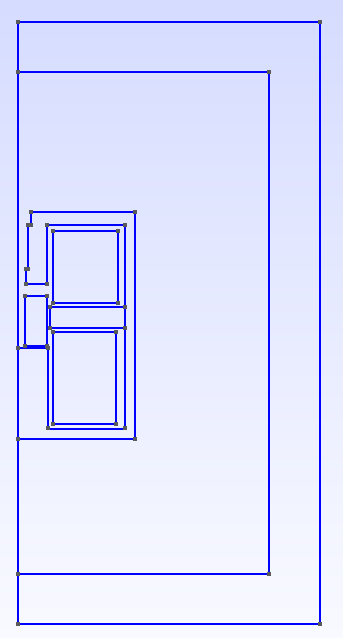
\includegraphics[width=0.35 \linewidth]{figures/model.png}
	\label{fig:model}
	}
	\hspace{0.16 \linewidth}
	\subfigure[Qt实现填充区域]{
	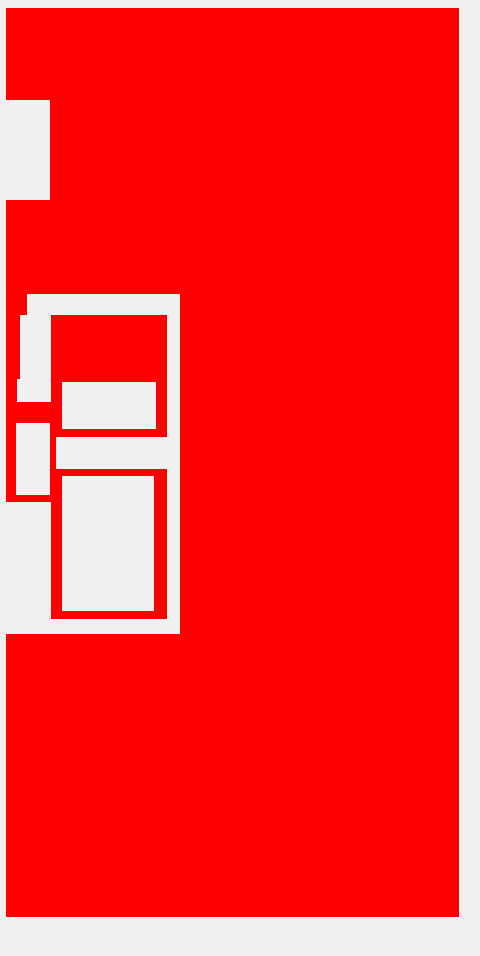
\includegraphics[width=0.33 \linewidth]{figures/path1.png}
	\label{fig:path1}
	}
	\caption{CAD模型以及空气区域的填充效果}
\end{figure}
然后令人比较惊奇的是,这个类还可以检测点是否在路径的内部,虽然并没有搞懂绘制路径的原理,但是莫名的好使,需要进一步研究路径的原理来使用它。

在填充路径时要用到填充规则,这里一共有两个填充规则

path.setFillRule(Qt::OddEvenFill);//奇偶填充规则

如果要判断一个点是否在图形中,可以从该点向图形外引一条水平线,如果该水平线与图形的交点人个数为奇数,那么该点在在图形中。

只填充在图形内的点

path.setFillRule(Qt::WindingFill); //非零弯曲规则

如果要判断一个点是否在图形中,可以从该点向图形外引一条水平线,如果该水平线与图形的边线相交,这个边线是顺时针绘制的,就记为1,是逆时针绘制的就记为-1,然后将所有数值相加,结果不为0,那么该点就在图形中。

QPainterPath判断点在内部的算法:

1.检查path是否为空,点是否在path的边界内;

2.根据path当中的元素进行迭代;

3.针对每一个path,按照上面的方法,做一条水平线,计算交点的个数,最后统计交点的总数,如果是奇偶填充规则的话,偶数就代表不在区域内部,不填充;奇数代表在区域内,填充;如果是windingfill,就判断曲线的逆时针和顺时针的方向,最后求和是不是0。

但是,具体填充的是否不会是这样判断的吧,如果是这样的话,计算量有点大啊。
\subsection{建立face}
可以简单的建立face,保存数据并不困难,难的是怎样把face绘制出来。一般的face的话,采用填充就可以了,但是对于有嵌套的face,填充就不好使了,可以想到的办法就是使用qt当中的path来绘制,它的绘制原理是按照奇偶填充绘制的,能够实现所想要的效果。
\subsection{如何保存tree的展开状态?}
应该是要保存哪些节点需要展开,哪些节点需要折叠。
\subsection{关于单元建模}
主要纠结的地方在于,单元的保存格式跟几何形状的保存格式并不一样,如果单纯的按照一方来保存,是不是过于强耦合?现在的逐步的感觉难度在于建模方面,你要考虑有限元当中的模型,cad的模型,绘图的模型,还有求解的线性代数的模型,每一个都需要有实际的经验来进行设计,不一定你设计的就是最好的,但是一定得是有道理的,主流的方法。
\subsection{如何使用gmsh的链接库?}
如果能够使用gmsh的链接库,那么就可以使用其中的大量的api进行操作,就不比只使用exe操作有用的多。


\subsubsection{插件如何翻译}
目前还是在一个文件里进行翻译,好像没什么能够合并的方法。
\subsection{模型传递的问题}
鉴于传入到求解器当中的参数很多,

\subsection{复杂几何模型问题}
很明显,将过多的精力放在并不擅长或者永远见不到头的CAD上面是不够明智的,只需要满足最基本的需求即可,过多的功能无需实现,也没有必要实现,COMSOL也不见得能够建立多么复杂的模型,退而求其次的方法就是具备几何模型导入和分网导入功能,这样对开发进度是一个很好的解脱。
\subsection{坐标系的种类}
常见的坐标系有:笛卡尔坐标系(也就是直角坐标系),圆柱坐标系,极坐标系。根据对称性来分类,无对称,有对称面,有对称轴。
\subsection{如何设计solver的位置?}
求解器,准确的来说只是一个求解的函数,但是如何进行合理的设计,利用好cpp的类的设计风格?感觉c当中的那种纯函数的风格更加的不错,可以直接调用。其实cpp的类当中不一定需要设计成员变量,可以出现没有成员变量,只有函数的情况,也可以存在只有成员变量,没有函数的情况。但是,其实后一种编译器会自动的添加默认的构造函数和析构函数,同时,也要求你的类成员变量需要有默认的构造函数,否则编译器就无法调用准确的构造函数完成初始化任务。
\subsection{有限元装配原理}
在大多数的有限元求解当中,是需要矩阵装配过程的。也就是将有限元的单元矩阵合成为全局矩阵,然后进行后续的迭代求解。根据矩阵的格式,可以分为全矩阵和稀疏矩阵两种格式。如果是全矩阵的话,装配过程就相对比较简单,只需要将矩阵元素跟全矩阵对应位置的元素相加即可。如果是稀疏矩阵,最后生成的格式是对应的稀疏格式,装配起来就会复杂一些。具体的可以参考文件SpMat\_meat.hpp。

我觉得生成的思路有好几种,一种是直接生成的,将所有非零元素的值和位置进行保存,由于同一个位置可能有多个相加值,然后需要计算出每一个位置的相加后的值,得到位置与非零值的对应数组,最后就是将数组进行压缩,就得到稀疏矩阵的保存格式。

另外一种方法就是,使用死办法先创建一个全矩阵,然后将装配结果保存到这个矩阵当中,全矩阵的好处就是检索比较方便。由于全矩阵很占内存,最后再将所有的0去除,得到非零元素,最后再得到压缩后的稀疏矩阵格式。
\subsection{细节}
最不缺少的是流程图和框图。因为上面等于什么也没说,想要实现的话还得看细节。大家都知道步骤A之后是步骤B,但是问题就是如何过渡过去的事情。接口这事情,没有经验,最开始是写不不好的,还不如先不写,最后需要扩充的时候再写。
\subsection{捕捉实体}
为了实现实体形状的选择,就要依靠鼠标指针的位置来判断是否在形状的范围内。看上去似乎很不错,但是有一个问题,有些形状是最基本的,不可以分割的,而有一些形状就是由其他形状拼接过来的,比如矩形就是四条直线拼成的。那为什么不让矩形不可拆分呢?
\subsection{filelistchanged}
采用信号槽的方法来动态的更新列表。主要是要对那几个顶部的node进行操作。

Project::handleSubTreeChanged -> ProjectTree::emitSubtreeChanged -> ProjectTree::subtreeChanged -> FlatModel::updateSubtree -> FlatModel::addOrRebuildProjectModel

对于树的更新,有两个方面,一个是刚开始的时候创建了一个project,这个时候需要添加一个项目添加的处理,就要build一下project,这个是一个信号,就是添加项目,然后我自己修改tree的话,就不再是添加了,而是tree的改变了。tree的改变也是一个信号,也需要调用rebuild的操作,那是如何保证不改变原来的部分呢?就是每一个项目的根节点,它对应的都是一个项目,在改变tree的时候,先要找到project对应的根节点,然后把它的所有的children给清空,然后在这之前你需要更新一下projectnode,然后就可以把projectnode添加为到treeitem。所以,问题就在于,如果更新了node,之后,就需要重新生成projectnode。

现在终于看懂了,主要有两条线,一条是node,另外一条是treeitem。其实之前主要忧虑的地方在于移动之后,node还在不在了,移动之后,指针的指向还是正确的,只不过不再属于原来的变量了。由于node的保存是树状的,最后都会跑到顶部节点下面,还是只能能够检索到子节点,还是能够正常访问的,内存并没有被释放,数据也没有丢失。这是project的node列表。为了能够在控件上显示树列表,就要把node转化为model当中的treeitem数据,这个也是按照树结构保存的,所以只要调用递归函数进行生成就可以了。model就可以自动的根据调用函数来读取所有的items。然后其他的编辑访问操作,都是最后读取到对应的node。为了添加或者删除node,先是要通过tree获得当前选中的节点,然后对该节点进行操作就可以了,然后发射树改变的信号,就能实现tree的改变。

我成功地按照这种方法添加了子节点,但是,需要弹出对话框来设置材料,要是能够获得dialog的执行结果就好了。这样就能进行判断。每一个对话框会返回accept结果或者reject结果。

我可以寻找各个标志所在的node,
\subsection{对话框的创建}
在软件的运行过程当中,肯定会有很多的对话框出现,应当以ui的方式建立窗体还是以代码的方式建立窗体?还有,如何批量的建立窗体。

从功能上讲,ui和代码设计都能达到相同的效果,当然,代码的能力可能会更强大一些。
\subsection{创建tree的右键菜单}
1.先在actionmanager当中创建一个菜单的ActionContainer*,这个manager已经在主窗口当中进行了初始化了;

2.然后在菜单当中创建所需要的group,每一个group都代表了一类功能,group是一个特定字符串代表的值,不同的container可以含有相同的字符串,就像每栋楼都有101房间一样,默认的,为了防止将action加入到一个空的container,container自带三个group,会将没有id的action添加到这三个的其中一个;

3.接下来就是给各个group当中添加actions,在添加第一个action之前,需要添加一个分隔符,然后就是不断的添加action到对应的group了。同一个action可以添加到不同的group当中。小技巧就是,在h文件当中定义一些group的常量名称。

4.在treeview的showContextMenu函数当中,根据不同的节点类型,调用显示不同的菜单。
\subsection{如何统计代码的总行数?}
采用正则表达式进行匹配搜索,但是有误差。
\begin{lstlisting}
	b*[^:b#/]+.*
\end{lstlisting}
\subsection{armadillo中的稀疏矩阵装配过程}

\subsection{绘制方形的时候,直线不黑,严重虚化}
感觉是在坐标强制转换的时候出了错误,有的时候会差一个像素点,导致参考点绘制的时候不在中心上。而且有的时候,一条黑色的直线会画成两条,一条灰色的,一条黑色的。有的时候就没有。如图\ref{fig:linemohu}所示。
\begin{figure}
	\centering
	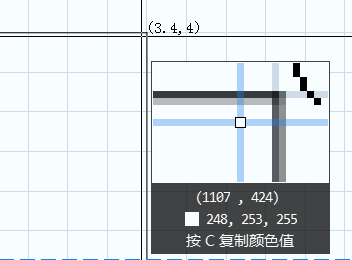
\includegraphics[width=0.7\linewidth]{figures/linemohu}
	\caption{绘制的直线不黑,模糊}
	\label{fig:linemohu}
\end{figure}
发现这并不是偶然出现的,而是确实哪里有问题。我们来查找一下原因。绘直线最基本的就是两个点,如果两个点的坐标算错了,那么画出来的图有可能因为变歪而显得模糊,因为水平和竖直线肯定总比斜线要清晰。但是经过排查,其实坐标没什么问题,虽然它使用了float类型的point,但是我觉得这不是问题所在。那问题就可能出现在绘制的过程当中。接下来不断地进行跳转到drawline函数的实现,发现在绘图之前需要判断是否要抗锯齿化,只有设置了抗锯齿化之后才会变得清晰。所以,问题就变成了确认一下在绘制直线的时候是不是抗锯齿化的,如果不是,那么这就是问题所在。发现drawline并没有被显式地设置抗锯齿化。

需要注意的是,实际的坐标值转化为像素点的时候,它不是一个整数,肯定会有小数位,然后你绘制的时候,可能就是以像素点为标准绘制的,严格意义上讲,是不准的。反过来,你捕捉点的时候,你捕捉的是像素点,然后你将像素点转化为坐标点,这个值也是不能跟实际坐标点完全对应的,肯定会有误差。需要知道qline和qlinef的区别。从文档中来看,这样做只是为了扩大坐标点的存储范围。
\subsection{treemodel是如何建立索引的?}
父索引,也就是root索引这个肯定是有的,有了这个,就可以递归的生成其它的索引了。所以,下一步就是在project当中定义model,然后在treemodel当中添加对project的处理,这样就可以了。可以先在内存当中测试,等到测试没有问题了,再添加对文件的读写。

\subsection{是如何达到效果的?}
通过反复印证。
\subsection{属性页如何实现}
需要点击树控件上的每一行,切换页面,还是qstacklayout?
\subsection{Node的设计}
主要针对于树控件当中的Node的设计。树控件是重要的交互界面。先找到问题,然后尝试在各种情景下复现问题,分析问题产生的原因,定位使问题产生的环节,最后尝试修复该环节。

没有子节点的Node可以有两种,一种是在定义实现当中没有子Node,未来也无法扩展该功能,另一种就是有子Node,但是在接口上没有实现,未来根据需要可以进一步地开发。为了避免Nodes随意的插入,是不是可以加入排序功能,将相同的Node排序到统一的节点下,但是,在某些情景下,Node之间的相互顺序是很重要的。

为了避免Node插错位置,我觉得需要在插入的时候进行类型判断,如果类型不对,就不让插入。或者,每一个node设定一个级别属性,级别低的不能插入到级别高的node下。应该是tree的列数吧,根部节点只能插入到第一列,二级节点插入到第二列。

同时,还要考虑数据存储的问题。

基类的Node。感觉这里的node之间没有什么特别明显的继承关系,都挺孤立的。

\subsection{材料库}
预先准备好材料库文件,打开对话框之前,读入文件并且显示。不同的物理问题对应的材料库应该不同。因为他们所关注的属性不一样。所以,这就给建模带来了一个问题。每一种材料的属性都要建的非常全面。
\subsection{生成树的算法}
如果存在project文件,准备文件;

分析文件;

写node。

这是针对硬盘上的数据,如果是内存当中的数据,本身不会采用文件的这种格式,而是具体的数据。总结起来,有三个数据,一个是硬盘上的,一个是节点node,一个是真实的变量。这三个应该如何权衡之间的关系?我认为大体的思路是没有错的,只不过可能比他们更加缺少对实现细节的考虑或者对功能的设计。按道理讲,三者的数据应该是同步的,一个对数据进行了修改,其余两个都要进行改变。关键在于辨别那个数据才是最新的。project最初打开,最终保存的时候,会涉及到硬盘文件存储,在整个其他的操作过程当中,可能都是在内存当中存储的。project应该和node共享变量指针。

“两年前我还在折腾Linux Kernel的时候, 正碰上他们组发表了一篇修改Linux内核的锁实现, 以在众核(单机超过32核)情况下提升应用性能的文章. 文章效果非常好, 使用的几个workload都达到了近乎线性的加速比. 我在学术讨论会上报告这篇文章的时候, 大老板听闻这篇文章只不过编写了1600+行代码, 大手一挥让我们大干快上, 也搞个类似的出来. 可是改内核这种事情, 别说修改1600行, 就是改一行代码, 想要知道在哪里修改能够取得预期的效果, 对普通的博士生来说其背后的工作量都是难以估算的. ”
\subsection{vs code and $\LaTeX$}
已经看不惯了texstudio那样丑陋的界面了,心动之下打算尝试一下vs code。首先,vs code的启动速度在新电脑上没有那么慢,而且界面风格比较喜欢,网上也有很多设置latex环境的方法,非常简单。只需要安装latex workshop的插件就可以了。还可以设置pdf的正反向搜索跳转。需要注意的是,如果使用的是sumatrapdf软件,并且是在vscode的左侧树当中打开的这个软件,那么,似乎是因为这个是属于vscode的一个进程,所以,反向跳转可能会不好使。需要单独地在外部打开软件进行跳转即可。真的是非常喜欢x1c打字的键盘。清脆。尤其是高清的屏幕看起来非常有质感。但是还不知道怎么设置正向搜索,哈哈。
\subsection{模块之间开发不同步的问题}


\subsection{有一个问题}
在开发的过程当中,发现不管是要实现的函数,要规划的任务,都实在太多了,一不小心就不知道开发到什么地步了,什么功能有没有实现,实现到什么程度了,有没有被测试,有没有bug,好不好使。应当有那样的一个任务板,设定好要实现的计划和任务,明确规定功能的详细内容以及预计完成的日期。
\subsection{插件放哪里?}
插件的声明,应该放在mainwindow当中吗?从插件的功能来看,这就不属于主窗口的东西,而是独立于它的一部分,但是由于主窗口留出了访问其内部资源的接口,所以,也不必在mainwindow中实现。

但是,这是人家插件系统当中的版本。人家是通过一个插件管理器来载入了所有的插件,进而能够访问所有的资源和功能。反正怎样写都可以实现。如果是单独开发的话,写到main当中,这样集成度更高一些,因为这本来就是自己写的,而不是第三方,所以为什么不能放进去?可以的。但是,一定要注意初始化的顺序,有些插件是依赖于别的插件的,有先后顺序之分的,不然资源还没有被创建,后面的都JJ了。
\subsection{qDebug重定位}
我有一个大胆的想法,在调试的过程当中,总是要去看qtcreator的输出信息,窗口要切换来去非常的繁琐,要是直接能够把信息定位到我的log窗口,那么就不需要切换窗口了。之所以想定位debug,是因为不想改太多的代码。

仔细地查了一下资料,实现的原理很简单,就是重新实现一个qdebug,也就是定义一个新的宏命令吧。
\subsection{绘图的交互}
在绘图的时候,是设置为必须先绘制所有的点,然后再连接得到线段,最后再生成面。还是,可以随意的绘制。

第一种的好处就是,整个图形都是由最底层的点的坐标组成的,只要修改点的坐标,整个图形就可以相应地进行更新,而另外一种,就必须对每一个图形进行修改,因为它的坐标都是内部的,与其他的没有什么联系。
\subsection{生成面的算法}
刚开始比较好奇计算机是怎样实现不规则形状多边形的填充的,就搜索了一下奇偶填充算法,真的找到了很多资料,有很多的算法。看着看着就看到了一个主题,平面内封闭区间的识别,这个问题应该与生成面的算法类似吧?看到有人提出用计算图形学当中的一个漫水填充算法,这个名字真的好形象,在区域内找一个点,然后就开始递归式的开始填充,如果没有碰到边界,就不断地向前搜索,最后所有的区域都被填充了。但是效率实在太低了,每个点都要进行判断。

但是,还是不如直接设置方便啊。数据量小的话,还是手动设置吧!
\subsection{treemodel}
qmodelindex这个变量它所指向的东西可能会变,因为它的含义是某行某列,而模型当中可能会插入一些数据,导致它的行列数已经发生了改变。但是index当中不是保存了数据的真实指针了吗?
\subsection{图形选择}
选择的实体,是要单独的保存出来呢,还是要标记为“选中”状态就可以了?按道理讲,没必要那样做。选中状态的效果,是采用了不同的笔刷来实现的,只要跟正常画的不一样,就会给人以选中的状态,因为在单击鼠标的那一刻,图形颜色改变了,有反馈说明被选中了,因为只有选中了才会有改变啊。cad并没有在每一个形状的draw函数当中单独的进行选中的判断,而是放到了graphicview当中集中处理。这样的好处就是节省代码量。

绘制图形前需要判断:
\begin{enumerate}
	\item 是否存在;
	\item 是否可见;
	\item 是否在显示区域内;
	\item 设置笔刷;
	\item 是否被选中;
\end{enumerate}
\subsection{调试}
大型软件怎么调试?光是编译有时候可能都得十几分钟,有的甚至有几小时,几天的,这种情况还整个跑起来调试不太现实吧,应该都是单个模块调试吧。
\subsection{更新}
以谁为更新依据原理应该是谁先获得焦点。

\subsection{menu}
之前在顾虑ribbon的page上的每一个group都是一个控件,没办法插入菜单。但是,似乎理解不够,抽象不够彻底。group上面的动作,可以通过添加action来实现,menu本质上也是一种widget,所以group也是可以插入menu的。
\subsection{tree与node}
还是搞不清楚之间的关系。我觉得大型软件编程有这么几个问题:第一,要有非常明确的需求,不论是怎样的幻想,设计,最后都要落实到具体的细节上,而不是简单的,我就是想要实现一个类似什么的功能,同时,也要避免后期的无端的需求变化;第二,不只是只有我有这种想法,我曾经以为计算机科学课上学过的“面向对象”是很简单的东西。我的意思是,创建一些类来模拟现实世界能有多难啊?其实,那还真是挺难的。需要学习如何合理地建模,花更多的时间来学习面向对象和设计模式。优秀的建模技术对于每一个开发团队都是非常有价值的。第三,软件吸引客户的地方不在于你的核心求解算法有多牛逼,而在于真正地满足需求。

explore是怎样新建项目,打开项目的?具体做了啥?项目内容是怎样更新到tree控件上的?反过来,tree控件上的东西是怎样更新到项目文件的。中间的接口在哪儿?tree上的节点应该全部更新还是只更新发生变化的?如何判断哪些发生了变化?新建项目的时候,应该会出现一个wizard,如果没有的话,就是建立一个默认的项目,然后将项目添加到session当中,根据提前设置好的信号,会同步触发treemodel的更新处理。每一个project都能够根据自己的数据build一个tree模型返回。新建项目的过程可能是这样的,先创建一个项目文件在硬盘上,然后再调用打开项目的函数。

应当有两个buildtree的过程,一个是根据project当中的数据生成对应的节点,一个是将节点转化为treeitem。什么时候将project当中的数据生成节点?构造的时候会。其他时候?应该是建立一个观察器,观察项目的变化,
\subsection{面向对象的类的设计}
\subsection{上下文}
上下文到底意味着什么?

\subsection{项目文件保存需要注意什么}
随时都会对项目树进行操作,就会产生新的数据,需要立即保存吗?保存的话可能是在文件中插入,是重新保存一次吗?
\subsection{signals 和 slots}
这两个东西我都理解是什么 ,但是有一个问题,什么时候需要自定义signals?
\subsection{如何测试?}
有数不清的函数和类文件,大多数有很大的依赖性,如何脱离项目完成单独的测试?

\subsection{单元测试}
单元测试好像不是我所认为的测试。
\subsection{材料}
如何定义材料类,也是一个非常值得研究的事情。因为,材料实在是太复杂了。有着数不清的属性。在某些研究当中,只有某几个属性有利用价值,其余的没有使用价值。如果定义一个包含所有属性的类,必然会浪费很多的空间。那么就应该具有添加自定义属性的功能,根据需要生成某些特征。
\subsection{qtcreator的模式}
需求分析,定制功能,任务拆解,技术支持,功能实现。设计的思维,理念,技巧,套路,模版。

以主窗口为核心,对外提供操作的接口。接口的当中提供的控件不会无故添加在主窗口当中,需要提前在这个类当中提前声明控件的指针,并提供接口。
\subsection{函数的实现}
类当中的成员函数,不一定要在对应的cpp文件当中全部实现,可以在h文件当中实现,也可以分散在好几个文件当中实现,有时候采用这种方式可能是为了调用该文件当中的某一个函数,或者要被调用。
\subsection{有限元求解的必要因素}
为了完整的求解一个有限元问题,需要那些因素?注意,是所有的,而不是一些不可缺少的,有的问题需要而有些问题不需要的。
\subsection{有限元类的设计}
所有的求解变量都应该存储在project类当中,包括几何模型、材料、物理属性、分网等等数据,因为求解当中是以project为核心的,不能将数据放置到别的地方,这样就容易被其他的项目修改。同样的,一系列的求解操作都应该放在project当中进行实现。

那么有一个问题,是projecttreewidget包含project还是project包含它?应该是比project更高的一级拥有这个东西。
\subsection{如何规定当前求解问题的类型?}
如果不设计更加具体的project子类,通过什么方法来辨别求解问题的类型,所需要的物理公式?真的能够多物理场吗?
\subsection{信号槽}
只有真实的对象之间才能产生信号槽。克服屏幕分辨率低,显示像素差的方法就是放大字号。
\subsection{菜单}
如何在系统栏添加菜单?这个操作并不是在主函数当中一次完成的(指的是插件风格的写法),每一个插件都有跟自身相关的操作菜单,所以这部分菜单的生成可以放在对应模块的初始化部分执行,这样更加具有合理性。随用随加,用完就删。但是这样的写法还没有针对ribbon风格进行测试,毕竟ribbon的api似乎没有menu那样的丰富,不知道最后的显示效果会是什么样。不知道ribbon和menu之间有没有一些转换的函数。但是ribbon比menu的高级的地方在于,ribbon当中可以放置更加复杂的widget。另外一个ribbon需要解决的就是,能不能在任意一个group之前插入,如果可以的话,就可以对照着menu进行修改了,但是还是觉得效果可能没有menu那样的优雅。
\subsection{menu与group的区别}
在一个menu当中,插入一个menu,效果就是插入了一个子菜单,但是如果插入了一个group,就是插入了一组动作,菜单列表是在一级显示的。对于菜单,可以不断地嵌套式地插入,但是,ribbonbar的widget控件就不能这样干了。
\subsection{运行当中的无效菜单如何设置?}
通常,软件当中,根据运行环境的判断,某些菜单在这个情景下可能会失效,这个效果如何才能实现。实现的原理就是添加一个信号槽,信号就是菜单将要显示,连接上更新菜单的动作即可。
\subsection{SessionManager是干嘛的}
这个貌似是一个项目管理与当前运行之间的一个接口。
\subsection{磁材料建模}
线性、非线性材料;
\subsection{导航控件}
没有写代码之前,没有研究别人的代码之前,并没有认识到自己想法的单纯和简单。也就是没有什么经验。对功能的认识不够清楚,研究地不够明澈。可以说,理解的非常的狭隘,不利于代码实现。例如,最开始对项目的认识,以为就是一个对xml文件进行读写的类,可是仔细的研究别人的写法,发现并不是这样的,或者说并不是全部。project类并不是项目插件的核心,只是一个小的模块,你不可能只是只打开一个项目,所以你要管理项目,项目还会有很多添加删除的动作。项目不光有数据,还要有控件,而这个树控件,肯定要包含一些跟项目有关的东西,所以它不能是标准的树控件,必须对他进行自定义,添加自己的数据模型。然后把这些都封装进project的模型当中,然后再把project放进项目管理器当中进行管理。项目这块儿是绝对的核心,其他的什么编辑器啊,别的都是被调用的,用来显示项目当中的数据的。最好的设计方法就是要把足够独立的模型给建立成一个类,利用类之间的包含关系,再建立更加复杂的对象模型。导航控件不只是只有树,还有其他的按钮之类的,所以应该单独地建立为新的控件。
\subsection{dockwidget}
如果在窗口当中添加了dockwidget,好像是自动带分割器的,如果就是普通的,那么就得自己加吧。
\subsection{ui当中的文字怎样翻译?}



\subsection{项目树}
分析分析项目树的设计。

\subsection{zoom in and zoom out}
放大和缩小最常用的地方就是鼠标滚轮,以一个点为中心进行缩放。缩放的时候,先调整整个区域的边界大小(显示大小),然后再将缩放点移动到原来的位置,这样就是以该点为中心进行缩放的了。

以某点为中心进行缩放,意思是该点与另一点之间的距离按比例缩放,而中心点的位置不发生改变。

缩放有方向的问题,如果坐标轴不是等比例的话,会有水平和竖直两个方向上的缩放,如果是等比例的,那就对任意一个方向进行缩放,都会达到相同的效果。

那如果使用按钮来操作缩放,中心点应该怎样算?坐标轴的中心还是鼠标指针的位置?

是什么问题?在现版本的操作当中,由于绘图都是在坐标轴内部的,所以,只要对坐标轴进行rescale就可以了。
\subsection{坐标轴的resize问题}
cad控件的显示区域大小是受到窗口影响的,在调整窗口大小之后,应该如何合理地显示图形?
\subsection{project文件}
项目文件应该如何正确的读取和写入,应该如何设计。

project文件的读取过程:

1.调用读取多个project的函数;

2.进入子函数;

3.已打开的project和未打开的变量,打开结果;

4.进入循环读取,循环过程如下:

5.判断文件名是否为空;

6.判断文件是否已打开,则进行一些处理后跳过;

7.打开文件,对文件进行判断,不存在则返回;

8.调用project的构造函数,生成变量,项目的打开是一个对文件的语法分析过程,并保存分析的结果;

project的信息是以node树的方式保存的,然后把它传给treeitem变量,之后就传给了treewidget控件了。初步掌握了一下对node的操作,原版的node写的真的是好绕啊,你要显示一个tree,你要有一个model,一个view,而且还要有你保存数据的模型,model当中不是用来保存你的数据的,而是根据你提供的数据,编写一个给qt的计算接口,这样它就知道如何根据你的数据,得到哪行哪列的具体数据了。

具体的数据是保存在treeitem当中,而WrapperNode类它不是Node类型的,而是treeitem类型的,里面相比多了node变量。treeitem类的主要作用是描述了数据的树状存储关系。node变量如果是container类型的话,它也是嵌套的树结构。所以,treeitem的能力并不只是表示树中的一个节点,那样的话跟node有什么区别,它应该还可以表达tree当中的一段。之后,通过研究源代码,发现确实生成了treeitem的树变量,首先传入projectnode变量,里面包含了所需要的东西,然后再进行递归处理,生成tree,最后就可以在控件当中显示了。


9.做一些其他的后续处理。
\subsection{读完project怎样更新treewidget?}
什么是projects?里面应当保存什么东西?projects是一个完整的个体,从存储角度看,projects是硬盘上的一个文件,保存你所需要的所有的信息,是最终的实体。因此,projects类就是对该文件的一些操作接口,将硬盘上的文件信息,保存为内存中的模型数据。需要进一步考虑的问题是,projects是否单一,是否具有多态属性,是否需要建立子类。其实这个只是一个写法的问题,最后都能实现功能。还有一个问题,就是最后效果只是单一的projects,但是在代码的实现上,也可以利用多态虚函数进行实现。
\subsection{如何管理projects?}

\subsection{类的工作流程图}
所有类之间的工作流程图是怎样的?

\subsection{状态的改变}
我们通常会采用emit signal的方式来通知别的对象执行某些操作。但是有一些问题,比如,发射信号的变量是动态创建的,怎么能保证能通知到呢?这个时候可能需要一个静态的管理器,通过发射信号来再次靠管理器发射一个信号,只需要将执行的一方和管理器的信号连接起来就可以了。
\subsection{为什么会有一个treewidget的list?}
按照一般的想法,不是应该只有一个projects的树控件吗?那么为什么放了一个list,意味着有多个?那多余的是干嘛的?
\section{编译错误}
\subsection{error LNK2019: unresolved external symbol compress referenced in function}
如果使用Qtcreator出现了这个问题,恰好编译器是vs的话,有可能是一下原因:确定一下在pro文件当中,头文件列表和源文件列表中被调用函数的源文件是不是出现在了调用文件的后面,如果是的话,将它移动到前面去。
\subsection{VS不同版本编译报错}
出现“无法找到文件MSVCP120D.DLL”的问题,问题在于某些使用的dll文件是vs2013生成的,而现在使用的vs版本不是2013,解决方法就是将这些dll在新的vs下重新编译。
\subsubsection{warning: comparing floating point with == or != is unsafe}
\subsection{warning: C4819: The file contains a character that cannot}
你的源码是不带BOM的UTF8格式,但是MSVC不知道你用的UTF8。由于你在简体中文Windows系统下,它就认为你用的是GB18030(也叫GB2312,GBK,CP936)。

当你一个汉字时,占3个字节,用GB18030是无法解析的(1个半汉字)。当你2个汉字时,占6个字节,用GB18030碰巧可以解释成3个汉字。

如果不指定的话默认是 utf-8。所以我们用 gcc 时很少关注这个问题。

Viual Stdio 中就麻烦多了。这里先说 Visual stdio 2015,这个是我现在用的编译环境。VS2015 中如果源代码是 utf-8的,执行字符集默认是本地 Locale 字符集,对于简体中文的 windows 系统来说,这个 本地Locale字符集是 gb18030。所以直接显示汉字会全是乱码。解决这个乱码有三个办法,第一个办法是编译时加入命令行参数,在 Qt 的 pro 文件中可以这样:

msvc:QMAKE\_CXXFLAGS += -execution-charset:utf-8
1
第二个办法是在源文件中加入:

\#pragma execution\_character\_set("utf-8")
\subsection{MSVC中文注释导致的编译错误}
遇到这个问题是将代码在虚拟机下面进行编译的时候出现的。在另外一台电脑上编译运行没有任何问题,但是在这台电脑上运行就好几百个问题,刚开始也是丈二和尚,后来慢慢领悟到应该又是中文编码的问题导致没有正确的解析源代码。

为什么会出现编码错误呢?主要是中文的存在。编码主要存在在两个地方:一个是IDE需要知道文件的编码来正确地进行源代码的显示;第二个就是编译器需要知道文件的编码来正确地对代码进行编译。我们所遇到的错误就是第二个导致的。这个问题的根源在于MSVC编译器对UTF-8编码支持的不是很好。简单来说,就是在Windows下,微软创建的UTF-8文件都自带BOM,而UNIX系的UTF-8文件则不带。MSVC编译器则是通过判断文件有没有BOM来确定是不是要采用UTF-8编码,所以Unix下的UTF-8编码文件拷贝到Windows下使用MSVC进行编译就会不通过。没有BOM,编译器就会采用操作系统的本地语言编码进行解释,中文应该是GB2321。这就很愚蠢了。

解决办法主要有以下几种:
\begin{enumerate}
	\item 将所有的UTF-8文件都加上BOM。这个方法虽然可行,但是不适合跨平台,而且BOM有可能在别的地方打开之后被删掉。还有那么多文件都要批量添加BOM。
	\item 所有文件的编码都改为UTF-8,注释一律用英文。经测试,这个方法可行,没有报错。但是不支持中文注释也太傻逼了吧,都什么年代了。
	\item 所有的文件编码依然采用UTF-8,这样可以跨平台,但是想办法让编译器忽略掉中文注释。注释本来就是被编译器忽略的一部分,但是因为解码错误,编译器只能识别出注释的开始部分,也就是"//"。但是后面的中文如果识别不出来的话,就会连带注释后面的英文代码也变成了注释,直到解析出了换行。所以解决办法就是让编译器识别出注释的结束,想来想去,只有多行注释这种方法了,也就是“/**nnnn**/”。经实测,这种方法可行,但是就是得两个星号。
\end{enumerate}

详细的解释可以参考:\url{https://blog.csdn.net/imxiangzi/article/details/50781459}、 \url{https://www.cnblogs.com/Esfog/p/MSVC_UTF8_CHARSET_HANDLE.html}、 \url{https://www.cnblogs.com/cheungxiongwei/p/8003867.html}、 \url{https://blog.csdn.net/liyuanbhu/article/details/72596952}。
\subsection{error: LNK2019: unresolved external symbol referenced in function}

明明没有什么问题的项目编译之后却报这个错误,开始的时候确实令人匪夷所思。在另外一台电脑上编译运行也没有什么问题。解决办法就是将build目录删除,然后重新编译运行,就没有这个错误了。
\subsection{vs2017 char *}
在新版本的vs2017当中,向函数参数传递常量字符串的时候,会无法转换的错误。这个错误产生的原因似乎是由于在C++11的标准中,不能直接将常量赋值给指针变量,解决办法就是在常量字符串前面加上指针的强制转化符。
\subsubsection{error: Failed to resolve include "debug/moc\_predefs.h" for moc file QtnRibbonSliderPane.h}
\subsection{error: C2039: 'unique\_ptr' : is not a member of 'std'}
vs2013 好像不支持这个。完犊子。用vs2017写的。
\begin{lstlisting}
	#include <memory>
\end{lstlisting}

加上这句即可。
\subsection{signal没有响应}
qt当中,已经设置了信号并且进行了连接,为什么没有响应?没有执行任何函数,在信号发出之后。肯定是哪里跳出了。。。
\subsection{如何编译superLU的dll?}
之前使用superLu的时候,都是编译的静态库,但是如何采用动态库呢?我在vs当中把生成目标改为dll不成功,报错。后来我想了一下,lib文件就是一个obj文件打包的过程,但是dll之前在使用的时候,确实需要export操作的,只有这些export的函数或者变量才能被外部调用。
\section{其他}
\subsection{Texstudio与sumatrapdf反向搜索关联}

sumatrapdf是一款免费小巧的PDF阅读器,双击PDF的某一个区域,可以打开关联的tex文件的相应位置。对于winedit,"D:/My Program Files/CTEX/WinEdt/WinEdt.exe" "[Open(|\%f|);SelPar(\%l,8)]"
对于TeXstudio"D:/My Program Files/TeXstudio/texstudio.exe"  "\%f" -line \%l

\section{已知Bug}

\subsection{UI}

\begin{enumerate}
	\item QtFlex 的控件从左侧停靠到再次显示时,控件跑到了右侧停靠去了。貌似整个的停靠恢复是错误恢复不到原来的状态。另外,停靠显示预览时,也是非常的模糊。具体观察,就是底部或者顶部区域是透明的。
	\item QtFlex 中间的控件变为float状态后,剩余的控件不能立即占满全部空间。
	\item 当处于中心的控件变为float时,指示器应该指示只能放在中心区域。
	
	\item qribbon如果没有从setting读取到一个theme的话,会报错。
	
	\item qribbon的弹出菜单位置有点高,遮挡了按钮上的文字。
	
	\item 在win10下,qribbon最小化,再最大化之后,当前的page会消失。
	
	\item QWidget::mapTo "parent must be in parent hierarchy"
	
	\item qtflex 集成到qribbon窗口中,不能设置标题,会报内存访问的错误。
	
	\item 绘制坐标轴的时候,由于需要设定坐标轴等比例。需要对xy轴进行同时设置。但是问题在于有的时候,新生成的tickerlabel文字宽度发生来改变,导致坐标轴的显示区域发生了变化,但是此时没有及时的更新range和tickerstep,导致坐标轴又不成比例了。而且这个可能会导致递归的问题,如果不断的变化range,文本宽度不断变化,就死循环了。因为是先有的文本,然后计算的rect区域。
	
	\item 在坐标轴区域,鼠标指针莫名其妙变成了调整间距的光标。
	
	\item x坐标在滚轮作用下只能左右滑动,而不能放大缩小。bug分析:由于只设置了x的比例是y的相等比例,所以y轴的刻度才是决定其他坐标轴的关键,其他坐标轴都是被动的。x轴响应滚轮事件之后,虽然计算得到了一个新的range,但是马上又调用replot事件,导致又根据y轴的刻度重新又得到了一个新的x的range,其实还跟原来一样,导致滚轮事件无效。但是滚轮事件使得坐标轴的中心发生了变化,所以x轴的range虽然没有变化,但是发生了左右偏移,所以才有了这个bug。要么就是把单个轴的滚轮事件关掉。
	
	\item 为了使得坐标轴有一个比较好的显示效果,xy轴上的显示刻度数需要足够多,又不能太多,但是默认的刻度值不能适应窗口大小的变化。
	
	\item 所有的实体在绘制的时候都会被绘制两次,因为container类型也是一种实体类型,而实体类型在创建的时候都会被设置一个layer,也就是加入到layer的实体列表当中,而container本身保存的就是一个列表,所以这个列表被保存了两次。一个勉强的解决办法就是不实现entitycontainer的draw函数,那么即使被调用,也不会画出来了。
	
\hspace*{2em}最后的解决办法是,子类在调用父类的构造函数的时候,设置父绘图对象为空,这样,就不会调用setlayer函数,但是还需要在子类的构造函数中完成初始化操作。需要注意的是,此时所有的实体都不是默认再创建的时候被添加到层当中,所以需要手动添加。
	
	\item 在绘制的过程中,如何实现拖拽。比如当前的action是画圆,但是想要拖拽一下调整位置,坐标轴本身是支持拖拽的,但是可能有冲突。可以考虑再添加一个拖拽的判断,如果是拖拽,则新建一个平移的函数。或者也可以长按滚轮键来实现拖拽。要么还可以在每一个图形绘制结束后就结束action,而不是连续模式。
\end{enumerate}	
\chapter{开发进度}
\chapter{版本历史}

\section{0.0.0.1}
\subsection{几何建模}
\begin{itemize}   
    \item 绘制点、线、矩形、圆等;
\end{itemize}
\subsection{分网}
\begin{itemize}   
    \item 三角形分网;
    \item 分网大小控制;
    \item 分网数据导出、导入;
\end{itemize}
\subsection{材料}
\begin{itemize}   
    \item 新建自定义(非)线性电磁材料;
    \item 软件自带部分常见材料;
\end{itemize}
\subsection{求解}
\begin{itemize}   
    \item 二维、二维轴对称静磁场求解;
    \item 磁场分布图形显示;
    \item 数据点提取;
\end{itemize}
\end{appendix}

\end{document}
